% Options for packages loaded elsewhere
\PassOptionsToPackage{unicode}{hyperref}
\PassOptionsToPackage{hyphens}{url}
%
\documentclass[
]{book}
\usepackage{lmodern}
\usepackage{amssymb,amsmath}
\usepackage{ifxetex,ifluatex}
\ifnum 0\ifxetex 1\fi\ifluatex 1\fi=0 % if pdftex
  \usepackage[T1]{fontenc}
  \usepackage[utf8]{inputenc}
  \usepackage{textcomp} % provide euro and other symbols
\else % if luatex or xetex
  \usepackage{unicode-math}
  \defaultfontfeatures{Scale=MatchLowercase}
  \defaultfontfeatures[\rmfamily]{Ligatures=TeX,Scale=1}
\fi
% Use upquote if available, for straight quotes in verbatim environments
\IfFileExists{upquote.sty}{\usepackage{upquote}}{}
\IfFileExists{microtype.sty}{% use microtype if available
  \usepackage[]{microtype}
  \UseMicrotypeSet[protrusion]{basicmath} % disable protrusion for tt fonts
}{}
\makeatletter
\@ifundefined{KOMAClassName}{% if non-KOMA class
  \IfFileExists{parskip.sty}{%
    \usepackage{parskip}
  }{% else
    \setlength{\parindent}{0pt}
    \setlength{\parskip}{6pt plus 2pt minus 1pt}}
}{% if KOMA class
  \KOMAoptions{parskip=half}}
\makeatother
\usepackage{xcolor}
\IfFileExists{xurl.sty}{\usepackage{xurl}}{} % add URL line breaks if available
\IfFileExists{bookmark.sty}{\usepackage{bookmark}}{\usepackage{hyperref}}
\hypersetup{
  pdftitle={Introduction aux Data Sciences},
  pdfauthor={Christophe Benavent - Université Paris Dauphine},
  hidelinks,
  pdfcreator={LaTeX via pandoc}}
\urlstyle{same} % disable monospaced font for URLs
\usepackage{color}
\usepackage{fancyvrb}
\newcommand{\VerbBar}{|}
\newcommand{\VERB}{\Verb[commandchars=\\\{\}]}
\DefineVerbatimEnvironment{Highlighting}{Verbatim}{commandchars=\\\{\}}
% Add ',fontsize=\small' for more characters per line
\usepackage{framed}
\definecolor{shadecolor}{RGB}{248,248,248}
\newenvironment{Shaded}{\begin{snugshade}}{\end{snugshade}}
\newcommand{\AlertTok}[1]{\textcolor[rgb]{0.94,0.16,0.16}{#1}}
\newcommand{\AnnotationTok}[1]{\textcolor[rgb]{0.56,0.35,0.01}{\textbf{\textit{#1}}}}
\newcommand{\AttributeTok}[1]{\textcolor[rgb]{0.77,0.63,0.00}{#1}}
\newcommand{\BaseNTok}[1]{\textcolor[rgb]{0.00,0.00,0.81}{#1}}
\newcommand{\BuiltInTok}[1]{#1}
\newcommand{\CharTok}[1]{\textcolor[rgb]{0.31,0.60,0.02}{#1}}
\newcommand{\CommentTok}[1]{\textcolor[rgb]{0.56,0.35,0.01}{\textit{#1}}}
\newcommand{\CommentVarTok}[1]{\textcolor[rgb]{0.56,0.35,0.01}{\textbf{\textit{#1}}}}
\newcommand{\ConstantTok}[1]{\textcolor[rgb]{0.00,0.00,0.00}{#1}}
\newcommand{\ControlFlowTok}[1]{\textcolor[rgb]{0.13,0.29,0.53}{\textbf{#1}}}
\newcommand{\DataTypeTok}[1]{\textcolor[rgb]{0.13,0.29,0.53}{#1}}
\newcommand{\DecValTok}[1]{\textcolor[rgb]{0.00,0.00,0.81}{#1}}
\newcommand{\DocumentationTok}[1]{\textcolor[rgb]{0.56,0.35,0.01}{\textbf{\textit{#1}}}}
\newcommand{\ErrorTok}[1]{\textcolor[rgb]{0.64,0.00,0.00}{\textbf{#1}}}
\newcommand{\ExtensionTok}[1]{#1}
\newcommand{\FloatTok}[1]{\textcolor[rgb]{0.00,0.00,0.81}{#1}}
\newcommand{\FunctionTok}[1]{\textcolor[rgb]{0.00,0.00,0.00}{#1}}
\newcommand{\ImportTok}[1]{#1}
\newcommand{\InformationTok}[1]{\textcolor[rgb]{0.56,0.35,0.01}{\textbf{\textit{#1}}}}
\newcommand{\KeywordTok}[1]{\textcolor[rgb]{0.13,0.29,0.53}{\textbf{#1}}}
\newcommand{\NormalTok}[1]{#1}
\newcommand{\OperatorTok}[1]{\textcolor[rgb]{0.81,0.36,0.00}{\textbf{#1}}}
\newcommand{\OtherTok}[1]{\textcolor[rgb]{0.56,0.35,0.01}{#1}}
\newcommand{\PreprocessorTok}[1]{\textcolor[rgb]{0.56,0.35,0.01}{\textit{#1}}}
\newcommand{\RegionMarkerTok}[1]{#1}
\newcommand{\SpecialCharTok}[1]{\textcolor[rgb]{0.00,0.00,0.00}{#1}}
\newcommand{\SpecialStringTok}[1]{\textcolor[rgb]{0.31,0.60,0.02}{#1}}
\newcommand{\StringTok}[1]{\textcolor[rgb]{0.31,0.60,0.02}{#1}}
\newcommand{\VariableTok}[1]{\textcolor[rgb]{0.00,0.00,0.00}{#1}}
\newcommand{\VerbatimStringTok}[1]{\textcolor[rgb]{0.31,0.60,0.02}{#1}}
\newcommand{\WarningTok}[1]{\textcolor[rgb]{0.56,0.35,0.01}{\textbf{\textit{#1}}}}
\usepackage{longtable,booktabs}
% Correct order of tables after \paragraph or \subparagraph
\usepackage{etoolbox}
\makeatletter
\patchcmd\longtable{\par}{\if@noskipsec\mbox{}\fi\par}{}{}
\makeatother
% Allow footnotes in longtable head/foot
\IfFileExists{footnotehyper.sty}{\usepackage{footnotehyper}}{\usepackage{footnote}}
\makesavenoteenv{longtable}
\usepackage{graphicx,grffile}
\makeatletter
\def\maxwidth{\ifdim\Gin@nat@width>\linewidth\linewidth\else\Gin@nat@width\fi}
\def\maxheight{\ifdim\Gin@nat@height>\textheight\textheight\else\Gin@nat@height\fi}
\makeatother
% Scale images if necessary, so that they will not overflow the page
% margins by default, and it is still possible to overwrite the defaults
% using explicit options in \includegraphics[width, height, ...]{}
\setkeys{Gin}{width=\maxwidth,height=\maxheight,keepaspectratio}
% Set default figure placement to htbp
\makeatletter
\def\fps@figure{htbp}
\makeatother
\setlength{\emergencystretch}{3em} % prevent overfull lines
\providecommand{\tightlist}{%
  \setlength{\itemsep}{0pt}\setlength{\parskip}{0pt}}
\setcounter{secnumdepth}{5}
\usepackage{booktabs}
\usepackage{amsthm}
\makeatletter
\def\thm@space@setup{%
  \thm@preskip=8pt plus 2pt minus 4pt
  \thm@postskip=\thm@preskip
}
\makeatother
\usepackage{fontspec}
\usepackage{multirow}
\usepackage{multicol}
\usepackage{colortbl}
\usepackage{hhline}
\usepackage{longtable}
\usepackage{array}
\usepackage{hyperref}
\usepackage[]{natbib}
\bibliographystyle{apalike}

\title{Introduction aux Data Sciences}
\author{Christophe Benavent - Université Paris Dauphine}
\date{2021-09-20}

\begin{document}
\maketitle

{
\setcounter{tocdepth}{1}
\tableofcontents
}
\hypertarget{pruxe9face}{%
\chapter{Préface}\label{pruxe9face}}

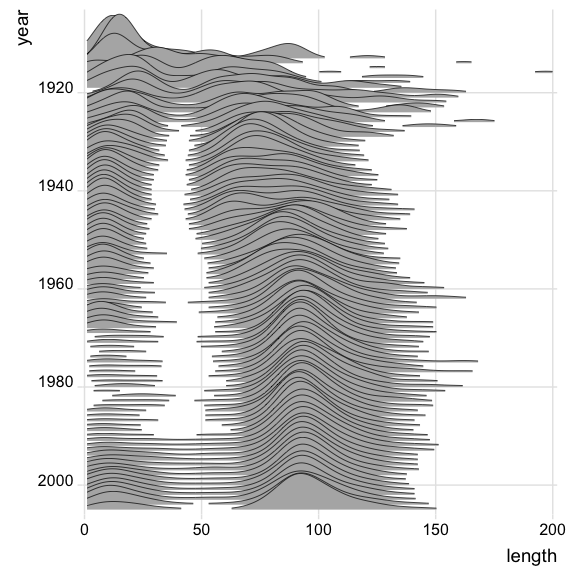
\includegraphics{./Images/ggridge.png}

Ce bookdown reprend les éléments d'un cours de data science avec r. Il a pour but d'être reproductible, c'est pourquoi le choix de ce support et des jeux de données associés. Il sera dynamique, modifié à mesure de nos cours, séminaires et ateliers.

L'illustration représente l'évolution de la longueur des films de la base Imbd et raconte en chiffres une part de l'histoire du cinema. Jusqu'au années la longueur est hétérogène mais au tournant des années 30, la distribution se stabilise, les court-métragessont de l'ordre de 15mn, et voient leurs durée se raccourcir avec les décénnies, le genre menace de disparaitredans les années 80 et reprend du poil de la bête dans les années 2000. Les films longs voient leur longueur s'accroitre et se stabiliser autur de un peu moins de 100 mn, soit une heure et trente minutes. On observera enfin qu'au cours des années 1990 les film de taille intermédiaires réapparaissent.

Dans ce graphique il y a tous les éléments des data sciences modernes : un jeu de donnée riche et systématique, un modèle statistique fondamentale avec la notion de densité de probabilité, une mesure, un critère de comparaison. Les diagrammes ridges sont inspirée de la pochette de l'album \href{https://www.youtube.com/watch?v=7PtvIr2oiaE}{Unknown Pleasures de Joy division} sorti en pleine New Wave , en 1979. Un article de Vice en rappele l'\href{https://i-d.vice.com/fr/article/pabjam/pourquoi-cette-pochette-dalbum-de-joy-division-a-inspire-le-monde-entier}{origine et le destin de ce graphisme}

\hypertarget{plan-et-outils-du-manuel}{%
\chapter{Plan et outils du manuel}\label{plan-et-outils-du-manuel}}

\begin{itemize}
\tightlist
\item
  1 - L'environnement r et python
\item
  2 - Installation et prise en main
\item
  3 - Usage de ggplot - uni et bivarié
\item
  4 - Usage de ggplot - multivarié
\item
  4 - Tables
\item
  5 - AFC
\item
  6 - Clustering
\item
  7 - Analyse de variance et régression linéraire
\item
  8 - Modèles factoriels
\item
  9 - Modèles d'équations structurelles
\item
  10 - Modèles linéaire généralisé
\item
  11 - Modèles à décomposition d'erreur
\item
  12 - Times series
\item
  13 - Analyse geospatiale
\end{itemize}

\hypertarget{les-jeux-de-donnuxe9es}{%
\section{Les jeux de données}\label{les-jeux-de-donnuxe9es}}

Au cours du développement, plusieurs cas pratiques - souvent réduit en volume pour rester exemplaires, seront employés. Les donées seront partagées.

En voici la présentation systématique.

disponibles dans le \href{https://benaventc.github.io//}{repositery} avec le code du book. Les amendements et améliorations sont souhaitées et attendues.

\hypertarget{le-cadre-technique}{%
\section{Le cadre technique}\label{le-cadre-technique}}

Ce \emph{livre} est écrit en \textbf{Markdown} \citep{allaire_rmarkdown_2021} et avec le package \textbf{Bookdown} \citep{R-bookdown}

Le code s'appuie très largement sur \textbf{tidyverse} et emploie largement les ressources de \textbf{ggplot} . Les packages seront introduits au fur et à mesure. En voici la liste complète.

\begin{Shaded}
\begin{Highlighting}[]
\KeywordTok{options}\NormalTok{(}\DataTypeTok{tinytex.verbose =} \OtherTok{TRUE}\NormalTok{)}

\NormalTok{knitr}\OperatorTok{::}\NormalTok{opts_chunk}\OperatorTok{$}\KeywordTok{set}\NormalTok{(}\DataTypeTok{echo =} \OtherTok{TRUE}\NormalTok{, }\DataTypeTok{include=}\OtherTok{TRUE}\NormalTok{, }\DataTypeTok{cache=}\OtherTok{TRUE}\NormalTok{, }\DataTypeTok{message=}\OtherTok{FALSE}\NormalTok{, }\DataTypeTok{warning=}\OtherTok{FALSE}\NormalTok{, }\DataTypeTok{cache=}\OtherTok{TRUE}\NormalTok{)}

\CommentTok{#boite à outils et viz}
\KeywordTok{library}\NormalTok{(tidyverse) }\CommentTok{# inclut ggplot pour la viz, readr et }
\KeywordTok{library}\NormalTok{(cowplot) }\CommentTok{#pour créer des graphiques composés}
\KeywordTok{library}\NormalTok{(ggridges) }\CommentTok{# le joy division touch}
\KeywordTok{library}\NormalTok{(ggmosaic)}

\KeywordTok{library}\NormalTok{(citr)}

\CommentTok{#networks}
\KeywordTok{library}\NormalTok{(igraph)}
\KeywordTok{library}\NormalTok{(ggraph)}

\CommentTok{# Accéder aux données}
\KeywordTok{library}\NormalTok{(rtweet)  }\CommentTok{# une interface efficace pour interroger l'api de Twitter}

\CommentTok{# NLP}
\KeywordTok{library}\NormalTok{(tokenizers)}
\KeywordTok{library}\NormalTok{(quanteda)}
\KeywordTok{library}\NormalTok{(quanteda.textstats)}
\KeywordTok{library}\NormalTok{(udpipe) }\CommentTok{#annotation syntaxique}
\KeywordTok{library}\NormalTok{(tidytext)}
\KeywordTok{library}\NormalTok{(cleanNLP) }\CommentTok{#annotation syntaxique}

\CommentTok{#sentiment}
\KeywordTok{library}\NormalTok{(syuzhet)             }\CommentTok{#analyse du sentimeent}



\CommentTok{#mise en page des tableaux}
\KeywordTok{library}\NormalTok{(flextable)}


\CommentTok{#statistiques et modèles}
\KeywordTok{library}\NormalTok{(lme4)}
\KeywordTok{library}\NormalTok{(jtools)}
\KeywordTok{library}\NormalTok{(interactions)}

\CommentTok{#ML}
\KeywordTok{library}\NormalTok{(caret)}

\CommentTok{#utilitaires}
\KeywordTok{library}\NormalTok{(rcompanion)}

\CommentTok{#graphismes}
\KeywordTok{library}\NormalTok{(ggthemes)}
\KeywordTok{theme_set}\NormalTok{(}\KeywordTok{theme_bw}\NormalTok{())}


\CommentTok{#palettes}
\KeywordTok{library}\NormalTok{(colorspace) }\CommentTok{#pour les couleurs}
\end{Highlighting}
\end{Shaded}

L'ensemble du code est disponible \href{https://github.com/BenaventC/NLPBook}{sur github}. A ce stade c'est encore très embryonnaire. Les proches pourrons cependant y voir l'évolution du projet et de la \href{https://benaventc.github.io/NLPBook/}{progression}

Quelques conventions d'écriture du code r

\begin{itemize}
\tightlist
\item
  On appele les dataframes de manière générale \texttt{df}, les tableaux intermédiaires sont appelé systématiquement \texttt{foo}
\item
  Gestion des palettes de couleurs
  ** une couleur :" royalblue"
  ** deux couleurs
  ** 3 à 7 couleurs
\item
  On emploie autant que possible le dialecte tidy.
\item
  Les chunks sont notés X, le chapitre, 01 à n, les jeux. 502 est le second chunk du chapitre 4.
\item
  On commente au maximum les lignes de code pour épargner le corps du texte et le rendre lisible
\end{itemize}

\hypertarget{a-faire}{%
\section{A faire}\label{a-faire}}

todo list :

\begin{itemize}
\tightlist
\item
  insérer un compteur google analytics ( voir \url{https://stackoverflow.com/questions/41376989/how-to-include-google-analytics-in-an-rmarkdown-generated-github-page})
\item
  modifier le titre en haut à gauche
\item
  vérifier le système de références voir ( \url{https://doc.isara.fr/tuto-zothero-5-bibtex-rmarkdown-zotero/})
\item
  Vérifier la publication en pdf
\end{itemize}

\hypertarget{intro}{%
\chapter{Introduction}\label{intro}}

\hypertarget{science-ou-technique}{%
\section{Science ou technique ?}\label{science-ou-technique}}

Plûtôt que le terme consacré de Data sciences, il vaudrait mieux parler de data ingiénérie dans la mesure où le data scientiste participe à un processus de production qui va de l'acquisition des donnée à leur propagation dans l'organisation ou la société. La technique domine sur la science et l'unité se trouve dans l'intégration de ce processus. La révolution des données vient de l'interopérabilité croissante de ces techniques et d'une intégration qui fluidifie le passage d'une étape à une autre. Standards et langages en sont les éléments clés.

Du côté des sciences, ce dont bénéficie l'univers des data sciences, c'est l'héritage de cultures statistiques foissonante qui après s'être développée dans leur cocon displinaires, se retrouvent désormais rassemblée dans un même langage. Bien sur il y a de manière sous-jascente à ces cultures les mathématiques et les statistiques mathématiques qui construisent les fondements des modèles et des techniques. Mais le développement s'est fait souvent quand le scientifique se retrouve face à un problème où une observation.

Prenons le cas des psychologues qui ont inventé l'analyse factorielle dans le but de pouvoir tester certains de leurs concepts : un degré d'intelligence, une personnalité, des attitudes.

Ou celui des écologues qui souhatent estimer une population de poisson dans une rivière, problème qui a donné naissance aux modèles de capture recapture. On pourrait ajouter les géographes avec les modèles d'analyse spatiale, les financiers face à la variabilité des cours des places boursières, etc. Celui des économètres est peut-être le plus évident. Les biostatisticiens sont des contributeurs importants.

Ce que la technique apporte c'est l'intégration par un langage et donc un ensemble de conventions, incarnées par r et python, d'algoritmes, et de programmes qui ne sont plus spécifique à un domaine, mais peuvent circuler de l'un à l'autre. C'est ainsi que le catalogues de toutes les techniques psychométriques devient accessible aux autres disciplines par le biais d'un pachage en particulier , psych. De la même manière l'outillage des linguiste devient accessible aux autres disciplines, pensons aux économiste qui intéègre dans le indicateurs des sources textuelle telle que l'analyse du sentiment.

L'interopérabilité apportée par ces langages ne se définit pas que par l'algorithme qui aurait été porté d'un autre langage vers celui-ci ( des cas de réécriture ?) mais aussi par des programme passerelle qui à partir de r permettent d'activité des algorithme écrit en C, en javascript ou tout autre langage ``plus informatiques'' et souvent plus éfficace.

\hypertarget{histoires-des-logiciels-statistiques}{%
\section{histoires des logiciels statistiques}\label{histoires-des-logiciels-statistiques}}

Et c'est ce qu'on observe dans l'évolution des logiciels

\begin{itemize}
\tightlist
\item
  1980 : statitcf
\item
  1980 : SAS comme accès à r
\item
  1990 : SPSS
\end{itemize}

\url{http://www.deenov.com/blog-deenov/histoire-du-logiciel-spad.aspx}

des système portable

intégration graphique

la modularisation : base /fonction/ packages

\hypertarget{le-processus-de-traitement-des-donnuxe9es}{%
\section{Le processus de traitement des données}\label{le-processus-de-traitement-des-donnuxe9es}}

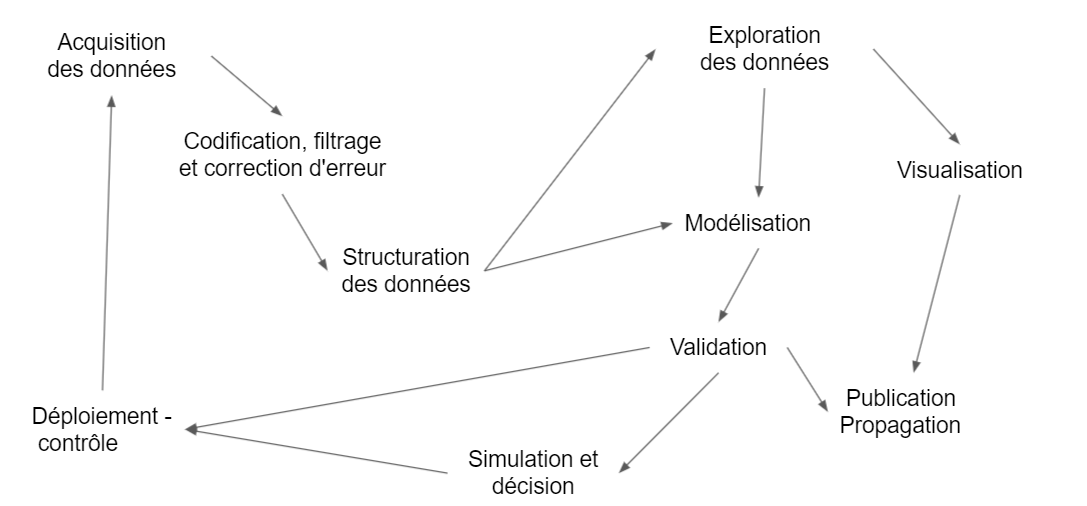
\includegraphics{./Images/datascience2.png}

\begin{itemize}
\tightlist
\item
  Acquisition
\item
  Codification , filtrage et correction d'erreur
\item
  Structuration des données : api, open data
\item
  Exploration
\item
  Modélisation :
\item
  validation : tests versus AB testing
\item
  Simulation et décision
\item
  Vizualisation et sensemaking
\item
  Déploiement :
\item
  Contrôle :
\item
  Publication : dash board, pdf , slide etc, webb site
\end{itemize}

\hypertarget{les-facteurs-de-duxe9veloppement-des-datasciences}{%
\section{Les facteurs de développement des datasciences}\label{les-facteurs-de-duxe9veloppement-des-datasciences}}

Ces développements sont favorisés par un environnement fertile dont trois facteurs se renforcent mutuellement.

\hypertarget{une-lingua-franca}{%
\subsection{Une lingua franca}\label{une-lingua-franca}}

histoire de r
histoire de python

\hypertarget{une-communautuxe9}{%
\subsection{Une communauté}\label{une-communautuxe9}}

Le second facteur , intimement lié au premier, est la constitution d'une large communauté de développeurs et d'utilisateurs qui se retrouvent aujourd'hui dans des plateformes de dépots (Github, Gitlab), de plateformes de type quora (StalkOverFlow), de tutoriaux, de blogs (BloggeR), de journaux (Journal of Statistical Software) et de bookdown.

Des ressources abondantes sont ainsi disponibles et facilitent la formation des chercheurs et des data scientists. Toutes les conditions sont réunies pour engendrer une effervescence créative.

\hypertarget{la-multiplication-des-sources-de-donnuxe9es.}{%
\subsection{La multiplication des sources de données.}\label{la-multiplication-des-sources-de-donnuxe9es.}}

Le troisième est la multiplication des sources de données et leur facilité d'accès. Les données privées, et en particulier celles des réseaux sociaux, même si un péage doit être payé pour accéder aux APIs, popularisent le traitement de données massives. Le mouvement des données ouvertes (open data) proposent et facilitent l'accès à des milliers de corps de données : retards de la SNCF, grand débat, le formidable travail de l'Insee, european survey etc.

\hypertarget{du-ml-uxe0-lia}{%
\section{du ML à l'IA}\label{du-ml-uxe0-lia}}

\hypertarget{prise-en-main}{%
\chapter{Prise en main}\label{prise-en-main}}

Pour démarrer :

1 - Télécharger et installer r sur le site du Comprehensive r Archive Network
2 - Télécharger et installer Rstudio.(version free)
3 - Dans le cadre de cet atelier, on adopte la méthode du rMarkdown, On recommande fortement de lire l'ouvrage de référence, même si la prise en main est très rapide. Il est désormais indispensable d'utiliser le package tidyverse et en particulier les fonctions de manipulation et de pipe de fichier de dplyr

\hypertarget{la-convention-du-rmarkdown}{%
\section{La convention du Rmarkdown}\label{la-convention-du-rmarkdown}}

Différentes manières d'interagir avec r sont possibles, dans ce manuel nous adoptions les méthodes \href{https://rmarkdown.rstudio.com/lesson-1.html}{rmarkdown}.

La première est le mode console, pour de petite opérations et un utilisateur chevronné, celà peut être commode car rapide mais très rapidement on sera amené à enregistrer les opérations dans des scripts. Mais pour produires des résultats, il faut lancer le script.

Une idée novatrice a été d'intégrer l'ensemble des élements dans un seul document : le script découpé en petits éléments : des chunks, le commentaire et l'analyse verbabe dans un format texte, et le résultat. Dans l'univers python il s'agit des carnets Jupiter, pour r c'est le rmarkdown.

C'est un dialecte du markdown générique adapté au langage r. On recommande au lecteur d'en lire \href{https://bookdown.org/yihui/rmarkdown/}{le manuel} et de le garder dans ses onglets.

Quelques éléments de base :

un document markdown est composé de plusieurs éléments

\begin{itemize}
\tightlist
\item
  Yalm dans cet entête les éléments essentiels sont définis et paramétrés
\item
  Texte : il suit les conventions de mise en forme du html :
  ** des \# pour les niveau de titres
  ** (x){[}*.html{]} pour des liens et \includegraphics{image.jpg} pour des images
  **
\item
  Les chunks sont isolé par 3 tiks au début et à la fin.
\item
  Résultats
\end{itemize}

\url{https://rmarkdown.rstudio.com/authoring_pandoc_markdown.html\#Footnotes}

On peut en réalité constituer un document complet le le publier en word, en hatml ou mieux en pdf/latex.
avec les éléments suivant

\begin{itemize}
\tightlist
\item
  bibliographie
\item
  références
\item
  liens
\item
  images
\end{itemize}

\hypertarget{lire-les-donnuxe9es}{%
\section{Lire les données}\label{lire-les-donnuxe9es}}

La première étape c'est la lecture des données. On commence par le plus simple la lecture de fichiers locaux, on jette un coup d'oeil à la diversité des formats, on introduit à la technique des accès directs bien utile pour s'assurer que les données sont bien fraiches.

\hypertarget{le-cas-usuels-des-.csv}{%
\subsection{le cas usuels des *.csv}\label{le-cas-usuels-des-.csv}}

\begin{Shaded}
\begin{Highlighting}[]
\NormalTok{df <-}\StringTok{ }\KeywordTok{read_csv}\NormalTok{(}\StringTok{"./Data/BXL_listings.csv"}\NormalTok{)}
\end{Highlighting}
\end{Shaded}

\hypertarget{la-diversituxe9-des-formats}{%
\subsection{La diversité des formats}\label{la-diversituxe9-des-formats}}

Peu de formats échappent à r, ils peuvent faire appel à des packages spécifiques

\begin{itemize}
\tightlist
\item
  excell
\item
  Json
\item
  shape et autre GIS :
\item
  les formats bibliographique : bib et ris
\end{itemize}

\hypertarget{les-accuxe8s-directs}{%
\section{Les accès directs}\label{les-accuxe8s-directs}}

Interfaces

le génie des API : ne pas se soucier de la mise à jour à chaque fois qu'on lance un calcul.

exemples :

\begin{itemize}
\tightlist
\item
  base d'archive de presse
\item
  api des réseaux sociaux
\item
  open data
\end{itemize}

\hypertarget{dplyr-pour-manipuler-les-donnuxe9es}{%
\section{\texorpdfstring{\texttt{Dplyr} pour manipuler les données}{Dplyr pour manipuler les données}}\label{dplyr-pour-manipuler-les-donnuxe9es}}

C'est un des packages essentiel de la suite tidyverse.

\hypertarget{des-pipes}{%
\subsection{Des pipes \%\textgreater\%}\label{des-pipes}}

Une grand part de l'intérêt de dplyr est de reprendre un opérateur de maggritr très utiles : le pipe : \%\textgreater\%. Celui ci permet de passer le résultats de l'opération à gauche, dans la fonction de droite.

Un exemple simple . Dans la ligne de code suivante, une première fonction lit le fichier CSV, et envoie le résultat de cette lecture dans une fonction graphique élémentaire: compter le nombre d'occurences des modalité de la variable room\_type. On reviendra longuement sur ggplot, à ce stade ce qui compte c'est de retenir le procédé.

On va très vite en donner des exemples plus variés.

\begin{Shaded}
\begin{Highlighting}[]
\NormalTok{g <-}\StringTok{ }\KeywordTok{read_csv}\NormalTok{(}\StringTok{"./Data/BXL_listings.csv"}\NormalTok{) }\OperatorTok\StringTok{ }
\StringTok{  }\KeywordTok{ggplot}\NormalTok{(}\KeywordTok{aes}\NormalTok{(}\DataTypeTok{x=}\NormalTok{price))}\OperatorTok{+}\KeywordTok{geom_histogram}\NormalTok{()}
\NormalTok{g}
\end{Highlighting}
\end{Shaded}

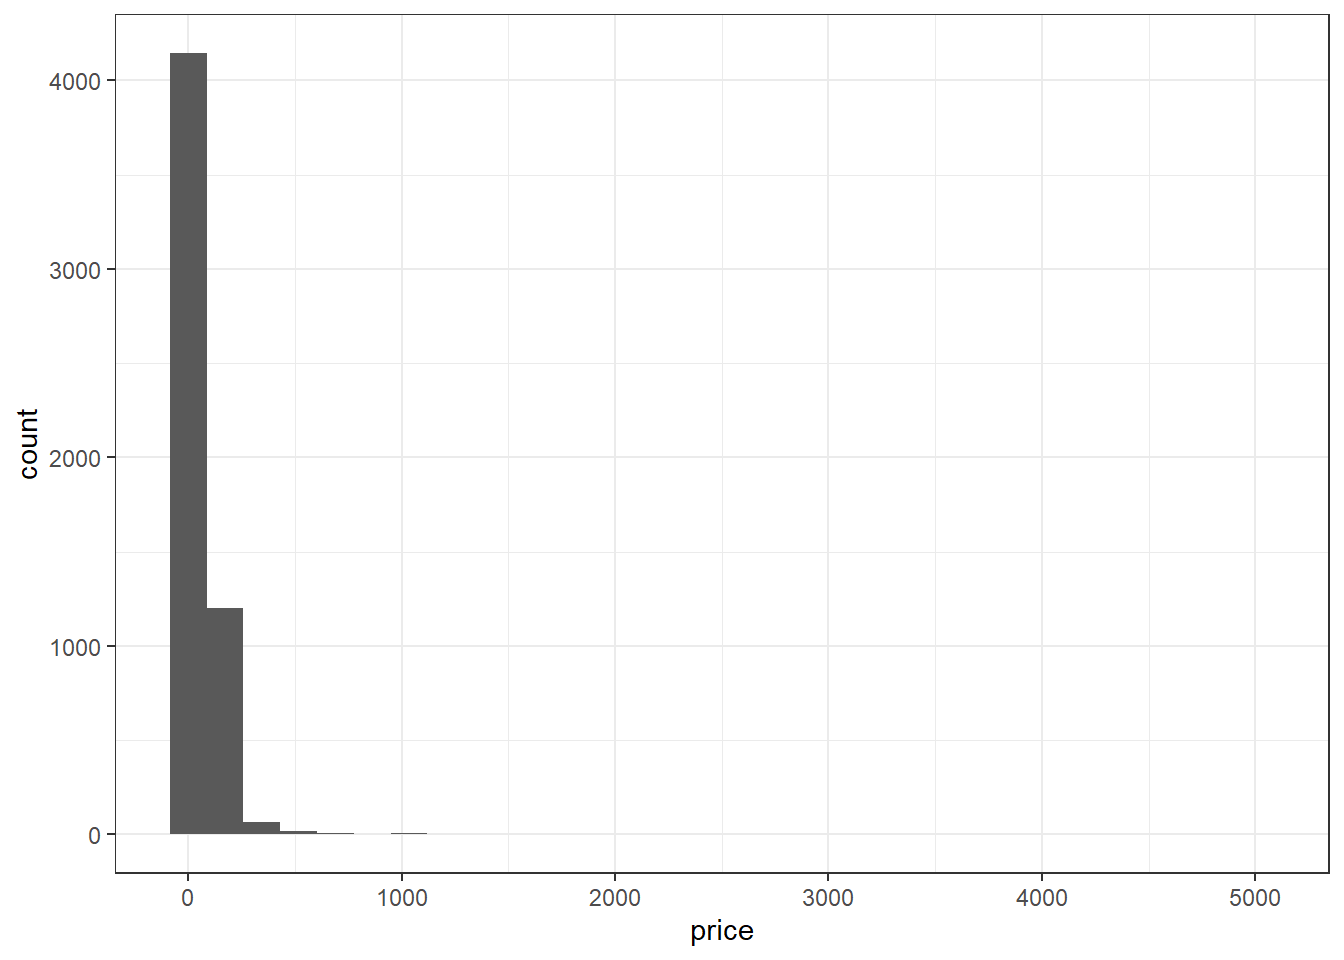
\includegraphics{bookdown-demo_files/figure-latex/203-1.pdf}

\hypertarget{des-verbes}{%
\subsection{Des verbes}\label{des-verbes}}

L'originalité de dplyr est de définir des fonctions comme des verbes. Chaque verbe désigne un type d'action. On va les examiner progressivement

et \href{http://larmarange.github.io/analyse-R/manipuler-les-donnees-avec-dplyr.html}{dplyr} qui va nous permettre de manipuler les données aisément.

Ils sont simples à comprendre : tansformer une variables, filter les obsersation selon un critère, isoler des variables, les groupper pour en calculer des résultats statistiqyes ( somme, moyenne, variance, max min etc) * les déplouer selon un format long ou les distribuer en différents critères, les fusionner enfin selon les grandes modalité du SQL)

\hypertarget{mutate}{%
\subsubsection{Mutate}\label{mutate}}

En Français c'est ``transformer''. On modifie la valeur d'une variable par une fonction plus ou moins complexe, éventuellement en ajoutant des conditions.

Dans notre exemple, faisant au plus simple, puisque la distribution est asymétrique, une transformation du prix par les log peut donner des résultats intéressants.

Et c'est le cas. On retrouve une distribution qui semble être gaussienne.

\begin{Shaded}
\begin{Highlighting}[]
\NormalTok{g <-}\StringTok{ }\KeywordTok{read_csv}\NormalTok{(}\StringTok{"./Data/BXL_listings.csv"}\NormalTok{) }\OperatorTok\StringTok{ }
\StringTok{  }\KeywordTok{mutate}\NormalTok{(}\DataTypeTok{price=}\KeywordTok{log10}\NormalTok{(price))}\OperatorTok
\StringTok{  }\KeywordTok{ggplot}\NormalTok{(}\KeywordTok{aes}\NormalTok{(}\DataTypeTok{x=}\NormalTok{price))}\OperatorTok{+}\KeywordTok{geom_histogram}\NormalTok{()}
\NormalTok{g}
\end{Highlighting}
\end{Shaded}

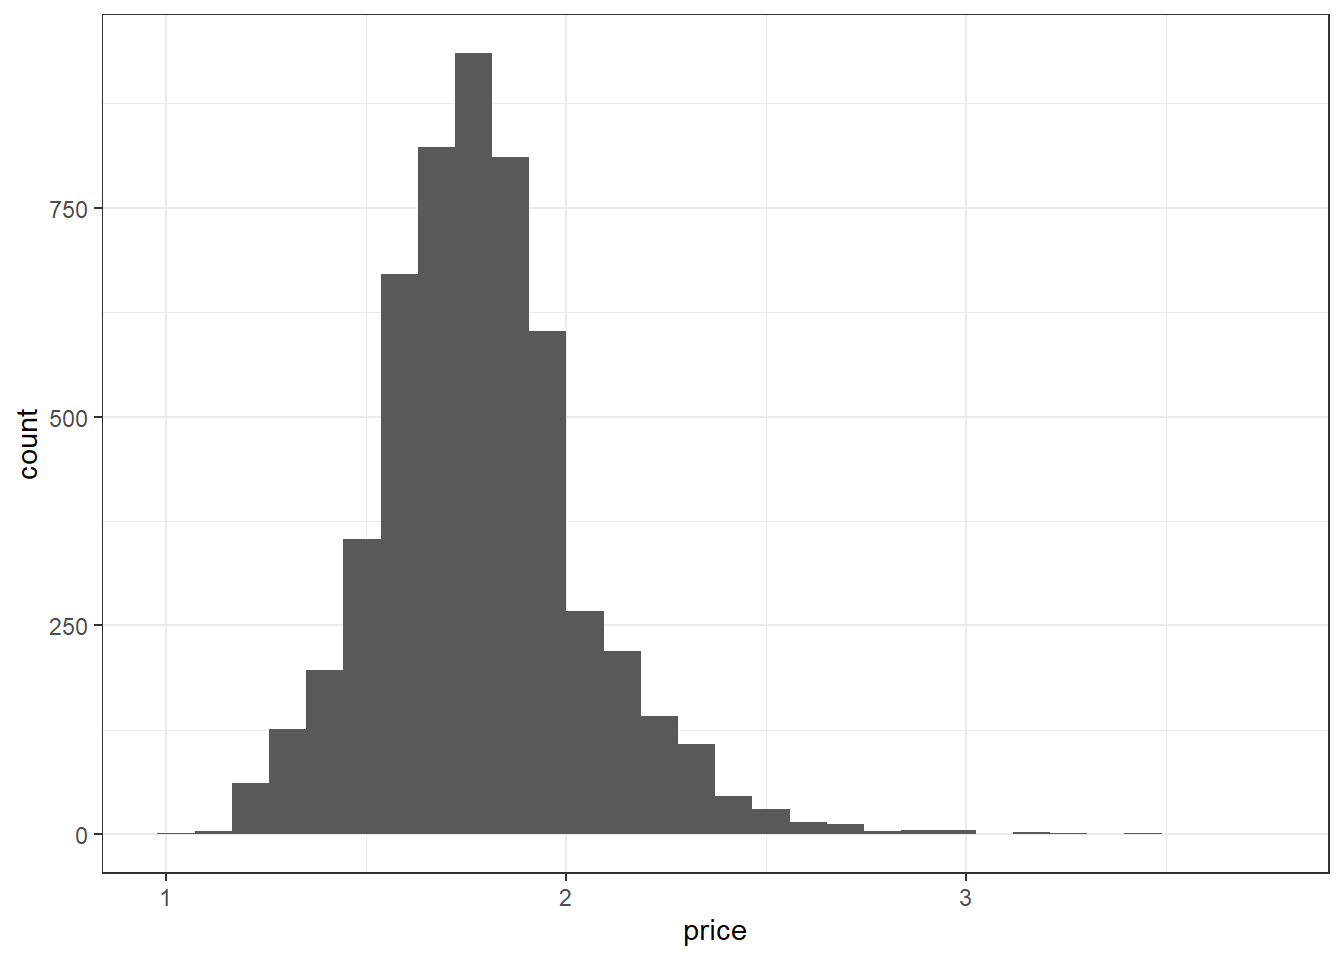
\includegraphics{bookdown-demo_files/figure-latex/204-1.pdf}

\hypertarget{filter}{%
\subsubsection{Filter}\label{filter}}

On peut voulir se concentrer sur une sous population. par exemple les chambres privées

\begin{Shaded}
\begin{Highlighting}[]
\NormalTok{g <-}\StringTok{ }\KeywordTok{read_csv}\NormalTok{(}\StringTok{"./Data/BXL_listings.csv"}\NormalTok{) }\OperatorTok\StringTok{ }
\StringTok{  }\KeywordTok{filter}\NormalTok{(room_type}\OperatorTok{==}\StringTok{"Private room"}\NormalTok{)}\OperatorTok\StringTok{ }
\StringTok{  }\CommentTok{# on note que le signe == est double, c'est pour dire que la variable prend la valeur, ou non, qui est proposée}
\StringTok{  }\KeywordTok{mutate}\NormalTok{(}\DataTypeTok{price=}\KeywordTok{log10}\NormalTok{(price))}\OperatorTok
\StringTok{  }\KeywordTok{ggplot}\NormalTok{(}\KeywordTok{aes}\NormalTok{(}\DataTypeTok{x=}\NormalTok{price))}\OperatorTok{+}\KeywordTok{geom_histogram}\NormalTok{()}
\NormalTok{g}
\end{Highlighting}
\end{Shaded}

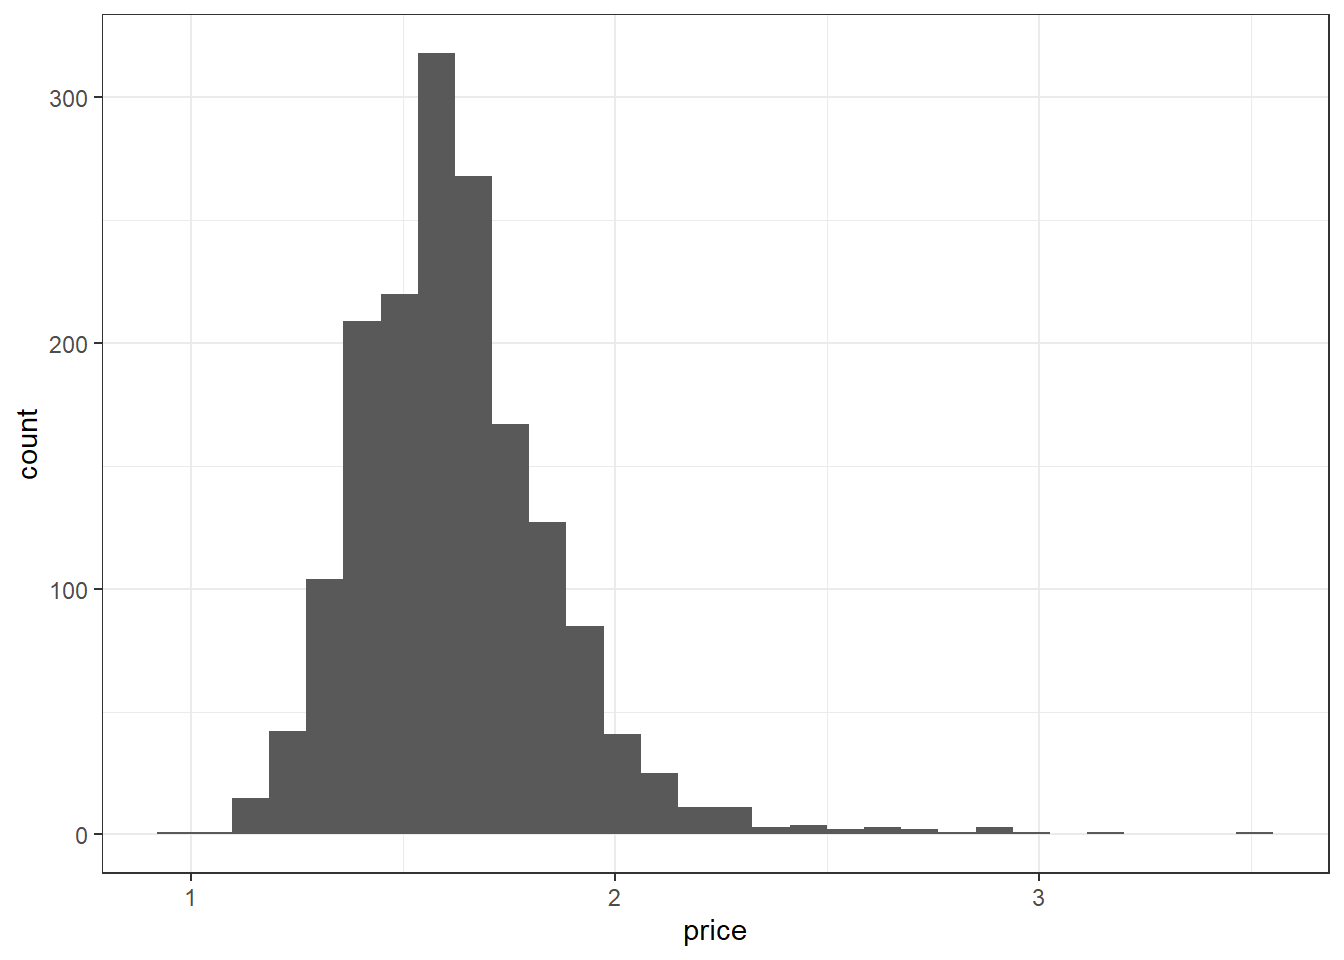
\includegraphics{bookdown-demo_files/figure-latex/205-1.pdf}
* filter

\hypertarget{select}{%
\subsubsection{select}\label{select}}

\begin{Shaded}
\begin{Highlighting}[]
\NormalTok{g <-}\StringTok{ }\KeywordTok{read_csv}\NormalTok{(}\StringTok{"./Data/BXL_listings.csv"}\NormalTok{) }\OperatorTok\StringTok{ }
\StringTok{  }\KeywordTok{filter}\NormalTok{(room_type}\OperatorTok{==}\StringTok{"Private room"}\NormalTok{)}\OperatorTok\StringTok{ }
\StringTok{  }\CommentTok{# on note que le signe == est double, c'est pour dire que la variable prend la valeur, ou non, qui est proposée}
\StringTok{  }\KeywordTok{mutate}\NormalTok{(}\DataTypeTok{price=}\KeywordTok{log10}\NormalTok{(price))}\OperatorTok
\StringTok{  }\KeywordTok{ggplot}\NormalTok{(}\KeywordTok{aes}\NormalTok{(}\DataTypeTok{x=}\NormalTok{price))}\OperatorTok{+}\KeywordTok{geom_histogram}\NormalTok{()}
\NormalTok{g}
\end{Highlighting}
\end{Shaded}

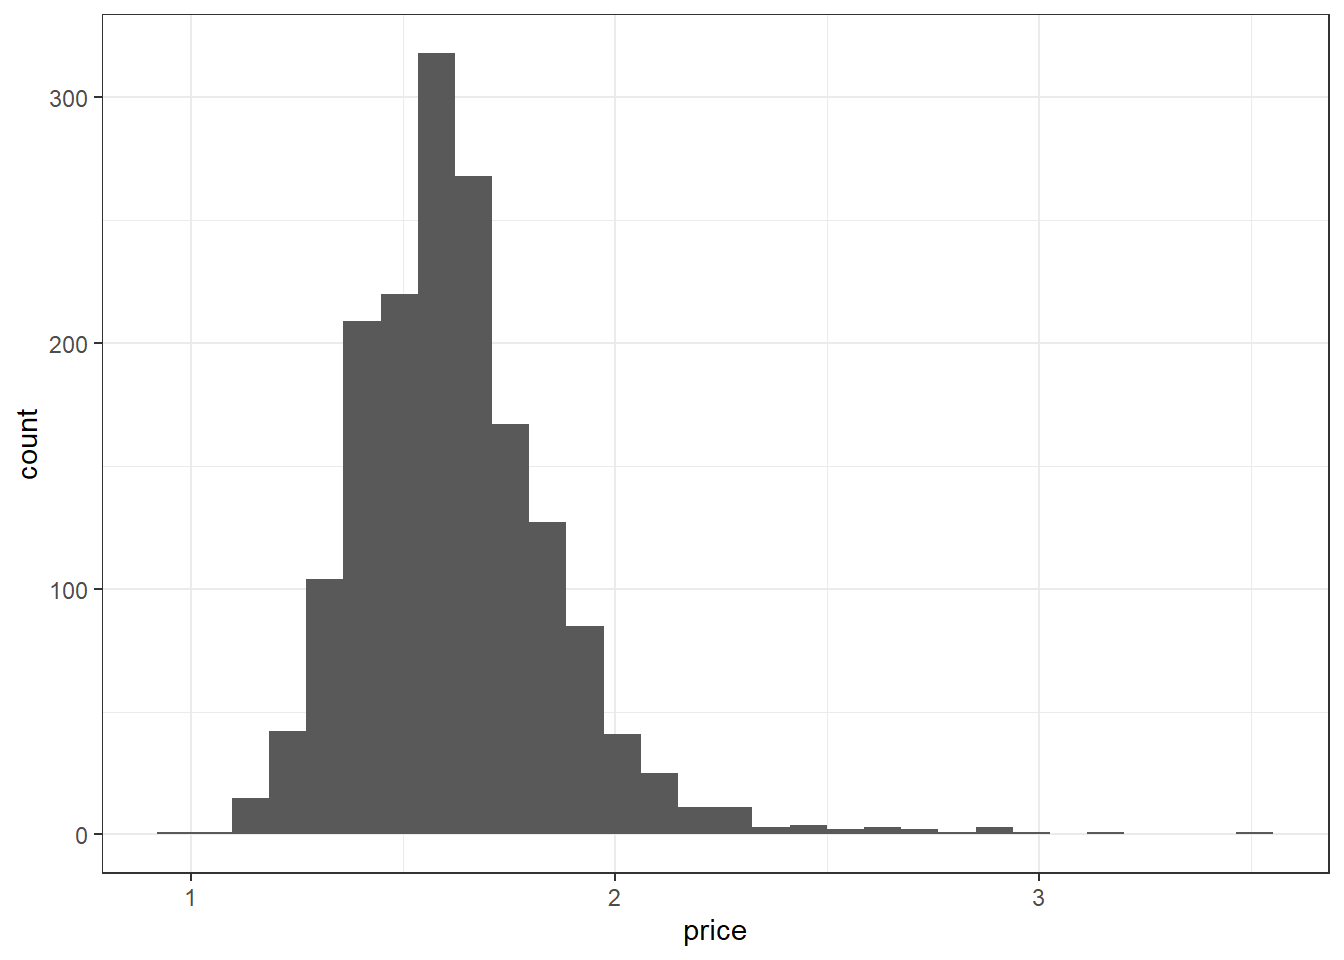
\includegraphics{bookdown-demo_files/figure-latex/206-1.pdf}

\hypertarget{group_by-et-summarize}{%
\subsubsection{Group\_by et summarize}\label{group_by-et-summarize}}

c'est une opération clé, en groupant selon les modalités d'une ou pluseirs variables, on peut construire des tableaux aggrégés.On l'associera à \texttt{summarize} qui permet de calculer les statistique aggrégé selon le groupe que l'on a définit

\begin{Shaded}
\begin{Highlighting}[]
\NormalTok{g <-}\StringTok{ }\KeywordTok{read_csv}\NormalTok{(}\StringTok{"./Data/BXL_listings.csv"}\NormalTok{)}\OperatorTok\StringTok{ }
\StringTok{  }\NormalTok{dplyr}\OperatorTok{::}\KeywordTok{select}\NormalTok{(neighbourhood, price)}\OperatorTok
\StringTok{    }\KeywordTok{group_by}\NormalTok{(neighbourhood ) }\OperatorTok\StringTok{ }
\StringTok{  }\KeywordTok{summarise}\NormalTok{(}\DataTypeTok{price=}\KeywordTok{mean}\NormalTok{(price))}\OperatorTok\StringTok{ }\CommentTok{# ce qi permet de calculer le prix moyen par quartier}
\StringTok{  }\KeywordTok{ggplot}\NormalTok{(}\KeywordTok{aes}\NormalTok{(}\DataTypeTok{x=}\NormalTok{neighbourhood, }\DataTypeTok{y=}\NormalTok{price))}\OperatorTok{+}
\StringTok{  }\KeywordTok{geom_bar}\NormalTok{(}\DataTypeTok{stat=} \StringTok{"identity"}\NormalTok{)}\OperatorTok{+}\StringTok{ }\KeywordTok{coord_flip}\NormalTok{() }\OperatorTok{+}\KeywordTok{labs}\NormalTok{(}\DataTypeTok{title=}\StringTok{"Prix moyen des Airbnb à Bruxelles"}\NormalTok{)}
\NormalTok{g}
\end{Highlighting}
\end{Shaded}

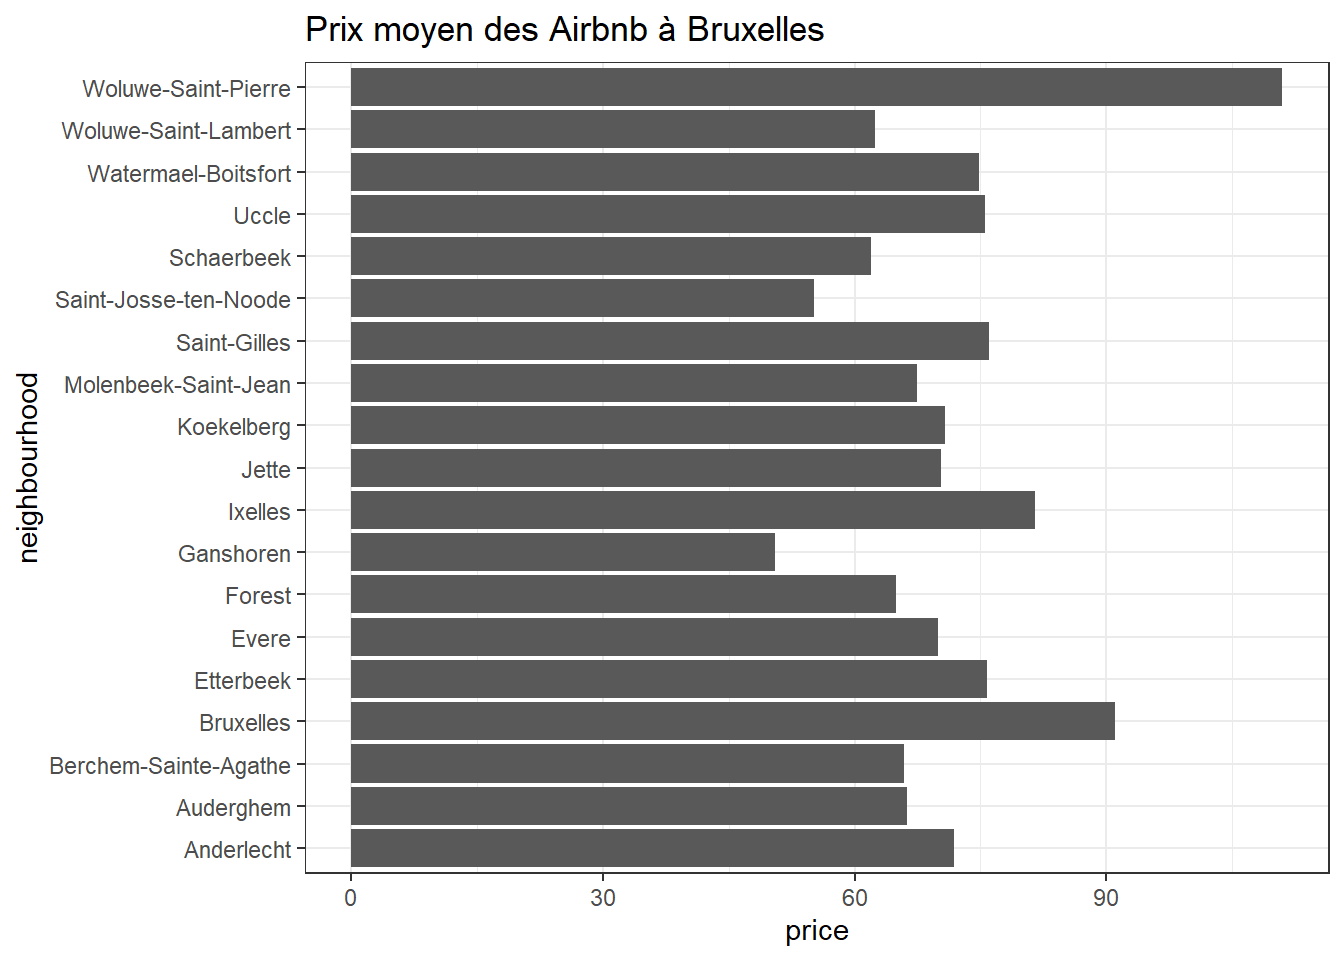
\includegraphics{bookdown-demo_files/figure-latex/207-1.pdf}

\hypertarget{gather-and-spread}{%
\subsubsection{gather and spread}\label{gather-and-spread}}

Si pour l'habitué des feuilles excell les données croisent des observations avec des variables, ce format n'est pas le seul moyuen de répsenter des données, et pas forcément le meilleurs

\hypertarget{merge}{%
\subsubsection{merge}\label{merge}}

On sera souvent amené à fabriquer des tableaux de donnée en les enrichissant d'un autre. On sera amené fusionner les données.

Le cas le plus simples est d'ajouter d'autres observation à un fichier de données, si les variables sont identitiques on peut concaténer diffrents jeux de données avec la fonction de base rbind au contraire si les observation sont les mêmes, et que seules les variables sont différentes on peut utiliser cbind. L'équivalent de DPLYR est row\_bind et column\_bind

mais très souvent on sera dans des cas différents et la fusion des données devra suivre des index

\begin{figure}
\centering
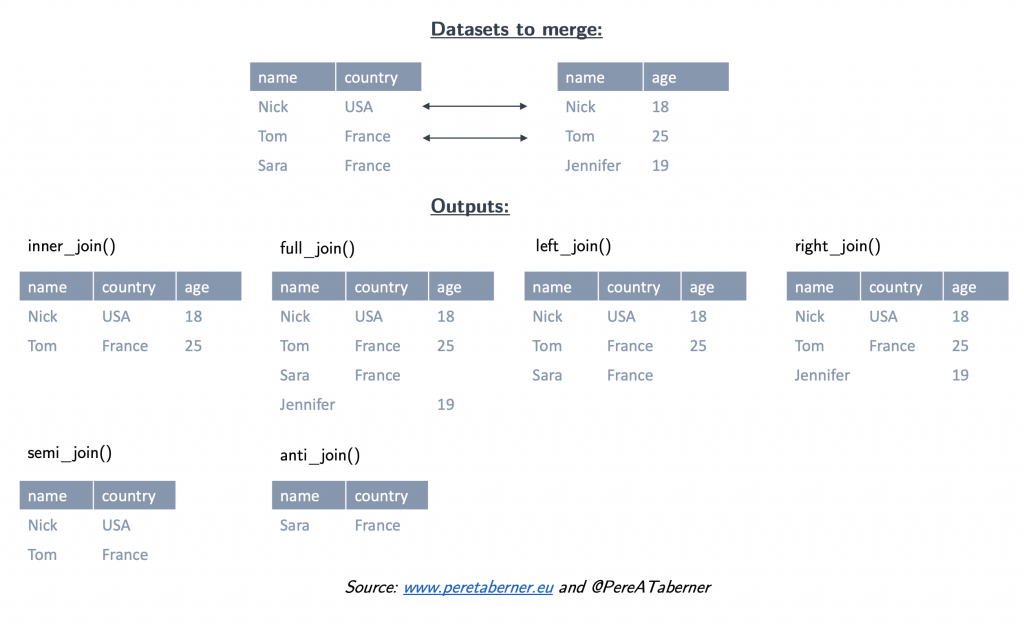
\includegraphics{./Images/merge_ex-1024x624.png}
\caption{merge}
\end{figure}

quatre types de fusion

genérale

fusion à gauche

fusion à droite

\url{https://coletl.github.io/tidy_intro/lessons/dplyr_join/dplyr_join.html}

\hypertarget{pour-aller-plus-loin}{%
\section{Pour aller plus loin}\label{pour-aller-plus-loin}}

On engage le lecteur à poursuivre avec

\begin{itemize}
\tightlist
\item
  le bookdown au-delà du markdown
\item
  une théorie des tidy data
\end{itemize}

\hypertarget{etude-de-cas}{%
\section{Etude de cas}\label{etude-de-cas}}

Le plan de recodage d'un jeu de données qu'on va employer dans les chapitre suivant. Il s'appuie sur le langage de base.

Un excercice peut être de le réécrire avec dplyr.

\begin{Shaded}
\begin{Highlighting}[]
\NormalTok{df<-}\KeywordTok{readRDS}\NormalTok{(}\StringTok{"./data/trustFrAll.rds"}\NormalTok{)}

\CommentTok{#quelques recodages}
\CommentTok{#on renomme pour plus de clarte}
\KeywordTok{names}\NormalTok{(df)[}\KeywordTok{names}\NormalTok{(df)}\OperatorTok{==}\StringTok{"trstun"}\NormalTok{] <-}\StringTok{ "NationsUnies"} 
\KeywordTok{names}\NormalTok{(df)[}\KeywordTok{names}\NormalTok{(df)}\OperatorTok{==}\StringTok{"trstep"}\NormalTok{] <-}\StringTok{ "ParlementEurop"} 
\KeywordTok{names}\NormalTok{(df)[}\KeywordTok{names}\NormalTok{(df)}\OperatorTok{==}\StringTok{"trstlgl"}\NormalTok{] <-}\StringTok{ "Justice"} 
\KeywordTok{names}\NormalTok{(df)[}\KeywordTok{names}\NormalTok{(df)}\OperatorTok{==}\StringTok{"trstplc"}\NormalTok{] <-}\StringTok{ "Police"} 
\KeywordTok{names}\NormalTok{(df)[}\KeywordTok{names}\NormalTok{(df)}\OperatorTok{==}\StringTok{"trstplt"}\NormalTok{] <-}\StringTok{ "Politiques"} 
\KeywordTok{names}\NormalTok{(df)[}\KeywordTok{names}\NormalTok{(df)}\OperatorTok{==}\StringTok{"trstprl"}\NormalTok{] <-}\StringTok{"Parlement"} 
\KeywordTok{names}\NormalTok{(df)[}\KeywordTok{names}\NormalTok{(df)}\OperatorTok{==}\StringTok{"trstprt"}\NormalTok{] <-}\StringTok{ "Partis"}
\KeywordTok{names}\NormalTok{(df)[}\KeywordTok{names}\NormalTok{(df)}\OperatorTok{==}\StringTok{"pplhlp"}\NormalTok{] <-}\StringTok{ "help"}
\KeywordTok{names}\NormalTok{(df)[}\KeywordTok{names}\NormalTok{(df)}\OperatorTok{==}\StringTok{"pplfair"}\NormalTok{] <-}\StringTok{ "fair"}
\KeywordTok{names}\NormalTok{(df)[}\KeywordTok{names}\NormalTok{(df)}\OperatorTok{==}\StringTok{"ppltrst"}\NormalTok{] <-}\StringTok{ "trust"}

\CommentTok{#on construit les scores de confiance }
\NormalTok{df<-df }\OperatorTok\StringTok{ }
\StringTok{  }\KeywordTok{mutate}\NormalTok{(}\DataTypeTok{trust_institut=}\NormalTok{(Partis}\OperatorTok{+}\NormalTok{Parlement}\OperatorTok{+}\NormalTok{Politiques}\OperatorTok{+}\NormalTok{Police}\OperatorTok{+}\NormalTok{Justice}\OperatorTok{+}\NormalTok{NationsUnies}\OperatorTok{+}\NormalTok{ParlementEurop)}\OperatorTok{*}\DecValTok{10}\OperatorTok{/}\DecValTok{7}\NormalTok{,}\DataTypeTok{trust_interpersonnel=}\NormalTok{(help}\OperatorTok{+}\NormalTok{fair}\OperatorTok{+}\NormalTok{trust)}\OperatorTok{*}\DecValTok{10}\OperatorTok{/}\DecValTok{3}\NormalTok{)}
\NormalTok{df}\OperatorTok{$}\NormalTok{Year<-}\DecValTok{2000}
\CommentTok{#recodage des variables independantes}
\NormalTok{df}\OperatorTok{$}\NormalTok{Year[df}\OperatorTok{$}\NormalTok{essround}\OperatorTok{==}\DecValTok{1}\NormalTok{]<-}\DecValTok{2002}
\NormalTok{df}\OperatorTok{$}\NormalTok{Year[df}\OperatorTok{$}\NormalTok{essround}\OperatorTok{==}\DecValTok{2}\NormalTok{]<-}\DecValTok{2004}
\NormalTok{df}\OperatorTok{$}\NormalTok{Year[df}\OperatorTok{$}\NormalTok{essround}\OperatorTok{==}\DecValTok{3}\NormalTok{]<-}\DecValTok{2006}
\NormalTok{df}\OperatorTok{$}\NormalTok{Year[df}\OperatorTok{$}\NormalTok{essround}\OperatorTok{==}\DecValTok{4}\NormalTok{]<-}\DecValTok{2008}
\NormalTok{df}\OperatorTok{$}\NormalTok{Year[df}\OperatorTok{$}\NormalTok{essround}\OperatorTok{==}\DecValTok{5}\NormalTok{]<-}\DecValTok{2010}
\NormalTok{df}\OperatorTok{$}\NormalTok{Year[df}\OperatorTok{$}\NormalTok{essround}\OperatorTok{==}\DecValTok{6}\NormalTok{]<-}\DecValTok{2012}
\NormalTok{df}\OperatorTok{$}\NormalTok{Year[df}\OperatorTok{$}\NormalTok{essround}\OperatorTok{==}\DecValTok{7}\NormalTok{]<-}\DecValTok{2014}
\NormalTok{df}\OperatorTok{$}\NormalTok{Year[df}\OperatorTok{$}\NormalTok{essround}\OperatorTok{==}\DecValTok{8}\NormalTok{]<-}\DecValTok{2016}
\NormalTok{df}\OperatorTok{$}\NormalTok{Year[df}\OperatorTok{$}\NormalTok{essround}\OperatorTok{==}\DecValTok{9}\NormalTok{]<-}\DecValTok{2018}
\NormalTok{df}\OperatorTok{$}\NormalTok{Year<-}\KeywordTok{as.factor}\NormalTok{(df}\OperatorTok{$}\NormalTok{Year) }

\NormalTok{df}\OperatorTok{$}\NormalTok{OP<-}\StringTok{" "}
\CommentTok{#ggplot(df,aes(x=lrscale))+geom_histogram()}
\NormalTok{df}\OperatorTok{$}\NormalTok{OP[df}\OperatorTok{$}\NormalTok{lrscale}\OperatorTok{==}\DecValTok{0}\NormalTok{] <-}\StringTok{ "Extrême gauche"} 
\NormalTok{df}\OperatorTok{$}\NormalTok{OP[df}\OperatorTok{$}\NormalTok{lrscale}\OperatorTok{==}\DecValTok{1}\NormalTok{] <-}\StringTok{ "Gauche"} 
\NormalTok{df}\OperatorTok{$}\NormalTok{OP[df}\OperatorTok{$}\NormalTok{lrscale}\OperatorTok{==}\DecValTok{2}\NormalTok{] <-}\StringTok{ "Gauche"} 
\NormalTok{df}\OperatorTok{$}\NormalTok{OP[df}\OperatorTok{$}\NormalTok{lrscale}\OperatorTok{==}\DecValTok{3}\NormalTok{] <-}\StringTok{ "Centre Gauche"} 
\NormalTok{df}\OperatorTok{$}\NormalTok{OP[df}\OperatorTok{$}\NormalTok{lrscale}\OperatorTok{==}\DecValTok{4}\NormalTok{] <-}\StringTok{ "Centre Gauche"} 
\NormalTok{df}\OperatorTok{$}\NormalTok{OP[df}\OperatorTok{$}\NormalTok{lrscale}\OperatorTok{==}\DecValTok{5}\NormalTok{] <-}\StringTok{ "Ni G ni D"} 
\NormalTok{df}\OperatorTok{$}\NormalTok{OP[df}\OperatorTok{$}\NormalTok{lrscale}\OperatorTok{==}\DecValTok{6}\NormalTok{] <-}\StringTok{ "Centre Droit"} 
\NormalTok{df}\OperatorTok{$}\NormalTok{OP[df}\OperatorTok{$}\NormalTok{lrscale}\OperatorTok{==}\DecValTok{7}\NormalTok{] <-}\StringTok{ "Centre Droit"} 
\NormalTok{df}\OperatorTok{$}\NormalTok{OP[df}\OperatorTok{$}\NormalTok{lrscale}\OperatorTok{==}\DecValTok{8}\NormalTok{] <-}\StringTok{ "Droite"} 
\NormalTok{df}\OperatorTok{$}\NormalTok{OP[df}\OperatorTok{$}\NormalTok{lrscale}\OperatorTok{==}\DecValTok{9}\NormalTok{] <-}\StringTok{ "Droite"} 
\NormalTok{df}\OperatorTok{$}\NormalTok{OP[df}\OperatorTok{$}\NormalTok{lrscale}\OperatorTok{==}\DecValTok{10}\NormalTok{] <-}\StringTok{ "Extrême droite"} 
\CommentTok{#la ligne suivante est pour ordonner les modalités de la variables}
\NormalTok{df}\OperatorTok{$}\NormalTok{OP<-}\KeywordTok{factor}\NormalTok{(df}\OperatorTok{$}\NormalTok{OP,}\DataTypeTok{levels=}\KeywordTok{c}\NormalTok{(}\StringTok{"Extrême droite"}\NormalTok{,}\StringTok{"Droite"}\NormalTok{,}\StringTok{"Centre Droit"}\NormalTok{,}\StringTok{"Ni G ni D"}\NormalTok{,}\StringTok{"Centre Gauche"}\NormalTok{,}\StringTok{"Gauche"}\NormalTok{,}\StringTok{"Extrême gauche"}\NormalTok{))}


\NormalTok{df}\OperatorTok{$}\NormalTok{revenu<-}\StringTok{" "}
\NormalTok{df}\OperatorTok{$}\NormalTok{revenu[df}\OperatorTok{$}\NormalTok{hincfel}\OperatorTok{>}\DecValTok{4}\NormalTok{] <-}\StringTok{ }\OtherTok{NA}
\NormalTok{df}\OperatorTok{$}\NormalTok{revenu[df}\OperatorTok{$}\NormalTok{hincfel}\OperatorTok{==}\DecValTok{1}\NormalTok{] <-}\StringTok{ "Vie confortable"} 
\NormalTok{df}\OperatorTok{$}\NormalTok{revenu[df}\OperatorTok{$}\NormalTok{hincfel}\OperatorTok{==}\DecValTok{2}\NormalTok{] <-}\StringTok{ "Se débrouille avec son revenu"} 
\NormalTok{df}\OperatorTok{$}\NormalTok{revenu[df}\OperatorTok{$}\NormalTok{hincfel}\OperatorTok{==}\DecValTok{3}\NormalTok{] <-}\StringTok{ "Revenu insuffisant"} 
\NormalTok{df}\OperatorTok{$}\NormalTok{revenu[df}\OperatorTok{$}\NormalTok{hincfel}\OperatorTok{==}\DecValTok{4}\NormalTok{] <-}\StringTok{ "Revenu très insuffisant"} 
\NormalTok{df}\OperatorTok{$}\NormalTok{revenu<-}\KeywordTok{factor}\NormalTok{(df}\OperatorTok{$}\NormalTok{revenu,}\DataTypeTok{levels=}\KeywordTok{c}\NormalTok{(}\StringTok{"Vie confortable"}\NormalTok{,}\StringTok{"Se débrouille avec son revenu"}\NormalTok{,}\StringTok{"Revenu insuffisant"}\NormalTok{,}\StringTok{"Revenu très insuffisant"}\NormalTok{))}

\NormalTok{df}\OperatorTok{$}\NormalTok{habitat<-}\StringTok{" "}

\NormalTok{df}\OperatorTok{$}\NormalTok{habitat[df}\OperatorTok{$}\NormalTok{domicil}\OperatorTok{==}\DecValTok{1}\NormalTok{]<-}\StringTok{ "Big city"}
\NormalTok{df}\OperatorTok{$}\NormalTok{habitat[df}\OperatorTok{$}\NormalTok{domicil}\OperatorTok{==}\DecValTok{2}\NormalTok{]<-}\StringTok{"Suburbs"}
\NormalTok{df}\OperatorTok{$}\NormalTok{habitat[df}\OperatorTok{$}\NormalTok{domicil}\OperatorTok{==}\DecValTok{3}\NormalTok{]<-}\StringTok{"Town"}
\NormalTok{df}\OperatorTok{$}\NormalTok{habitat[df}\OperatorTok{$}\NormalTok{domicil}\OperatorTok{==}\DecValTok{4}\NormalTok{]<-}\StringTok{"Village"}
\NormalTok{df}\OperatorTok{$}\NormalTok{habitat[df}\OperatorTok{$}\NormalTok{domicil}\OperatorTok{==}\DecValTok{5}\NormalTok{]<-}\StringTok{"Countryside"}
\NormalTok{df}\OperatorTok{$}\NormalTok{habitat<-}\KeywordTok{factor}\NormalTok{(df}\OperatorTok{$}\NormalTok{habitat,}\DataTypeTok{levels=}\KeywordTok{c}\NormalTok{(}\StringTok{"Big city"}\NormalTok{,}\StringTok{"Suburbs"}\NormalTok{,}\StringTok{"Town"}\NormalTok{,}\StringTok{"Village"}\NormalTok{,}\StringTok{"Countryside"}\NormalTok{))}

\NormalTok{df}\OperatorTok{$}\NormalTok{genre<-}\StringTok{" "}

\NormalTok{df}\OperatorTok{$}\NormalTok{genre[df}\OperatorTok{$}\NormalTok{gndr}\OperatorTok{==}\DecValTok{1}\NormalTok{]<-}\StringTok{"H"}
\NormalTok{df}\OperatorTok{$}\NormalTok{genre[df}\OperatorTok{$}\NormalTok{gndr}\OperatorTok{==}\DecValTok{2}\NormalTok{]<-}\StringTok{"F"}

\NormalTok{df}\OperatorTok{$}\NormalTok{age<-}\StringTok{" "}

\NormalTok{df}\OperatorTok{$}\NormalTok{age[df}\OperatorTok{$}\NormalTok{agea}\OperatorTok{<}\DecValTok{26}\NormalTok{]<-}\StringTok{"25<"}
\NormalTok{df}\OperatorTok{$}\NormalTok{age[df}\OperatorTok{$}\NormalTok{agea}\OperatorTok{>}\DecValTok{25} \OperatorTok{&}\StringTok{ }\NormalTok{df}\OperatorTok{$}\NormalTok{agea}\OperatorTok{<}\DecValTok{36}\NormalTok{]<-}\StringTok{"26-35"}
\NormalTok{df}\OperatorTok{$}\NormalTok{age[df}\OperatorTok{$}\NormalTok{agea}\OperatorTok{>}\DecValTok{35} \OperatorTok{&}\StringTok{ }\NormalTok{df}\OperatorTok{$}\NormalTok{agea}\OperatorTok{<}\DecValTok{46}\NormalTok{]<-}\StringTok{"36-45"}
\NormalTok{df}\OperatorTok{$}\NormalTok{age[df}\OperatorTok{$}\NormalTok{agea}\OperatorTok{>}\DecValTok{45} \OperatorTok{&}\StringTok{ }\NormalTok{df}\OperatorTok{$}\NormalTok{agea}\OperatorTok{<}\DecValTok{66}\NormalTok{]<-}\StringTok{"46-65"}
\NormalTok{df}\OperatorTok{$}\NormalTok{age[df}\OperatorTok{$}\NormalTok{agea}\OperatorTok{>}\DecValTok{65} \OperatorTok{&}\StringTok{ }\NormalTok{df}\OperatorTok{$}\NormalTok{agea}\OperatorTok{<}\DecValTok{76}\NormalTok{]<-}\StringTok{"66-75"}
\NormalTok{df}\OperatorTok{$}\NormalTok{age[df}\OperatorTok{$}\NormalTok{agea}\OperatorTok{>}\DecValTok{75}\NormalTok{]<-}\StringTok{"75>"}
\NormalTok{df}\OperatorTok{$}\NormalTok{age<-}\KeywordTok{factor}\NormalTok{(df}\OperatorTok{$}\NormalTok{age,}\DataTypeTok{levels=}\KeywordTok{c}\NormalTok{(}\StringTok{"25<"}\NormalTok{,}\StringTok{"26-35"}\NormalTok{,}\StringTok{"36-45"}\NormalTok{,}\StringTok{"46-65"}\NormalTok{,}\StringTok{"66-75"}\NormalTok{, }\StringTok{"75>"}\NormalTok{))}

\KeywordTok{saveRDS}\NormalTok{(df, }\StringTok{"./data/dfTrust.rds)"}\NormalTok{)}
\end{Highlighting}
\end{Shaded}

\hypertarget{une-introduction-uxe0-ggplot}{%
\chapter{Une introduction à ggplot}\label{une-introduction-uxe0-ggplot}}

Nous avons appris à lire des données, à les manipuler, nous avons le droit d'être pressé de les représenter de manière immédiatement lisible, par des dataviz.

On présente d'abord rapidement le concept de grammaire des graphiques

On se cncentre ensuite sur un cas d'étude

On décline.

\hypertarget{la-grammaire-des-graphiques}{%
\section{La grammaire des graphiques}\label{la-grammaire-des-graphiques}}

C'est sans doute une des percées conceptuelles laplus intéressante des datasciences. La représentation graphhiques des données fait l'objet à la fois d'une explosion créative mais aussi d'une synthèse théorique. C'est l'apport de la grammaire des graphiques.

Ces outils s'appuient sur l'idée de \href{https://www.goodreads.com/book/show/2549408.The_Grammar_of_Graphics}{grammaire des graphiques}. En voici un \href{https://cfss.uchicago.edu/notes/grammar-of-graphics/}{clair résumé}.En français il y a toujours le \href{http://larmarange.github.io/analyse-R/intro-ggplot2.html}{larmarange}

\hypertarget{un-moduxe8le-en-couche}{%
\subsection{Un modèle en couche}\label{un-moduxe8le-en-couche}}

Celle-ci met un ordre dans les éléments qui composent un graphique et les superpose.

\begin{figure}
\centering

\includegraphics{./Images/graphiclayers.png}
\caption{layers}
\end{figure}

\begin{itemize}
\tightlist
\item
  l'aesthetic definit les éléments que l'on veut représenter : ce qu'on met en abscisse, ce qu'on met en ordonnné, les groupes que l'on veut distinguer.
\item
  la geométrie (geom\_x)qui définit la forme de représentation
\item
  les échelles (scale\_x)
\item
  Labelisation (labs)
\item
  les templates
\end{itemize}

ggplot est construit selon cette structure. Voici le \href{https://ggplot2-book.org/}{book de référence}

, qui est au centre de ce cours. On aura besoin de manière assez systématique de manipuler les données avant de les représenter, \href{http://larmarange.github.io/analyse-R/manipuler-les-donnees-avec-dplyr.html}{dplyr} nous permet de le faire aisément.

\hypertarget{une-typologie-des-repruxe9sentations}{%
\subsection{Une typologie des représentations}\label{une-typologie-des-repruxe9sentations}}

Un point de départ fondamental est la \href{https://www.r-graph-gallery.com/}{gallery de ggplot},, elle présente de manière synthétique toute les types de figures qui peuvent être présentées. Avec du code facilement reproductible.

Une classification simple

\begin{itemize}
\tightlist
\item
  Analyse univariée
\item
  Analyse bi variée
\item
  Analyse multivariée
  ** les variables sont quantitatives : on analyse des matrices de corrélations
  ** les variables sont qualitatives : on analyse des tableaux croisés
\item
  Analyse geospatiale
\item
  Analyse de réseaux
\item
  analyse d'arbres
\item
  Diagramme de flux
\end{itemize}

\hypertarget{lesthuxe9tique}{%
\subsection{L'esthétique}\label{lesthuxe9tique}}

L'ésthétique du diagramme dépends de ses lay out et de ses couleurs

\hypertarget{quelques-templates}{%
\subsubsection{Quelques templates}\label{quelques-templates}}

\hypertarget{lart-des-palettes}{%
\subsubsection{l'art des palettes}\label{lart-des-palettes}}

L'art des couleurs tient dans les palettes on aimera celles de Wes Anderson, on peut adorer fishualize. on trouvera

\hypertarget{une-uxe9tude-de-cas}{%
\section{Une étude de cas}\label{une-uxe9tude-de-cas}}

Les données sont extraites de l'ESS, une sélection est disponible \href{}{ici}. Elle couvre les 9 vagues et concernent la France et L'Allemagne. Les variables dépendantes (celles que l'on veut étudier et expliquer) sont les 9 items de la confiance, les variable considérées comme indépendantes (ou explicatives) sont une sélection de variables socio-démographiques : âge, genre, perception du pouvoir d'achat, orientation politique, type d'habitat.

On fait quelques opérations de recodage et on renomme les variables avoir une lecture plus aisée des variables et de leurs catégories.

On appele au début les bibliothèques. ggplot - dont voici le \href{https://ggplot2-book.org/}{book de référence}, qui est au centre de ce cours,

\hypertarget{analyse-univariuxe9e}{%
\section{Analyse univariée}\label{analyse-univariuxe9e}}

L'analyse univarié, comme son nom l'indique, ne s'intéresse qu'à une seule variable. Celle-ci peut être \textbf{quantitative} ou \textbf{qualitative} etne comporter qu'un nombre limité de modalités entre lesquels aucune comparaison de grandeur ne peut être faite. Les premières ont le plus souvent dans r un format numeric, les autres correspondent au format \emph{factor}.

\hypertarget{le-cas-des-variables-quantitatives}{%
\subsection{Le cas des variables quantitatives}\label{le-cas-des-variables-quantitatives}}

Les variables quantitatives décrivent une variable dont les valeurs décrivent les quantités d'une grandeur. Elle peuvent être discrètes (dénombrement du d'un nombre d'unités) - le nombre d'habitant), ou continue (le nombre de km parcourus). l'\textbf{histogramme} est l'outil de base pour représenter la distribution d'une telle variable. Il représente pour des intervalles de valeurs donnés, la fréquence des observations.

Sa syntaxe simple comporte d'abord la définition de la variable et de la source de données, puis une des ``géométrie'' de ggplot : la fonction geom\_histogram. Dans notre exemple, on va représenter le score de confiance institutionnelle pour la France en se concentrant sur la dernière vague d'enquête.

\begin{Shaded}
\begin{Highlighting}[]
\CommentTok{#On charge le fichier recodé à la fin du chapitre précédent}
\NormalTok{df<-}\KeywordTok{readRDS}\NormalTok{(}\StringTok{"./data/dfTrust.rds)"}\NormalTok{)}

\CommentTok{#filtrage sur 2018 et la France.}

\NormalTok{foo<-df}\OperatorTok\KeywordTok{filter}\NormalTok{(Year}\OperatorTok{==}\StringTok{"2018"} \OperatorTok{&}\StringTok{ }\NormalTok{cntry}\OperatorTok{==}\StringTok{"FR"} \OperatorTok{&}\StringTok{ }\OperatorTok{!}\KeywordTok{is.na}\NormalTok{(trust_institut))}

\CommentTok{# on stocke le diagramme dans l'objet g00, pour le réutiliser ultérieurement et pouvoir le compléter.}
\NormalTok{g00<-}\KeywordTok{ggplot}\NormalTok{(foo,}\KeywordTok{aes}\NormalTok{(}\DataTypeTok{x=}\NormalTok{trust_institut))}\OperatorTok{+}
\StringTok{  }\KeywordTok{geom_histogram}\NormalTok{()}
\NormalTok{g00}
\end{Highlighting}
\end{Shaded}

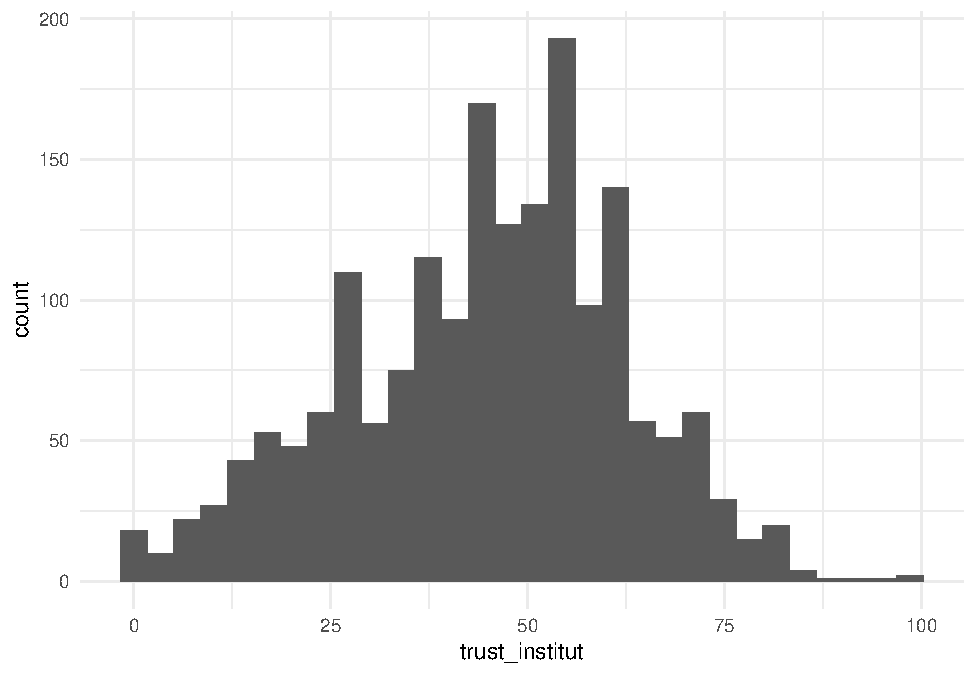
\includegraphics{bookdown-demo_files/figure-latex/302-1.pdf}

On va améliorer l'aspect en

\begin{enumerate}
\def\labelenumi{\alph{enumi})}
\tightlist
\item
  modifiant la couleur et la largeur des barres,
\item
  ajoutant un thème,
\item
  en précisant les éléments textuels (titres, label)
\item
  en calculcant et en représentant la valeur moyenne.
\end{enumerate}

\begin{Shaded}
\begin{Highlighting}[]
\CommentTok{#on calcule la moyenne}
\NormalTok{moy=}\KeywordTok{mean}\NormalTok{(foo}\OperatorTok{$}\NormalTok{trust_institut, }\DataTypeTok{na.rm=}\OtherTok{TRUE}\NormalTok{)}

\CommentTok{#avec tous les éléments}
\NormalTok{g01 <-}\KeywordTok{ggplot}\NormalTok{(foo,}\KeywordTok{aes}\NormalTok{(}\DataTypeTok{x=}\NormalTok{trust_institut))}\OperatorTok{+}
\StringTok{  }\KeywordTok{geom_histogram}\NormalTok{(}\DataTypeTok{binwidth=}\DecValTok{5}\NormalTok{,}\DataTypeTok{fill=}\StringTok{"pink"}\NormalTok{)}\OperatorTok{+}
\StringTok{  }\KeywordTok{labs}\NormalTok{(}\DataTypeTok{title=} \StringTok{"Distribution de la confiance institutionnelle"}\NormalTok{, }
       \DataTypeTok{subtitle=} \KeywordTok{paste0}\NormalTok{(}\StringTok{"moyenne = "}\NormalTok{,}\KeywordTok{round}\NormalTok{(moy,}\DecValTok{2}\NormalTok{)),}
       \DataTypeTok{caption=}\StringTok{"ESS2002-2018"}\NormalTok{,}
       \DataTypeTok{y=} \StringTok{"frequence"}\NormalTok{,}
       \DataTypeTok{x=}\StringTok{"confiance (index de 0 à 100)"}\NormalTok{) }\OperatorTok{+}
\StringTok{    }\KeywordTok{geom_vline}\NormalTok{(}\DataTypeTok{xintercept=}\NormalTok{moy, }\DataTypeTok{color=}\StringTok{"red"}\NormalTok{,}\DataTypeTok{size=}\FloatTok{1.5}\NormalTok{)}


\NormalTok{g01}
\end{Highlighting}
\end{Shaded}

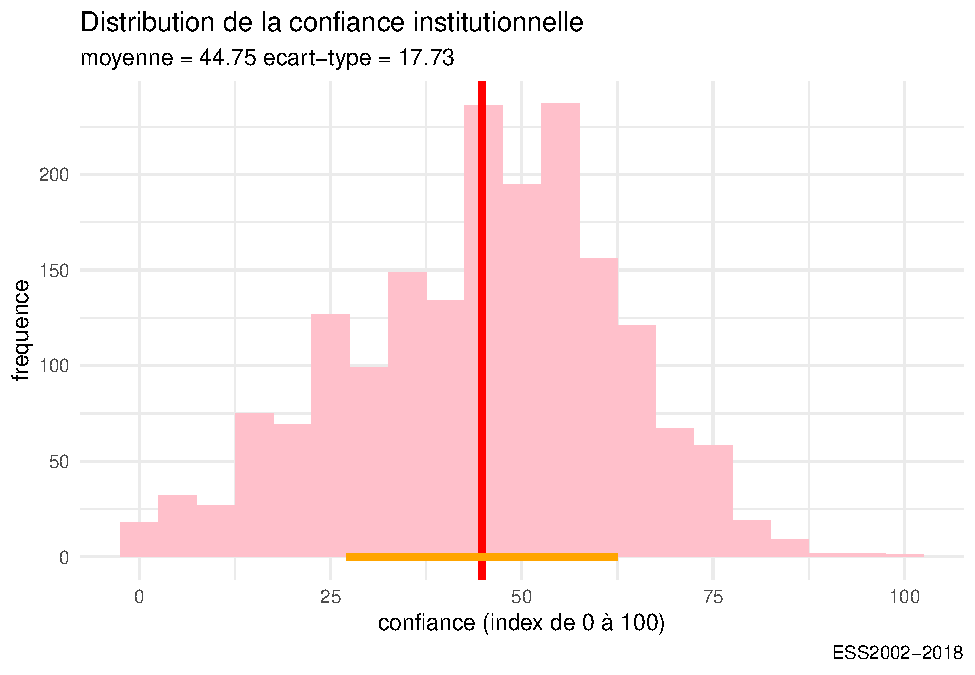
\includegraphics{bookdown-demo_files/figure-latex/303-1.pdf}

diagramme de densité : Au lieu de représenter les effectifs, on ramène l'effectif total à 1.

\begin{Shaded}
\begin{Highlighting}[]
\NormalTok{g04<-}\KeywordTok{ggplot}\NormalTok{(foo,}\KeywordTok{aes}\NormalTok{(}\DataTypeTok{x=}\NormalTok{trust_institut))}\OperatorTok{+}\StringTok{ }
\StringTok{  }\KeywordTok{geom_density}\NormalTok{(}\DataTypeTok{fill=}\StringTok{"pink2"}\NormalTok{) }\OperatorTok{+}
\StringTok{  }\KeywordTok{labs}\NormalTok{(}\DataTypeTok{title=} \StringTok{"Fonction de densité de probabilité"}\NormalTok{, }\DataTypeTok{caption=}\StringTok{"ESS2002-2018"}\NormalTok{,}\DataTypeTok{y=} \StringTok{"frequence"}\NormalTok{,}\DataTypeTok{x=}\StringTok{"Confiance (index de 1 à 100)"}\NormalTok{) }
\NormalTok{g04}
\end{Highlighting}
\end{Shaded}

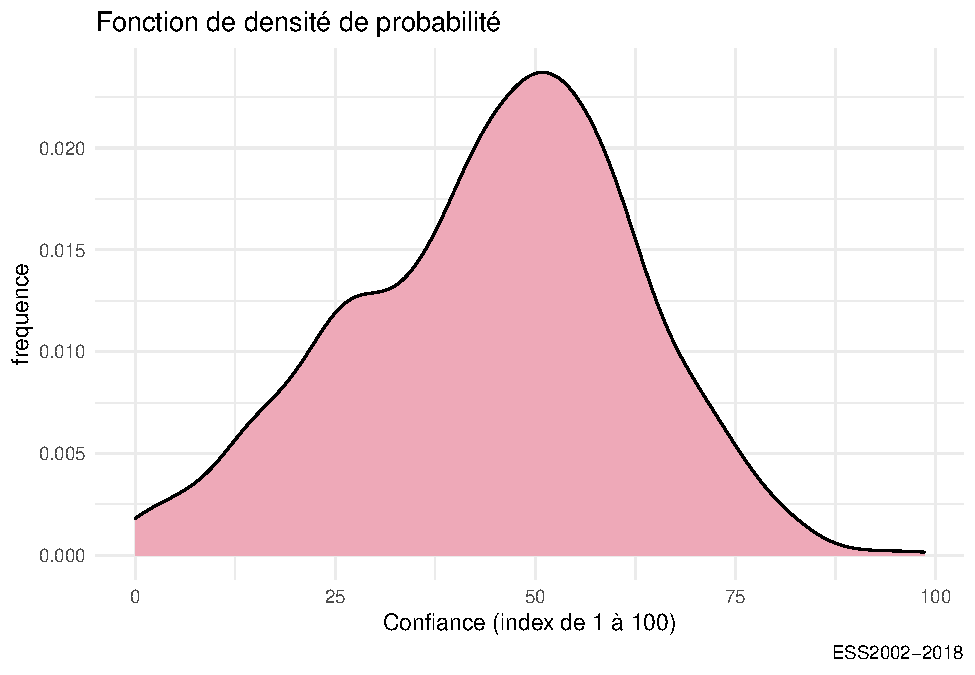
\includegraphics{bookdown-demo_files/figure-latex/304-1.pdf}

enfin on peut examiner par rapport à une distribution théorique, en l'occurrence une distribution gaussienne, ou normale, de paramètres égaux à la moyenne et la variance empirique de la distribution. L'ajustement est convenable même si on observe une déviation sur la droite. C'est pourquoi on calcule aussi la Kurtosis et le skewness de la distribution.

\begin{Shaded}
\begin{Highlighting}[]
\CommentTok{#On a déjà calculé la moyenne : mean}
\CommentTok{#il nous manque l'écart-type et }
\NormalTok{sd<-}\KeywordTok{sd}\NormalTok{(foo}\OperatorTok{$}\NormalTok{trust_institut, }\DataTypeTok{na.rm=}\OtherTok{TRUE}\NormalTok{)}
\KeywordTok{library}\NormalTok{(moments)}
\NormalTok{sk<-}\KeywordTok{skewness}\NormalTok{(foo}\OperatorTok{$}\NormalTok{trust_institut)}
\NormalTok{ks<-}\KeywordTok{kurtosis}\NormalTok{(foo}\OperatorTok{$}\NormalTok{trust_institut)}


\NormalTok{g05<-}\KeywordTok{ggplot}\NormalTok{(foo,}\KeywordTok{aes}\NormalTok{(}\DataTypeTok{x=}\NormalTok{trust_institut))}\OperatorTok{+}\StringTok{   }
\StringTok{  }\KeywordTok{labs}\NormalTok{(}\DataTypeTok{title=} \StringTok{"Distribution de la confiance institutionnelle"}\NormalTok{, }\DataTypeTok{caption=}\StringTok{"ESS2002-2018"}\NormalTok{,}\DataTypeTok{y=} \StringTok{"frequence"}\NormalTok{,}\DataTypeTok{x=}\StringTok{"confiance (index de 0 à 100)"}\NormalTok{) }\OperatorTok{+}
\StringTok{  }\KeywordTok{geom_density}\NormalTok{(}\DataTypeTok{fill=}\StringTok{"pink2"}\NormalTok{)}\OperatorTok{+}
\StringTok{  }\KeywordTok{stat_function}\NormalTok{(}\DataTypeTok{fun =}\NormalTok{ dnorm,}\DataTypeTok{color=}\StringTok{"red"}\NormalTok{,}\DataTypeTok{size=}\FloatTok{1.2}\NormalTok{, }\DataTypeTok{args =} \KeywordTok{list}\NormalTok{(}\DataTypeTok{mean =}\NormalTok{moy, }\DataTypeTok{sd=}\NormalTok{sd))}
   
\NormalTok{g05}
\end{Highlighting}
\end{Shaded}

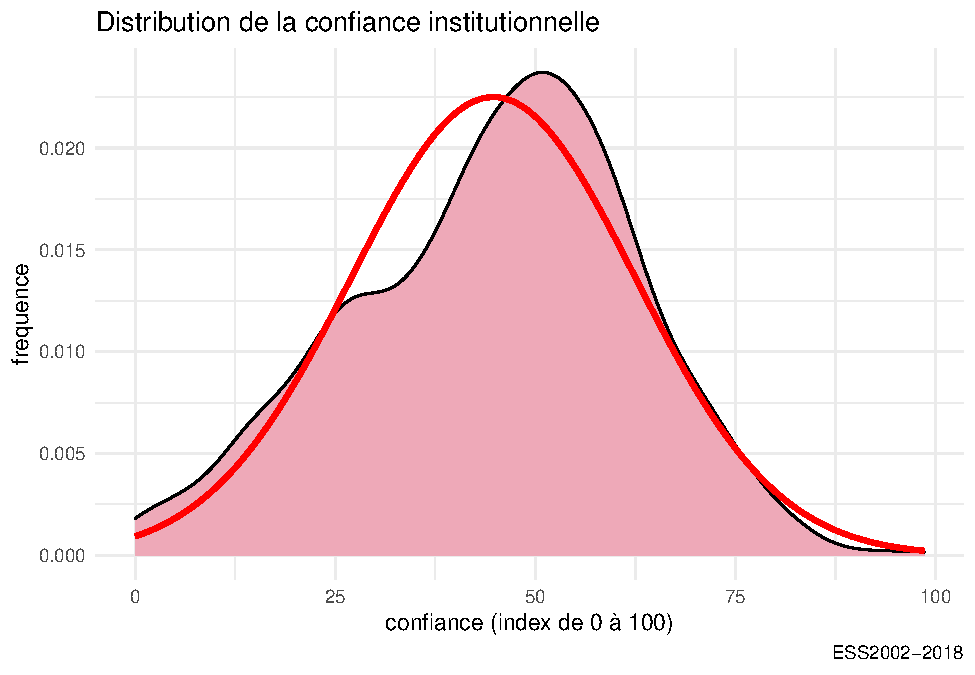
\includegraphics{bookdown-demo_files/figure-latex/305-1.pdf}

Un grand classique du test de normalité d'une distribution est le diagramme QQ

\begin{Shaded}
\begin{Highlighting}[]
\NormalTok{g06 <-}\StringTok{ }\KeywordTok{ggplot}\NormalTok{(foo, }\KeywordTok{aes}\NormalTok{(}\DataTypeTok{sample =}\NormalTok{ trust_institut)) }\OperatorTok{+}\StringTok{ }
\StringTok{  }\KeywordTok{stat_qq}\NormalTok{() }\OperatorTok{+}\StringTok{ }\KeywordTok{stat_qq_line}\NormalTok{()}\OperatorTok{+}\StringTok{ }
\StringTok{  }\KeywordTok{labs}\NormalTok{(}\DataTypeTok{title=} \StringTok{"QQplot confiance interpersonnelle"}\NormalTok{, }\DataTypeTok{caption=}\StringTok{"ESS2002-2018"}\NormalTok{,}\DataTypeTok{y=} \StringTok{"Echantillon"}\NormalTok{,}\DataTypeTok{x=}\StringTok{"Théorique"}\NormalTok{) }
\NormalTok{g06}
\end{Highlighting}
\end{Shaded}

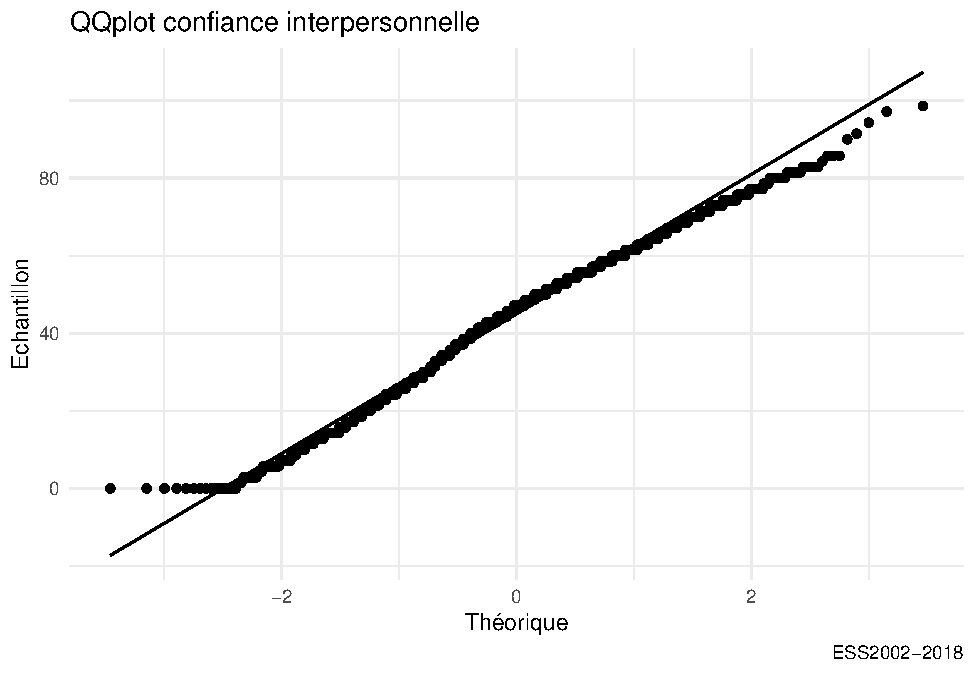
\includegraphics{bookdown-demo_files/figure-latex/306-1.pdf}

On fini cette étude détaillée par l'ajustement d'abord d'un modèle (loi normale) aux données. Ensuite d'un modèle de mélange ( Mixture model) par lequel on défiit la loi de distribution sous jascente, comme un mélange entre deux populations normale de paramètres distincts.

\url{https://tinyheero.github.io/2015/10/13/mixture-model.html}

\begin{Shaded}
\begin{Highlighting}[]
\NormalTok{df0<-df }\OperatorTok\StringTok{ }\KeywordTok{na.omit}\NormalTok{() }
\KeywordTok{library}\NormalTok{(MASS)}
\NormalTok{fit<-}\KeywordTok{fitdistr}\NormalTok{(df0}\OperatorTok{$}\NormalTok{trust_interpersonnel,}\StringTok{"normal"}\NormalTok{) }
\NormalTok{fit}
\end{Highlighting}
\end{Shaded}

\begin{verbatim}
##       mean           sd     
##   52.48548790   16.57617220 
##  ( 0.09344363) ( 0.06607462)
\end{verbatim}

\begin{Shaded}
\begin{Highlighting}[]
\NormalTok{g07<-}\StringTok{ }\NormalTok{g05}\OperatorTok{+}\KeywordTok{stat_function}\NormalTok{(}\DataTypeTok{fun =}\NormalTok{  dnorm ,}\DataTypeTok{color=}\StringTok{"orange"}\NormalTok{,}\DataTypeTok{size=}\FloatTok{1.2}\NormalTok{, }\DataTypeTok{args =} \KeywordTok{list}\NormalTok{( }\DataTypeTok{mean=}\FloatTok{52.48}\NormalTok{,  }\DataTypeTok{sd=}\FloatTok{16.57}\NormalTok{))}
\NormalTok{g07}
\end{Highlighting}
\end{Shaded}

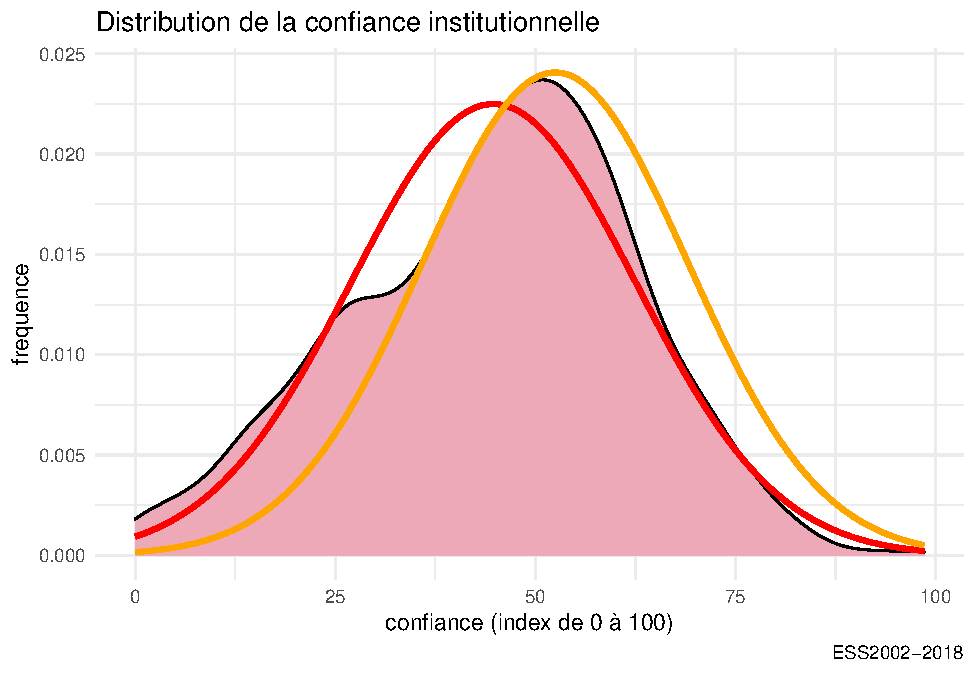
\includegraphics{bookdown-demo_files/figure-latex/307-1.pdf}

\begin{Shaded}
\begin{Highlighting}[]
\KeywordTok{library}\NormalTok{(mixtools)}
\NormalTok{trust =}\StringTok{ }\NormalTok{foo}\OperatorTok{$}\NormalTok{trust_institut}
\NormalTok{mixmdl =}\StringTok{ }\KeywordTok{normalmixEM}\NormalTok{(trust, }\DataTypeTok{k=}\DecValTok{2}\NormalTok{)}
\end{Highlighting}
\end{Shaded}

\begin{verbatim}
## number of iterations= 269
\end{verbatim}

\begin{Shaded}
\begin{Highlighting}[]
\NormalTok{mixmdl}\OperatorTok{$}\NormalTok{mu}
\end{Highlighting}
\end{Shaded}

\begin{verbatim}
## [1] 20.77247 50.86798
\end{verbatim}

\begin{Shaded}
\begin{Highlighting}[]
\NormalTok{mixmdl}\OperatorTok{$}\NormalTok{sigma}
\end{Highlighting}
\end{Shaded}

\begin{verbatim}
## [1] 10.37740 13.51802
\end{verbatim}

\begin{Shaded}
\begin{Highlighting}[]
\NormalTok{mixmdl}\OperatorTok{$}\NormalTok{lambda}
\end{Highlighting}
\end{Shaded}

\begin{verbatim}
## [1] 0.2034333 0.7965667
\end{verbatim}

\begin{Shaded}
\begin{Highlighting}[]
\KeywordTok{plot}\NormalTok{(mixmdl,}\DataTypeTok{which=}\DecValTok{2}\NormalTok{)}
\KeywordTok{lines}\NormalTok{(}\KeywordTok{density}\NormalTok{(trust), }\DataTypeTok{lty=}\DecValTok{2}\NormalTok{, }\DataTypeTok{lwd=}\DecValTok{2}\NormalTok{)}
\end{Highlighting}
\end{Shaded}

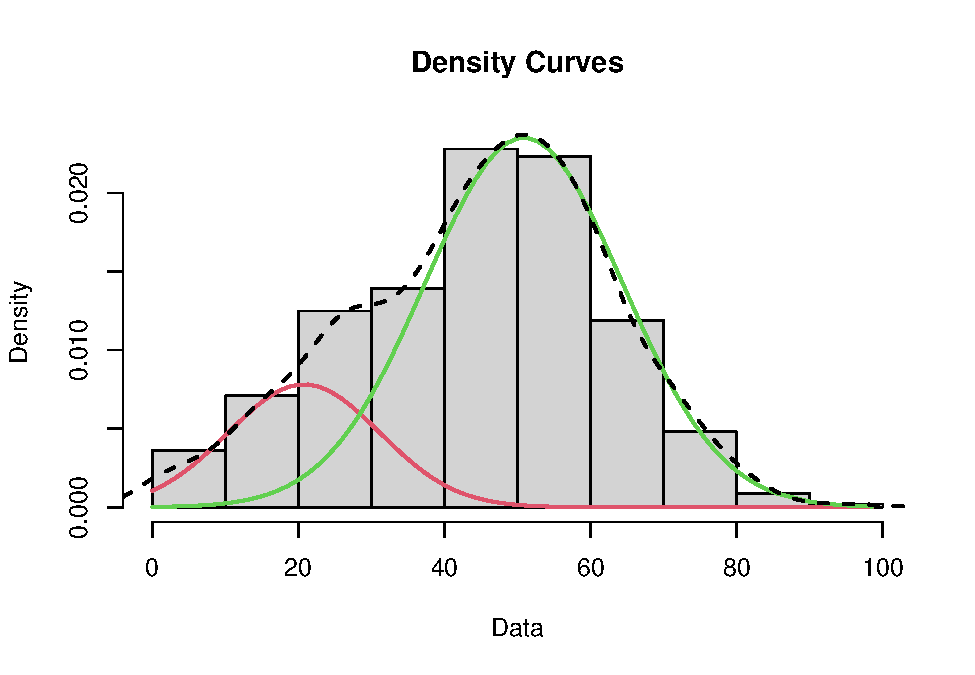
\includegraphics{bookdown-demo_files/figure-latex/307-2.pdf}

Finalement si notre distribution est univariée, car n'étudiant qu'une variable, on peut quand distinguer deux population distinctes.

\hypertarget{dautres-muxe9thodes}{%
\subsubsection{D'autres méthodes}\label{dautres-muxe9thodes}}

boxplot

violin plot

barcode

\hypertarget{quand-la-variable-est-qualitative}{%
\subsection{Quand la variable est qualitative}\label{quand-la-variable-est-qualitative}}

Quand la variable est qualitative, que ses variables sont discrètes, la manière de représenter la plus commune est le fameux camembert que les experts écartent. Un diagramme en barre représente mieux les proportions.

Un premier exemple pour représenter les vagues d'enquêtes

\begin{Shaded}
\begin{Highlighting}[]
\NormalTok{g08<-}\KeywordTok{ggplot}\NormalTok{(df,}\KeywordTok{aes}\NormalTok{(}\DataTypeTok{x=}\NormalTok{age))}\OperatorTok{+}
\StringTok{  }\KeywordTok{geom_bar}\NormalTok{(}\DataTypeTok{fill=}\StringTok{"skyblue"}\NormalTok{)}\OperatorTok{+}
\StringTok{  }\KeywordTok{labs}\NormalTok{(}\DataTypeTok{title=} \StringTok{"Evolution de la confiance interpersonnelle"}\NormalTok{, }\DataTypeTok{caption=}\StringTok{"ESS2002-2018"}\NormalTok{,}\DataTypeTok{y=} \StringTok{"frequence"}\NormalTok{,}\DataTypeTok{x=}\StringTok{"Vague d'enquête") }
\StringTok{g08}
\end{Highlighting}
\end{Shaded}

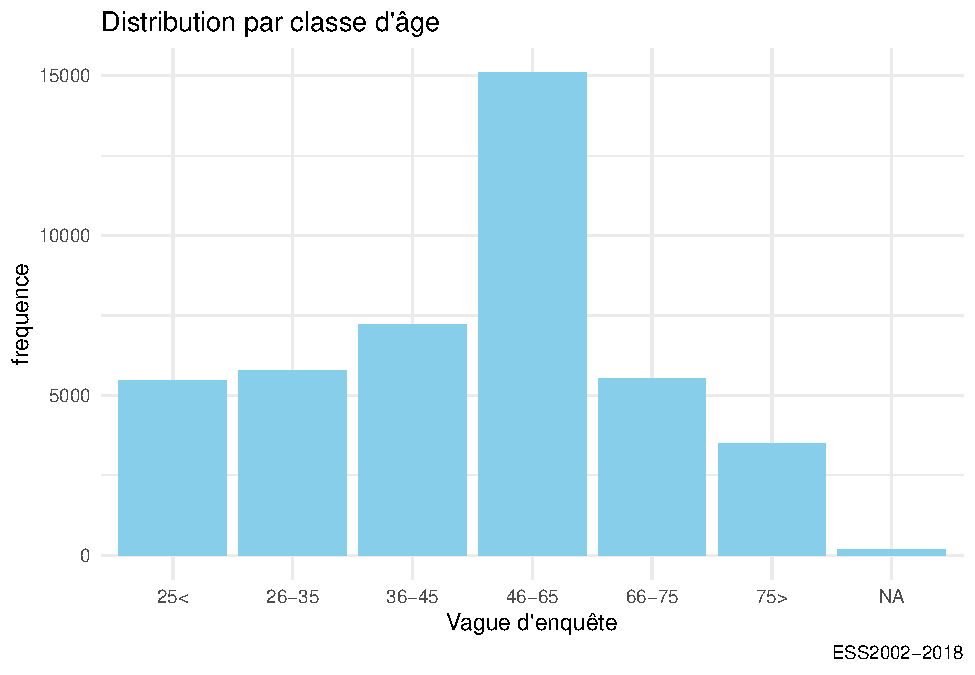
\includegraphics{bookdown-demo_files/figure-latex/308-1.pdf}

en \% et en 2 jeux de couleurs standard et couleur

\begin{Shaded}
\begin{Highlighting}[]
\NormalTok{foo<-df }\OperatorTok\KeywordTok{filter}\NormalTok{(}\OperatorTok{!}\KeywordTok{is.na}\NormalTok{(age))}
\NormalTok{g10<-}\KeywordTok{ggplot}\NormalTok{(foo,}\KeywordTok{aes}\NormalTok{(}\DataTypeTok{x=}\NormalTok{age, }\DataTypeTok{y =} \KeywordTok{prop.table}\NormalTok{(}\KeywordTok{stat}\NormalTok{(count)),}\DataTypeTok{label =}\NormalTok{ scales}\OperatorTok{::}\KeywordTok{percent}\NormalTok{(}\KeywordTok{prop.table}\NormalTok{(}\KeywordTok{stat}\NormalTok{(count)))))}\OperatorTok{+}
\StringTok{  }\KeywordTok{geom_bar}\NormalTok{(}\KeywordTok{aes}\NormalTok{(}\DataTypeTok{fill =}\NormalTok{ age)) }\OperatorTok{+}\StringTok{  }
\StringTok{  }\KeywordTok{coord_flip}\NormalTok{()}\OperatorTok{+}\StringTok{ }
\StringTok{  }\KeywordTok{labs}\NormalTok{(}\DataTypeTok{title=} \StringTok{"Répartition de la population par classe d'âge"}\NormalTok{, }\DataTypeTok{caption=}\StringTok{"ESS2002-2018"}\NormalTok{,}\DataTypeTok{y=} \StringTok{"%"}\NormalTok{,}\DataTypeTok{x=}\StringTok{"classes d'age"}\NormalTok{) }\OperatorTok{+}
\StringTok{  }\KeywordTok{scale_y_continuous}\NormalTok{(}\DataTypeTok{labels =}\NormalTok{ scales}\OperatorTok{::}\NormalTok{percent)}\OperatorTok{+}
\StringTok{  }\KeywordTok{geom_text}\NormalTok{(}\DataTypeTok{stat =} \StringTok{'count'}\NormalTok{,}\DataTypeTok{position =} \KeywordTok{position_dodge}\NormalTok{(.}\DecValTok{9}\NormalTok{),  }\DataTypeTok{hjust =} \DecValTok{1}\NormalTok{, }\DataTypeTok{size =} \DecValTok{3}\NormalTok{) }


\NormalTok{g10}
\end{Highlighting}
\end{Shaded}

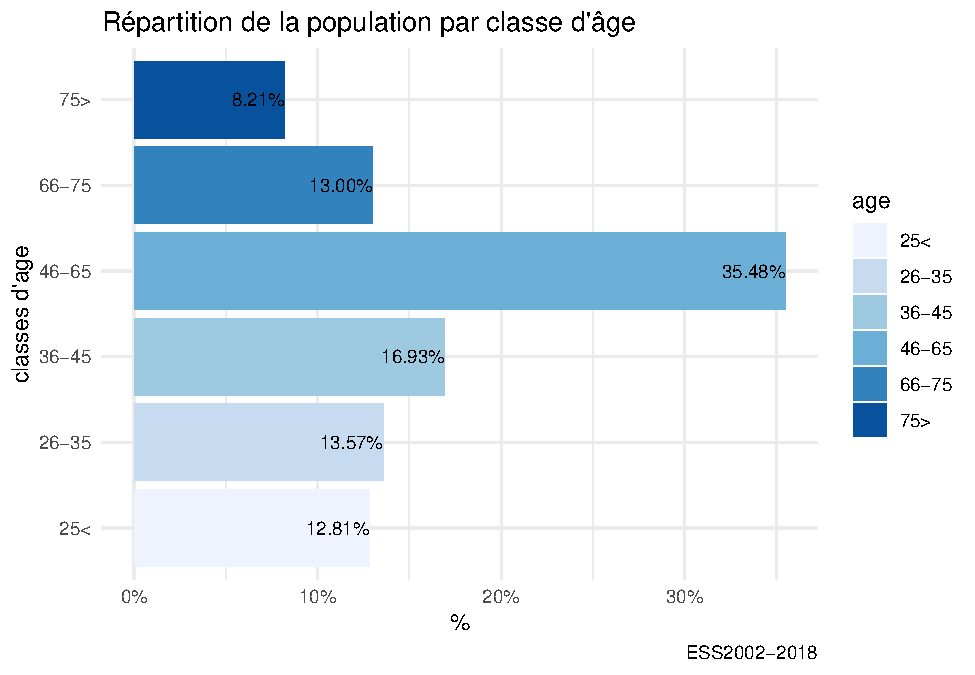
\includegraphics{bookdown-demo_files/figure-latex/309-1.pdf}

si on tient au diagramme en cercle, autant opter pour un treemap avec la bibliothèque treemapifi

\begin{Shaded}
\begin{Highlighting}[]
\NormalTok{foo<-df }\OperatorTok\KeywordTok{filter}\NormalTok{(}\OperatorTok{!}\KeywordTok{is.na}\NormalTok{(age))}
\NormalTok{g10<-}\KeywordTok{ggplot}\NormalTok{(foo,}\KeywordTok{aes}\NormalTok{(}\DataTypeTok{x=}\StringTok{""}\NormalTok{, }\DataTypeTok{y =} \KeywordTok{prop.table}\NormalTok{(}\KeywordTok{stat}\NormalTok{(count)),}\DataTypeTok{label =}\NormalTok{ scales}\OperatorTok{::}\KeywordTok{percent}\NormalTok{(}\KeywordTok{prop.table}\NormalTok{(}\KeywordTok{stat}\NormalTok{(count)))))}\OperatorTok{+}
\StringTok{  }\KeywordTok{geom_bar}\NormalTok{(}\KeywordTok{aes}\NormalTok{(}\DataTypeTok{fill =}\NormalTok{ age)) }\OperatorTok{+}\StringTok{  }
\StringTok{  }\KeywordTok{labs}\NormalTok{(}\DataTypeTok{title=} \StringTok{"Répartition de la population par classe d'âge"}\NormalTok{, }\DataTypeTok{caption=}\StringTok{"ESS2002-2018"}\NormalTok{,}\DataTypeTok{y=} \StringTok{"%"}\NormalTok{,}\DataTypeTok{x=}\StringTok{"classes d'age"}\NormalTok{) }\OperatorTok{+}
\StringTok{  }\KeywordTok{geom_text}\NormalTok{(}\DataTypeTok{stat =} \StringTok{'count'}\NormalTok{,}\DataTypeTok{position =} \KeywordTok{position_dodge}\NormalTok{(.}\DecValTok{9}\NormalTok{),  }\DataTypeTok{hjust =} \DecValTok{1}\NormalTok{, }\DataTypeTok{size =} \DecValTok{3}\NormalTok{) }\OperatorTok{+}\StringTok{ }
\StringTok{  }\KeywordTok{coord_polar}\NormalTok{(}\StringTok{"y"}\NormalTok{, }\DataTypeTok{start=}\DecValTok{0}\NormalTok{)}



\NormalTok{g10}
\end{Highlighting}
\end{Shaded}

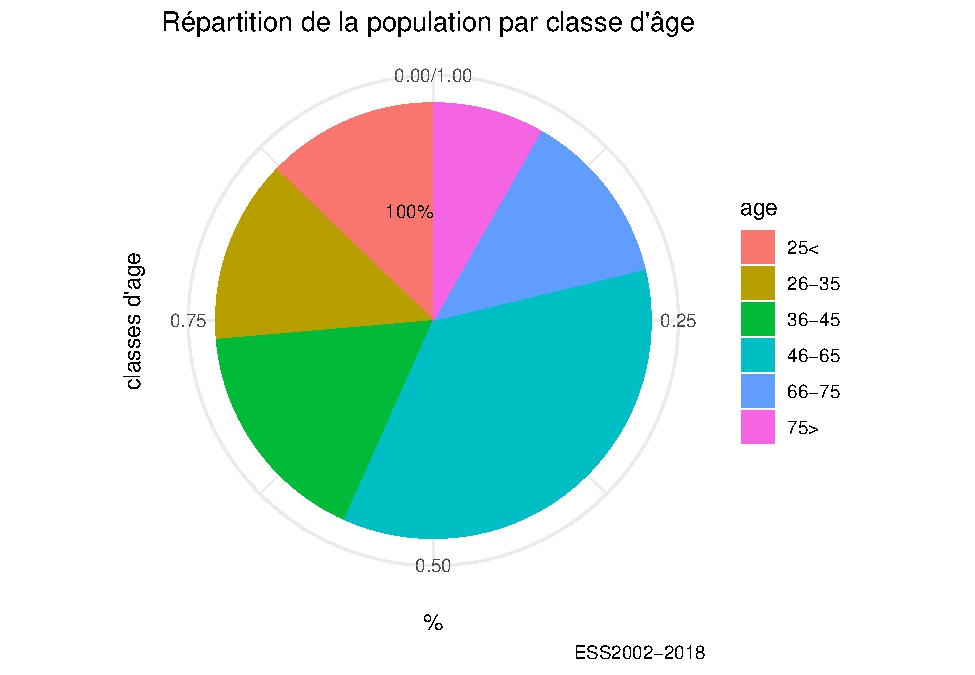
\includegraphics{bookdown-demo_files/figure-latex/310-1.pdf}
\url{https://cran.r-project.org/web/packages/treemapify/vignettes/introduction-to-treemapify.html}

si on tient au diagramme en cercle, autant opter pour un treemap avec la bibliothèque treemapifi

\begin{Shaded}
\begin{Highlighting}[]
\KeywordTok{library}\NormalTok{(treemapify)}
\NormalTok{tree1<-df }\OperatorTok\StringTok{ }
\StringTok{  }\KeywordTok{mutate}\NormalTok{(}\DataTypeTok{n=}\DecValTok{1}\NormalTok{)}\OperatorTok\KeywordTok{group_by}\NormalTok{(age) }\OperatorTok\StringTok{ }
\StringTok{  }\KeywordTok{summarize}\NormalTok{(}\DataTypeTok{n=}\KeywordTok{sum}\NormalTok{(n)) }\OperatorTok
\StringTok{  }\KeywordTok{filter}\NormalTok{(}\OperatorTok{!}\KeywordTok{is.na}\NormalTok{(age))}

\NormalTok{g11 <-}\StringTok{ }\KeywordTok{ggplot}\NormalTok{(tree1, }\KeywordTok{aes}\NormalTok{(}\DataTypeTok{area =}\NormalTok{ n, }\DataTypeTok{fill=}\NormalTok{n),}\DataTypeTok{label=}\NormalTok{age) }\OperatorTok{+}
\StringTok{  }\KeywordTok{geom_treemap}\NormalTok{() }\OperatorTok{+}\StringTok{   }\KeywordTok{geom_treemap_text}\NormalTok{(}\KeywordTok{aes}\NormalTok{(}\DataTypeTok{label=}\NormalTok{age),}\DataTypeTok{colour =} \StringTok{"white"}\NormalTok{, }\DataTypeTok{place =} \StringTok{"centre"}\NormalTok{,}\DataTypeTok{grow =} \OtherTok{TRUE}\NormalTok{)}\OperatorTok{+}
\StringTok{  }\KeywordTok{labs}\NormalTok{(}\DataTypeTok{title=} \StringTok{"Répartition de la population par classe d'âge"}\NormalTok{, }\DataTypeTok{caption=}\StringTok{"ESS2002-2018"}\NormalTok{,}\DataTypeTok{y=} \OtherTok{NULL}\NormalTok{,}\DataTypeTok{x=}\OtherTok{NULL}\NormalTok{) }

\NormalTok{g11}
\end{Highlighting}
\end{Shaded}

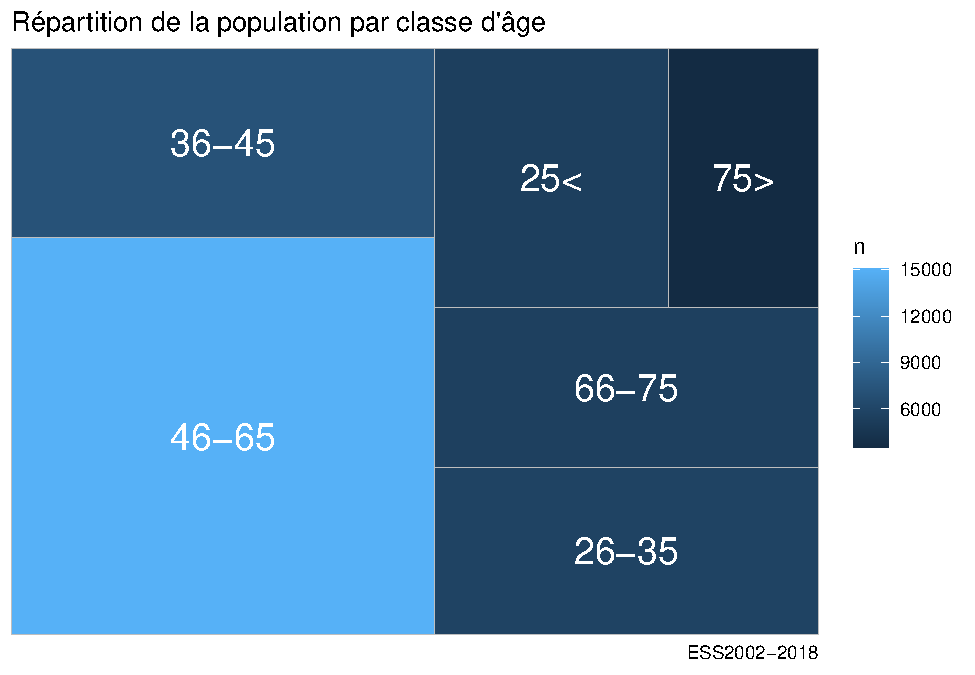
\includegraphics{bookdown-demo_files/figure-latex/311-1.pdf}

\hypertarget{analyse-bivariuxe9e}{%
\section{Analyse bivariée}\label{analyse-bivariuxe9e}}

Comme son nom l'indique, il s'agit d'examiner la relation entre deux variables et d'étudier leur distribution conjointe.

\begin{enumerate}
\def\labelenumi{\alph{enumi})}
\tightlist
\item
  deux variables quantitatives
\item
  deux variable qualitatives
\item
  une variable quanti et une variable quali.
\end{enumerate}

\hypertarget{diagrammes-xy---la-magie-des-corruxe9lations}{%
\subsection{Diagrammes xy - la magie des corrélations}\label{diagrammes-xy---la-magie-des-corruxe9lations}}

\begin{enumerate}
\def\labelenumi{\alph{enumi})}
\tightlist
\item
  par comparer des distribution de plusieurs groupes (variables catégorielles)
\item
  par comparer des moyennes d'une variable dépendante en fonction de plusieurs variables indépendantes catégorielle
\item
  mesurer l'association entre deux variables qualitatives
\end{enumerate}

venons en à analyser les relation entre deux variables quantitatives.

\begin{Shaded}
\begin{Highlighting}[]
\NormalTok{foo<-df }\OperatorTok\KeywordTok{filter}\NormalTok{(cntry}\OperatorTok{==}\StringTok{"FR"} \OperatorTok{&}\StringTok{ }\NormalTok{Year}\OperatorTok{==}\StringTok{"2018"}\NormalTok{)}

\NormalTok{g31<-}\StringTok{ }\KeywordTok{ggplot}\NormalTok{(foo, }\KeywordTok{aes}\NormalTok{(}\DataTypeTok{x=}\NormalTok{ trust_interpersonnel,}\DataTypeTok{y=}\NormalTok{trust_institut)) }\OperatorTok{+}
\StringTok{  }\KeywordTok{geom_point}\NormalTok{( }\DataTypeTok{size=}\FloatTok{0.1}\NormalTok{)}
     
\NormalTok{g31}
\end{Highlighting}
\end{Shaded}

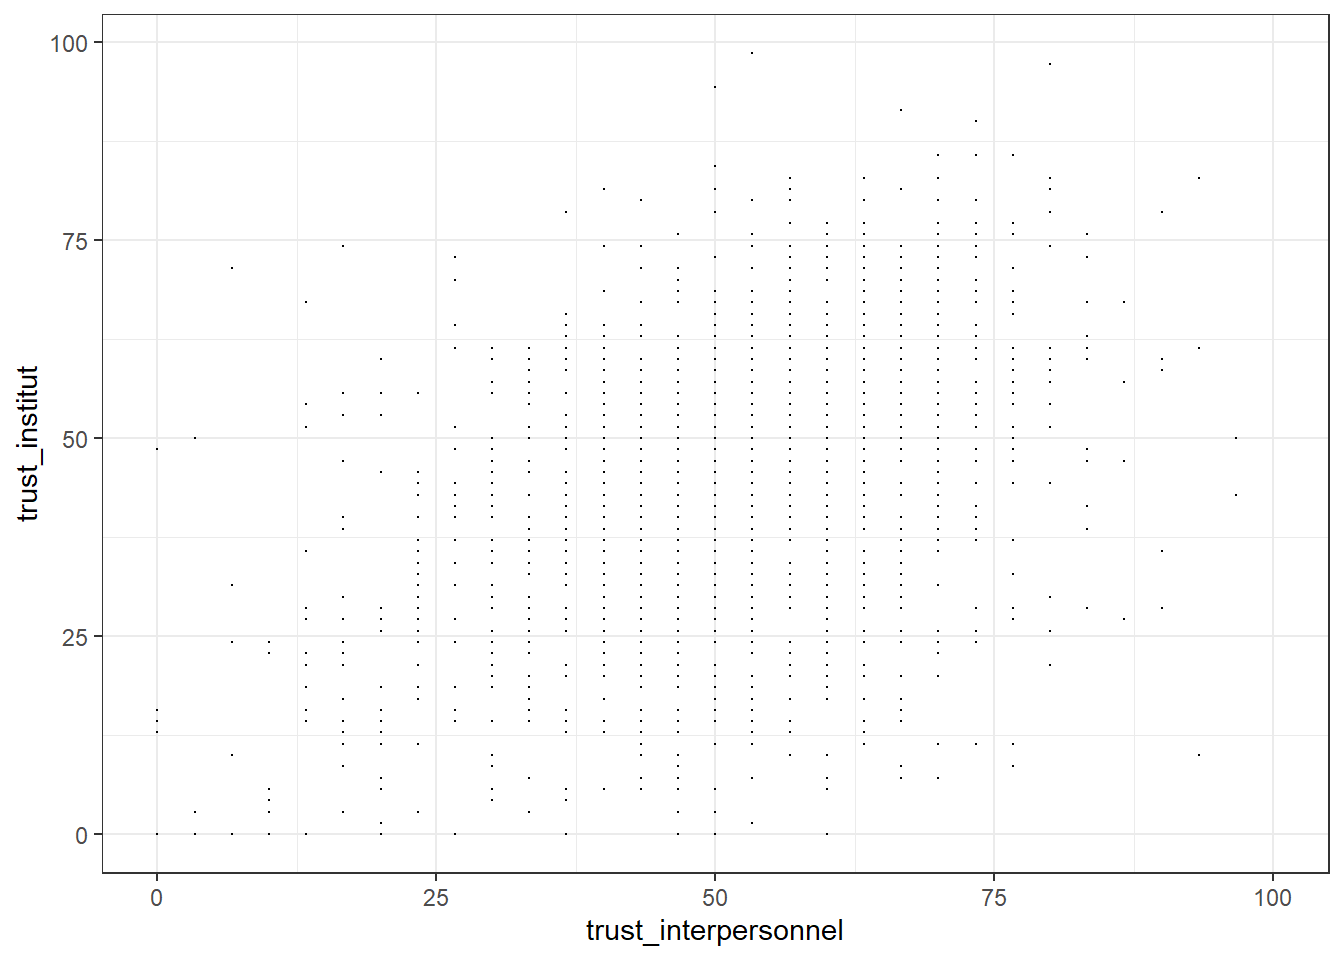
\includegraphics{bookdown-demo_files/figure-latex/312-1.pdf}
Ce graphe est peu clair, il y a trop de points qui prennent des valeurs discrètes. Une astuce est de donner une position aléatoire pour sur disperser, on fait mieux apparaitre la densité de points. On ajoute la représentation de deux courbe d'ajustement, l'une linéraire et l'autre non linéaires.

Mais en attendant en voici un calcul élémentaire.

le calcul de la variance

\[{SS}_{xx} = \sum (x - \bar{x})^2 = \sum x^2 - \frac {(\sum x)^2}{n}\]
le calcul de la covariance

\[{SS}_{xy} = \sum (x - \bar{x})(y - \bar{y}) = \sum xy - \frac {(\sum x)(\sum y)}{n}\]
et la corrélation qui est le rapport de la covariance sur la racine carrée du produit des variances de x et y.

\[r = \frac {{SS}_{xy}}{\sqrt {{SS}_{xx}{SS}_{yy}}}\]

la corrélation est de l'ordre d'un peu plus 0,42 ce qui est assez élevé mais laisse une certaine indépendance des variables. Elle désignent des objets liés mais différents.

\begin{Shaded}
\begin{Highlighting}[]
\CommentTok{#psych}
\NormalTok{r<-}\KeywordTok{cor.test}\NormalTok{(foo}\OperatorTok{$}\NormalTok{trust_interpersonnel, foo}\OperatorTok{$}\NormalTok{trust_institut)}
\NormalTok{rp<-}\KeywordTok{round}\NormalTok{(r}\OperatorTok{$}\NormalTok{estimate,}\DecValTok{3}\NormalTok{)}
\NormalTok{rp}
\end{Highlighting}
\end{Shaded}

\begin{verbatim}
##   cor 
## 0.404
\end{verbatim}

Amélirons de grapf

\begin{Shaded}
\begin{Highlighting}[]
\KeywordTok{library}\NormalTok{(ggExtra)}
\NormalTok{g32<-}\KeywordTok{ggplot}\NormalTok{(foo, }\KeywordTok{aes}\NormalTok{(}\DataTypeTok{x=}\NormalTok{ trust_interpersonnel,}\DataTypeTok{y=}\NormalTok{trust_institut)) }\OperatorTok{+}
\StringTok{  }\KeywordTok{geom_point}\NormalTok{(}\DataTypeTok{position =} \StringTok{"jitter"}\NormalTok{, }\DataTypeTok{size=}\FloatTok{0.1}\NormalTok{, }\DataTypeTok{color=}\StringTok{"grey"}\NormalTok{)}\OperatorTok{+}
\StringTok{  }\KeywordTok{geom_smooth}\NormalTok{(}\DataTypeTok{method=}\StringTok{"lm"}\NormalTok{, }\DataTypeTok{se=}\OtherTok{TRUE}\NormalTok{) }\OperatorTok{+}
\StringTok{  }\KeywordTok{geom_smooth}\NormalTok{(}\DataTypeTok{method=}\StringTok{"gam"}\NormalTok{,}\DataTypeTok{color=}\StringTok{"red"}\NormalTok{)     }\OperatorTok{+}
\StringTok{  }\KeywordTok{labs}\NormalTok{(}\DataTypeTok{title =} \StringTok{"Relation entre confiance }\CharTok{\textbackslash{}n}\StringTok{institutionnelle et interpersonnelle"}\NormalTok{, }
       \DataTypeTok{subtitle =} \KeywordTok{paste}\NormalTok{(}\StringTok{"r de pearson: "}\NormalTok{,rp ),}
       \DataTypeTok{x=} \StringTok{"Confiance interpersonnelle"}\NormalTok{,}
       \DataTypeTok{y=}\StringTok{" Confiance institutionnelle"}\NormalTok{)}

\KeywordTok{ggMarginal}\NormalTok{(g32  ,}\DataTypeTok{type =} \StringTok{"density"}\NormalTok{, }\DataTypeTok{fill =} \StringTok{"Royalblue1"}\NormalTok{, }\DataTypeTok{alpha=}\NormalTok{.}\DecValTok{5}\NormalTok{)}
\end{Highlighting}
\end{Shaded}

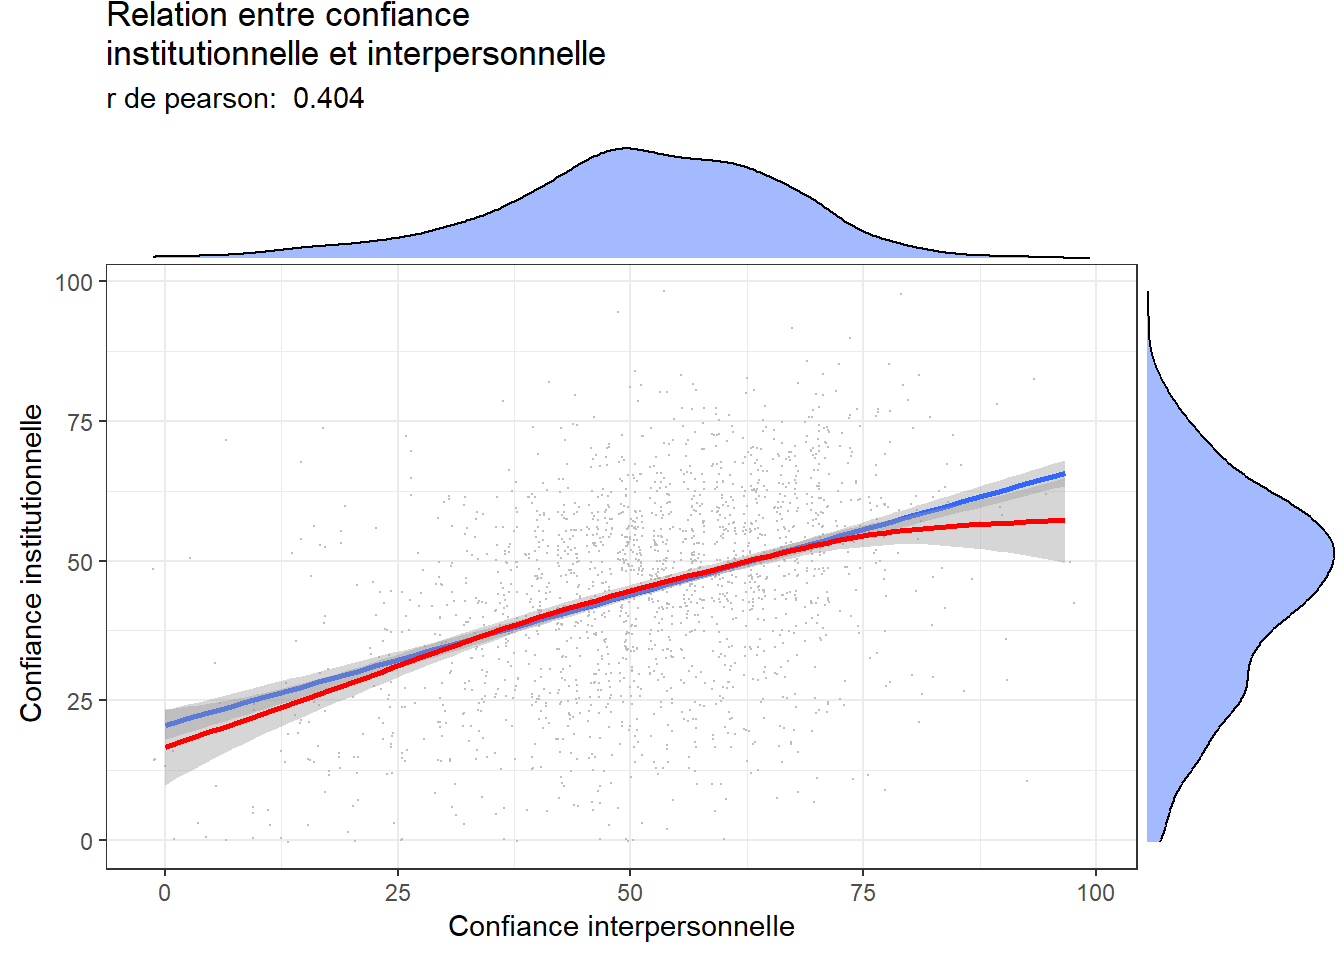
\includegraphics{bookdown-demo_files/figure-latex/315-1.pdf}

on peut souhaiter ajouter une droite des moindre carrés (calculée pour chaque vague d'enquête pour évaluer la stabilité de la relation dans le temps). Les lignes sont parallèles, la corrélation ne change pas dans le temps, c'est une relation stable. Les deux formes de confiance vont dans le meme sens. On verra dans un autre chapitre comment calculer ces droites de corrélations.

Une autre représentation plus éclatée qui ne montre rien de plus que la régularité

Une autre façon de représenter est celle de carte de densité de probabilité.

\begin{Shaded}
\begin{Highlighting}[]
\NormalTok{g32<-}\KeywordTok{ggplot}\NormalTok{(foo, }\KeywordTok{aes}\NormalTok{(}\DataTypeTok{x=}\NormalTok{ trust_interpersonnel,}\DataTypeTok{y=}\NormalTok{trust_institut)) }\OperatorTok{+}
\StringTok{  }\KeywordTok{geom_point}\NormalTok{(}\DataTypeTok{position =} \StringTok{"jitter"}\NormalTok{, }\DataTypeTok{size=}\FloatTok{0.1}\NormalTok{, }\DataTypeTok{color=}\StringTok{"grey"}\NormalTok{)}\OperatorTok{+}\KeywordTok{geom_density2d}\NormalTok{()}\OperatorTok{+}
\StringTok{  }\KeywordTok{labs}\NormalTok{(}\DataTypeTok{title =} \StringTok{"Relation entre confiance institutionnelle et interpersonnelles"}\NormalTok{, }\DataTypeTok{subtitle =} \KeywordTok{paste}\NormalTok{(}\StringTok{"r de pearson: "}\NormalTok{,rp ))}
  
\NormalTok{g33<-}\KeywordTok{ggplot}\NormalTok{(foo, }\KeywordTok{aes}\NormalTok{(}\DataTypeTok{x=}\NormalTok{ trust_interpersonnel,}\DataTypeTok{y=}\NormalTok{trust_institut)) }\OperatorTok{+}
\StringTok{  }\KeywordTok{geom_density2d_filled}\NormalTok{(}\KeywordTok{aes}\NormalTok{(}\DataTypeTok{fill =}\NormalTok{ ..level.., }\DataTypeTok{color =}\NormalTok{ ..level..),}
    \DataTypeTok{contour_var =} \StringTok{"density"}\NormalTok{)}\OperatorTok{+}
\StringTok{  }\KeywordTok{labs}\NormalTok{(}\DataTypeTok{title =} \StringTok{"Relation entre confiance institutionnelle et interpersonnelles"}\NormalTok{, }\DataTypeTok{subtitle =} \KeywordTok{paste}\NormalTok{(}\StringTok{"r de pearson: "}\NormalTok{,rp ))}\OperatorTok{+}\KeywordTok{theme}\NormalTok{(}\DataTypeTok{legend.position =} \StringTok{"none"}\NormalTok{)}
  

\KeywordTok{plot_grid}\NormalTok{(g32, g33, }\DataTypeTok{labels =} \KeywordTok{c}\NormalTok{(}\StringTok{'A'}\NormalTok{, }\StringTok{'B'}\NormalTok{), }\DataTypeTok{label_size =} \DecValTok{12}\NormalTok{)}
\end{Highlighting}
\end{Shaded}

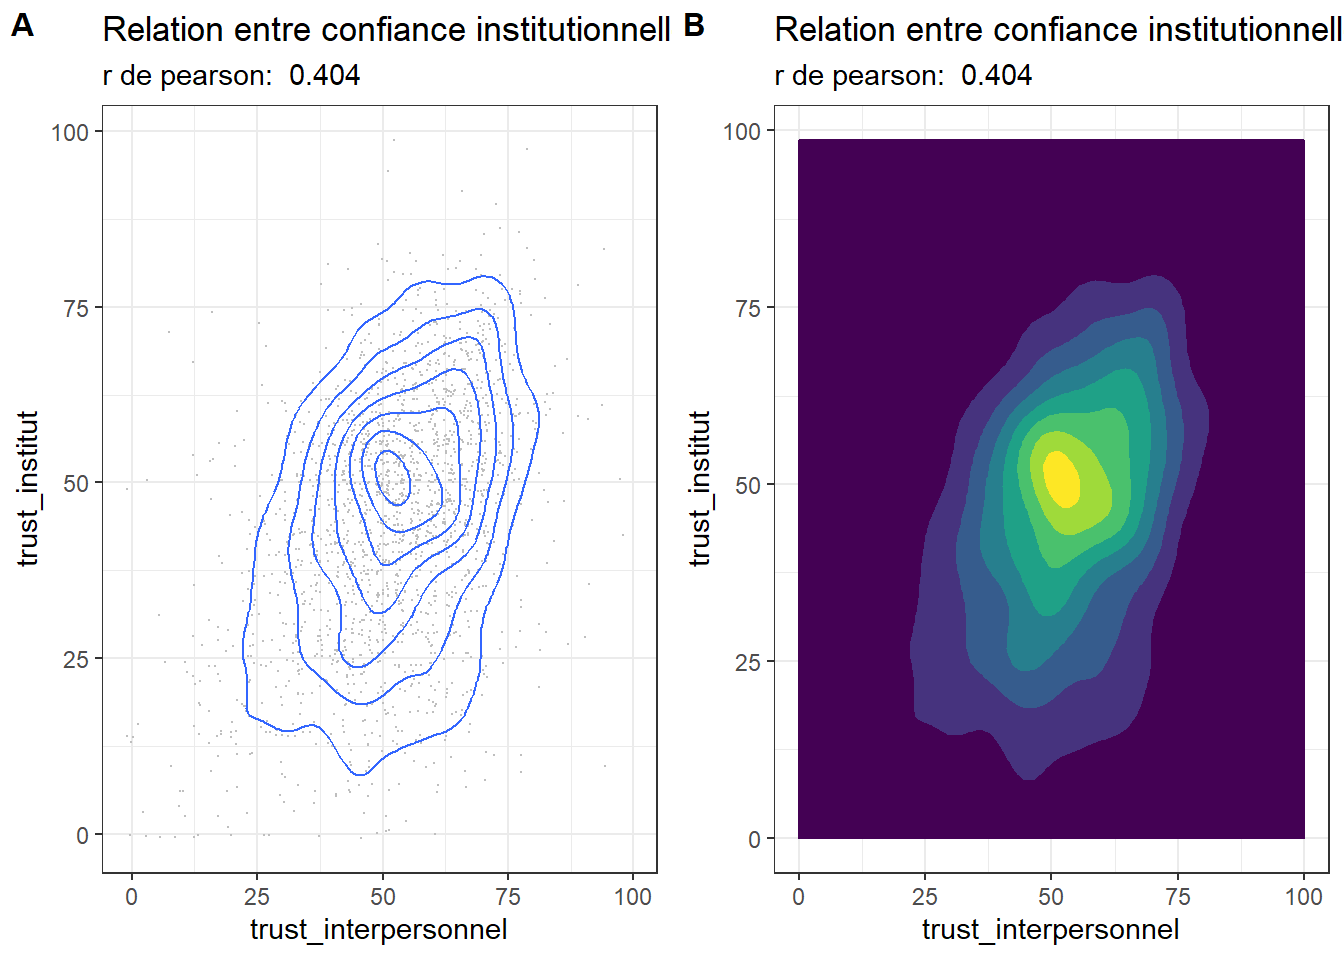
\includegraphics{bookdown-demo_files/figure-latex/316-1.pdf}

\hypertarget{comparer-les-distributions}{%
\subsection{Comparer les distributions}\label{comparer-les-distributions}}

Dans notre base on a melangé les données de l'Allemagne et de la France. On va comparer leur distribution. Et tant qu'à faire, puisque qu'on a deux variables, on va faire deux comparaions.

A cette fin, nous construisons un tableau de donnée spécifique.

\begin{Shaded}
\begin{Highlighting}[]
\CommentTok{#on recode en facteur la variable}

\NormalTok{foo <-}\StringTok{ }\NormalTok{df }\OperatorTok\StringTok{ }
\StringTok{  }\NormalTok{dplyr}\OperatorTok{::}\KeywordTok{select}\NormalTok{(cntry,trust_institut, Year,trust_interpersonnel) }\OperatorTok
\StringTok{  }\KeywordTok{filter}\NormalTok{( Year}\OperatorTok{==}\StringTok{"2018"}\NormalTok{) }\OperatorTok\StringTok{ }
\StringTok{ }\NormalTok{dplyr}\OperatorTok{::}\KeywordTok{select}\NormalTok{(}\OperatorTok{-}\NormalTok{Year)}\OperatorTok
\StringTok{ }\KeywordTok{drop_na}\NormalTok{() }\OperatorTok
\StringTok{  }\KeywordTok{gather}\NormalTok{(variable, value, }\OperatorTok{-}\NormalTok{cntry)}


\CommentTok{#on peut utiliser "facet"}
\NormalTok{g20<-}\KeywordTok{ggplot}\NormalTok{(foo,}\KeywordTok{aes}\NormalTok{(}\DataTypeTok{x=}\NormalTok{value))}\OperatorTok{+}\StringTok{ }\KeywordTok{geom_density}\NormalTok{(}\DataTypeTok{binwidth=}\DecValTok{10}\NormalTok{, }\DataTypeTok{fill=}\StringTok{"pink"}\NormalTok{)}\OperatorTok{+}\StringTok{ }\KeywordTok{facet_grid}\NormalTok{(cntry}\OperatorTok{~}\NormalTok{variable)}\OperatorTok{+}\StringTok{   }
\StringTok{  }\KeywordTok{labs}\NormalTok{(}\DataTypeTok{title=} \StringTok{"Confiance institutionnnelle"}\NormalTok{, }\DataTypeTok{caption=}\StringTok{"ESS2002-2018"}\NormalTok{,}\DataTypeTok{y=} \StringTok{"frequence"}\NormalTok{,}\DataTypeTok{x=}\StringTok{"Confiance"}\NormalTok{)}
\NormalTok{g20}
\end{Highlighting}
\end{Shaded}

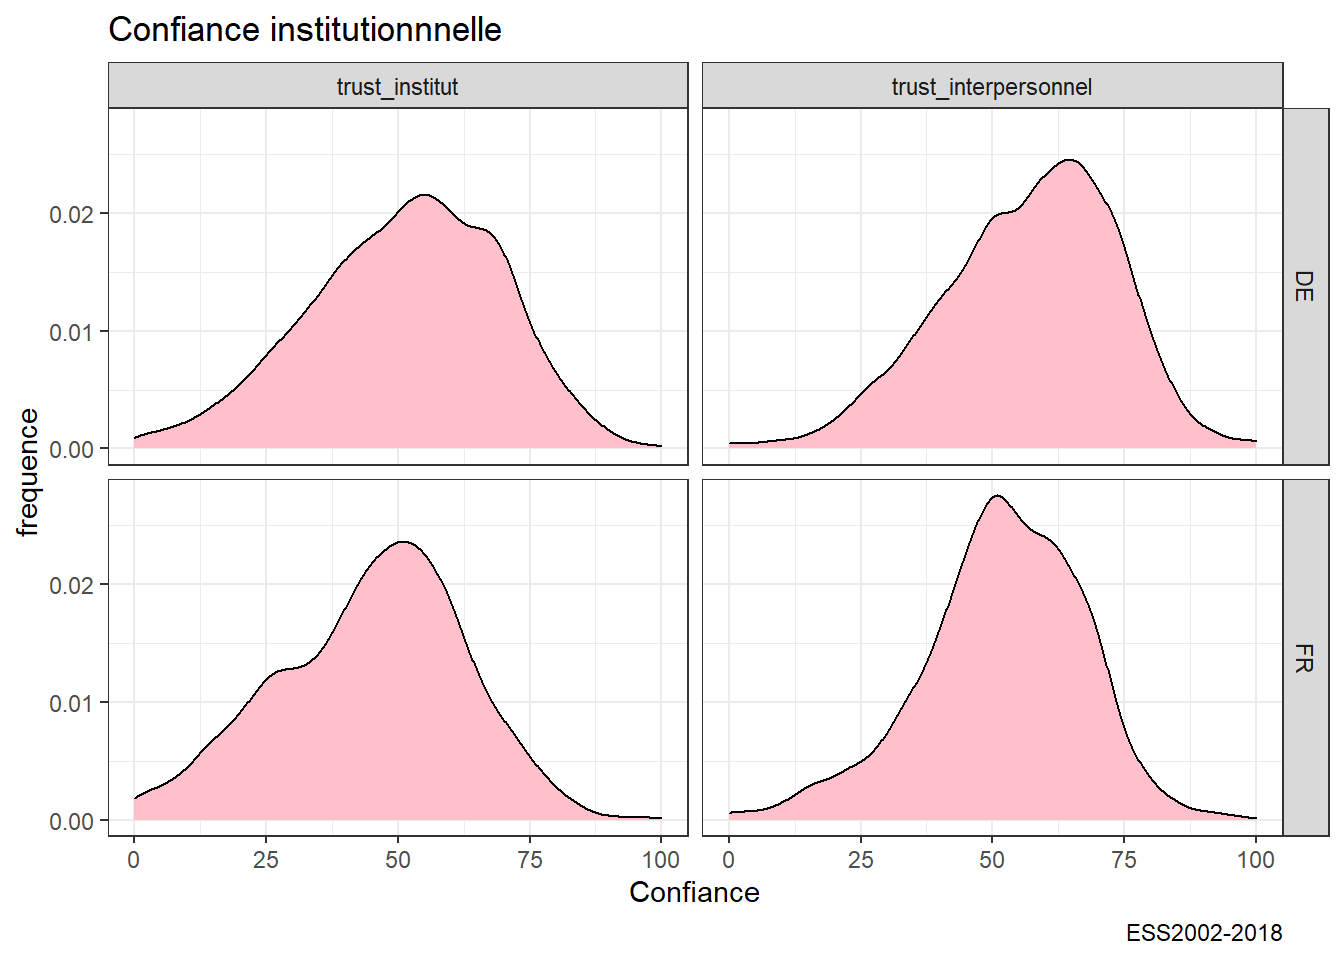
\includegraphics{bookdown-demo_files/figure-latex/317-1.pdf}

\begin{Shaded}
\begin{Highlighting}[]
\NormalTok{g21<-}\KeywordTok{ggplot}\NormalTok{(foo,}\KeywordTok{aes}\NormalTok{(}\DataTypeTok{x=}\NormalTok{variable, }\DataTypeTok{y=}\NormalTok{value))}\OperatorTok{+}\StringTok{ }\KeywordTok{geom_violin}\NormalTok{( }\DataTypeTok{fill=}\StringTok{"pink"}\NormalTok{) }\OperatorTok{+}\StringTok{ }\KeywordTok{geom_boxplot}\NormalTok{(}\DataTypeTok{width=}\FloatTok{0.1}\NormalTok{)}\OperatorTok{+}
\StringTok{  }\KeywordTok{facet_grid}\NormalTok{(cntry}\OperatorTok{~}\NormalTok{.)}\OperatorTok{+}\StringTok{   }
\StringTok{  }\KeywordTok{labs}\NormalTok{(}\DataTypeTok{title=} \StringTok{"Confiance institutionnnelle"}\NormalTok{, }\DataTypeTok{caption=}\StringTok{"ESS2002-2018"}\NormalTok{,}\DataTypeTok{y=} \StringTok{"frequence"}\NormalTok{,}\DataTypeTok{x=}\StringTok{"Confiance"}\NormalTok{)}
\NormalTok{g21}
\end{Highlighting}
\end{Shaded}

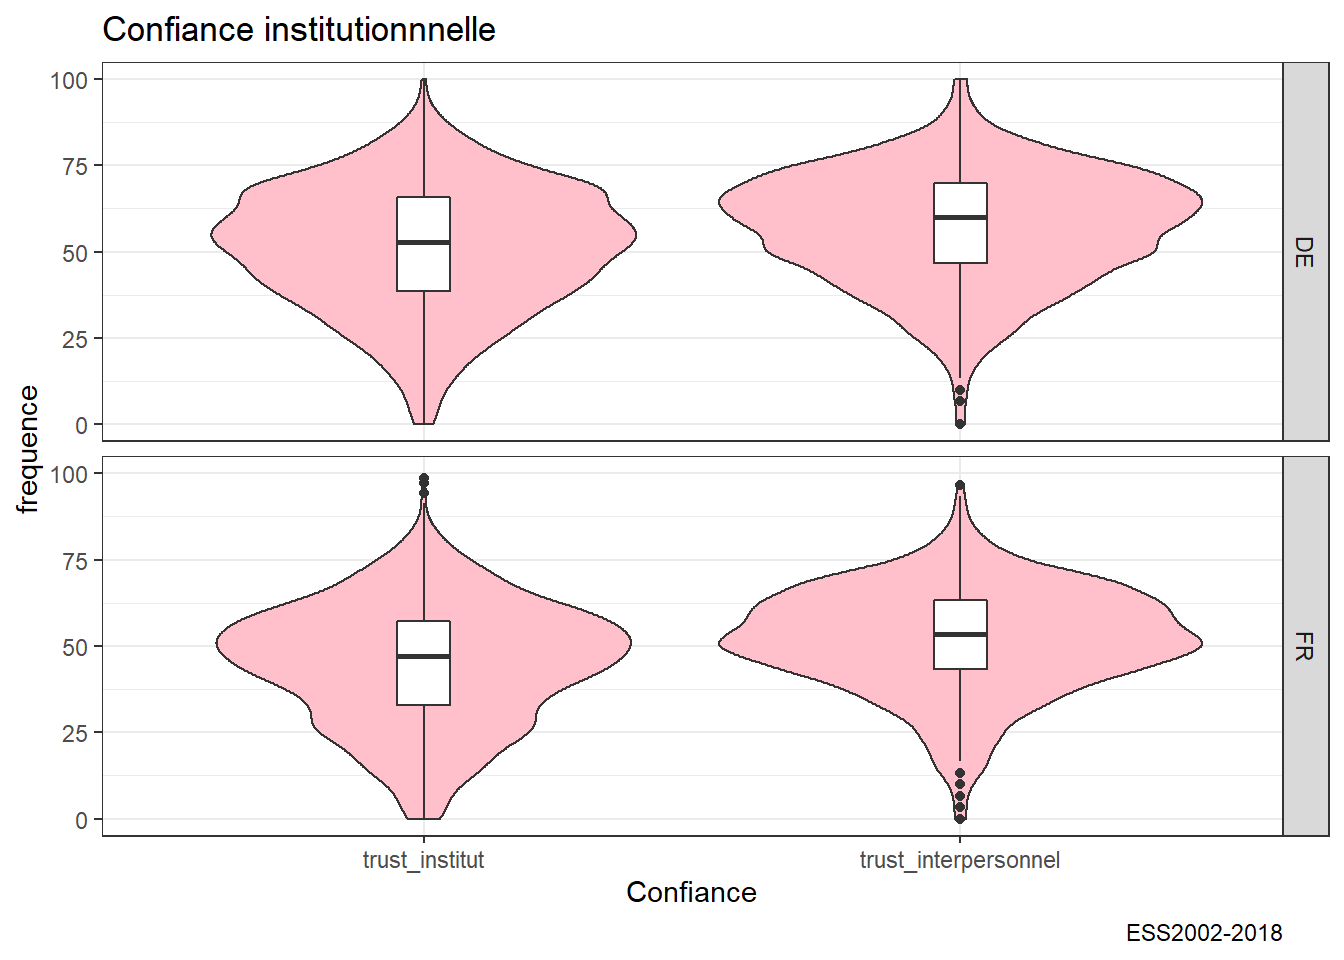
\includegraphics{bookdown-demo_files/figure-latex/317-2.pdf}

\hypertarget{comparaison-de-moyennes}{%
\subsection{Comparaison de moyennes}\label{comparaison-de-moyennes}}

ggplot traite les données qu'on lui donne. Avec les historgram on accède directement aux données. Si on souhaite représenter les moyennes et les comparer il faut une étape supplémentaire qui vise à calculer ce tableau de données : les valeurs de chacune des vague d'enquête.

\begin{Shaded}
\begin{Highlighting}[]
\NormalTok{df_wave<-df }\OperatorTok\StringTok{ }\KeywordTok{filter}\NormalTok{(cntry}\OperatorTok{==}\StringTok{"FR"} \OperatorTok{&}\StringTok{ }\NormalTok{Year}\OperatorTok{==}\StringTok{"2018"}\NormalTok{) }\OperatorTok
\StringTok{  }\KeywordTok{group_by}\NormalTok{(revenu) }\OperatorTok\StringTok{ }
\StringTok{  }\KeywordTok{summarise}\NormalTok{(}\DataTypeTok{trust_interpersonnel=}\KeywordTok{mean}\NormalTok{(trust_interpersonnel, }\DataTypeTok{na.rm=}\OtherTok{TRUE}\NormalTok{),}
            \DataTypeTok{trust_institut =}\KeywordTok{mean}\NormalTok{(trust_institut, }\DataTypeTok{na.rm=}\OtherTok{TRUE}\NormalTok{)) }\OperatorTok
\StringTok{  }\KeywordTok{filter}\NormalTok{(}\OperatorTok{!}\KeywordTok{is.na}\NormalTok{(revenu)) }\OperatorTok\StringTok{ }\KeywordTok{gather}\NormalTok{(variable, value, }\OperatorTok{-}\NormalTok{revenu)}
\NormalTok{df_wave}
\end{Highlighting}
\end{Shaded}

\begin{verbatim}
## # A tibble: 8 x 3
##   revenu                        variable             value
##   <fct>                         <chr>                <dbl>
## 1 Vie confortable               trust_interpersonnel  55.6
## 2 Se débrouille avec son revenu trust_interpersonnel  51.7
## 3 Revenu insuffisant            trust_interpersonnel  46.7
## 4 Revenu très insuffisant       trust_interpersonnel  41.4
## 5 Vie confortable               trust_institut        50.2
## 6 Se débrouille avec son revenu trust_institut        44.1
## 7 Revenu insuffisant            trust_institut        39.1
## 8 Revenu très insuffisant       trust_institut        34.5
\end{verbatim}

\begin{Shaded}
\begin{Highlighting}[]
\NormalTok{g06a<-}\KeywordTok{ggplot}\NormalTok{(df_wave,}\KeywordTok{aes}\NormalTok{(}\DataTypeTok{x=}\NormalTok{revenu,}\DataTypeTok{y=}\NormalTok{value, }\DataTypeTok{group=}\NormalTok{variable))}\OperatorTok{+}
\StringTok{  }\KeywordTok{geom_bar}\NormalTok{(}\DataTypeTok{stat=}\StringTok{"identity"}\NormalTok{,}\KeywordTok{aes}\NormalTok{(}\DataTypeTok{fill=}\NormalTok{variable), }\DataTypeTok{position =}\KeywordTok{position_dodge}\NormalTok{())}\OperatorTok{+}\StringTok{  }
\StringTok{  }\KeywordTok{labs}\NormalTok{(}\DataTypeTok{title=} \StringTok{"Confiance institutionnnelle"}\NormalTok{, }\DataTypeTok{caption=}\StringTok{"ESS2002-2018"}\NormalTok{,}\DataTypeTok{y=} \StringTok{"frequence"}\NormalTok{,}\DataTypeTok{x=}\StringTok{"Confiance"}\NormalTok{)}

\NormalTok{g06a}
\end{Highlighting}
\end{Shaded}

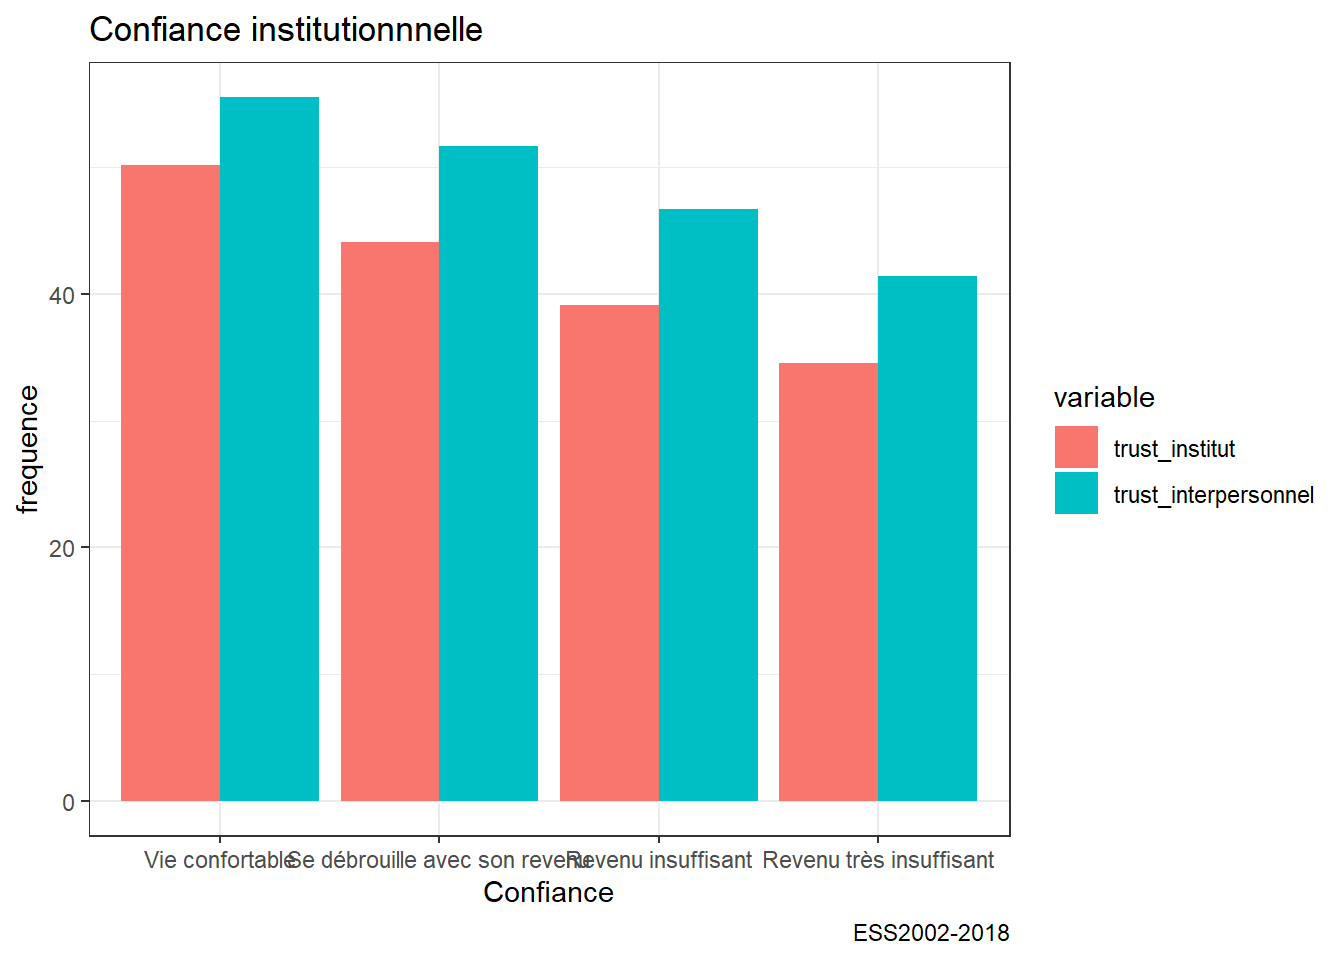
\includegraphics{bookdown-demo_files/figure-latex/318-1.pdf}

On a une solution mais pas la meilleure, on perd l'idée de variance et ce serait bien d'ajouter des barres d'intervalle de confiances , un diagramme en lignes serait plus élégant. On en profite pour corriger l'aspect des labels peu lisibles en les inclinants, et à choisir une échelle qui omettent les valeur supérieur à 70 et inférieure à 30 pour donner une vision plus respectueuses de la totalité de l'échelle qui va de 0 à 100.

Au passage on emploie à nouveau cowplot pour combiner les graphes, et ici plus précisément partager la légende des deux graphiques.

On observera que si le niveau de confiance diminue avec le revenu, la confiance interpersonnelle est plus forte, et de manière parallèle, à la confiance institutionnelle. On remarquera enfin que c'est pour les revenu les plus faibles que l'estimation est la plus imprécise ou la variance la plus grande.

\begin{Shaded}
\begin{Highlighting}[]
\NormalTok{df_wave2<-df }\OperatorTok\StringTok{ }
\StringTok{  }\KeywordTok{filter}\NormalTok{(cntry}\OperatorTok{==}\StringTok{"FR"} \OperatorTok{&}\StringTok{ }\NormalTok{Year}\OperatorTok{==}\StringTok{"2018"}\NormalTok{)}\OperatorTok
\StringTok{  }\KeywordTok{group_by}\NormalTok{(revenu) }\OperatorTok\StringTok{ }
\StringTok{  }\KeywordTok{mutate}\NormalTok{(}\DataTypeTok{n=}\DecValTok{1}\NormalTok{) }\OperatorTok
\StringTok{  }\KeywordTok{summarise}\NormalTok{(}\DataTypeTok{trust_interpersonnel_se=}\KeywordTok{sd}\NormalTok{(trust_interpersonnel, }\DataTypeTok{na.rm=}\OtherTok{TRUE}\NormalTok{), }\CommentTok{#on calcule l'écartype des deux variables}
            \DataTypeTok{trust_institut_se =}\KeywordTok{sd}\NormalTok{(trust_institut, }\DataTypeTok{na.rm=}\OtherTok{TRUE}\NormalTok{),}
            \DataTypeTok{n=}\KeywordTok{sum}\NormalTok{(n),}
            \DataTypeTok{trust_interpersonnel_se=} \DecValTok{2}\OperatorTok{*}\NormalTok{trust_interpersonnel_se}\OperatorTok{/}\KeywordTok{sqrt}\NormalTok{(n), }\CommentTok{# on calcule l'erreur type d'échantillonnage}
            \DataTypeTok{trust_institut_se=}\DecValTok{2}\OperatorTok{*}\NormalTok{trust_institut_se}\OperatorTok{/}\KeywordTok{sqrt}\NormalTok{(n)}
\NormalTok{            ) }\OperatorTok\StringTok{ }\NormalTok{dplyr}\OperatorTok{::}\KeywordTok{select}\NormalTok{(}\OperatorTok{-}\NormalTok{n) }\OperatorTok
\StringTok{  }\KeywordTok{filter}\NormalTok{(}\OperatorTok{!}\KeywordTok{is.na}\NormalTok{(revenu)) }\OperatorTok\StringTok{ }
\StringTok{  }\KeywordTok{gather}\NormalTok{(variable, value, }\OperatorTok{-}\NormalTok{revenu) }\OperatorTok\StringTok{ }\CommentTok{#on passe en format long}
\StringTok{  }\NormalTok{dplyr}\OperatorTok{::}\KeywordTok{select}\NormalTok{(}\OperatorTok{-}\NormalTok{revenu,}\OperatorTok{-}\NormalTok{variable)}\OperatorTok
\StringTok{  }\KeywordTok{rename}\NormalTok{(}\DataTypeTok{se=}\NormalTok{value)}
  
\NormalTok{df_wave3<-}\KeywordTok{cbind}\NormalTok{(df_wave,df_wave2) }\CommentTok{#on concatène les moyennes et les erreurs types}

\CommentTok{#on peut enfin produire le graphique}

\NormalTok{g06a<-}\KeywordTok{ggplot}\NormalTok{(df_wave3,}\KeywordTok{aes}\NormalTok{(}\DataTypeTok{x=}\NormalTok{revenu,}\DataTypeTok{y=}\NormalTok{value, }\DataTypeTok{group=}\NormalTok{variable))}\OperatorTok{+}
\StringTok{  }\KeywordTok{geom_line}\NormalTok{(}\DataTypeTok{stat=}\StringTok{"identity"}\NormalTok{,}\KeywordTok{aes}\NormalTok{(}\DataTypeTok{color=}\NormalTok{variable), }\DataTypeTok{size=}\FloatTok{1.5}\NormalTok{)}\OperatorTok{+}\StringTok{ }
\StringTok{  }\KeywordTok{geom_errorbar}\NormalTok{(}\KeywordTok{aes}\NormalTok{(}\DataTypeTok{ymin=}\NormalTok{value}\OperatorTok{-}\NormalTok{se, }\DataTypeTok{ymax=}\NormalTok{value}\OperatorTok{+}\NormalTok{se, }\DataTypeTok{color=}\NormalTok{variable), }\DataTypeTok{width=}\NormalTok{.}\DecValTok{2}\NormalTok{,}\DataTypeTok{position=}\KeywordTok{position_dodge}\NormalTok{(}\DecValTok{0}\NormalTok{))}\OperatorTok{+}
\StringTok{  }\KeywordTok{labs}\NormalTok{(}\DataTypeTok{title=} \StringTok{"Confiance et revenu"}\NormalTok{,}\DataTypeTok{y=} \StringTok{"Moyenne"}\NormalTok{,}\DataTypeTok{x=}\OtherTok{NULL}\NormalTok{)}\OperatorTok{+}
\StringTok{  }\KeywordTok{theme}\NormalTok{(}\DataTypeTok{axis.text.x =} \KeywordTok{element_text}\NormalTok{( }\DataTypeTok{angle=}\DecValTok{45}\NormalTok{, }\DataTypeTok{hjust =}\DecValTok{1}\NormalTok{)) }\CommentTok{#on controle l'angle et la position horizontale du label}

  
\NormalTok{g06b<-}\KeywordTok{ggplot}\NormalTok{(df_wave3,}\KeywordTok{aes}\NormalTok{(}\DataTypeTok{x=}\NormalTok{revenu,}\DataTypeTok{y=}\NormalTok{value, }\DataTypeTok{group=}\NormalTok{variable))}\OperatorTok{+}
\StringTok{  }\KeywordTok{geom_line}\NormalTok{(}\DataTypeTok{stat=}\StringTok{"identity"}\NormalTok{,}\KeywordTok{aes}\NormalTok{(}\DataTypeTok{color=}\NormalTok{variable), }\DataTypeTok{size=}\FloatTok{1.5}\NormalTok{)}\OperatorTok{+}\StringTok{ }
\StringTok{  }\KeywordTok{geom_errorbar}\NormalTok{(}\KeywordTok{aes}\NormalTok{(}\DataTypeTok{ymin=}\NormalTok{value}\OperatorTok{-}\NormalTok{se, }\DataTypeTok{ymax=}\NormalTok{value}\OperatorTok{+}\NormalTok{se, }\DataTypeTok{color=}\NormalTok{variable), }\DataTypeTok{width=}\NormalTok{.}\DecValTok{2}\NormalTok{,}\DataTypeTok{position=}\KeywordTok{position_dodge}\NormalTok{(}\DecValTok{0}\NormalTok{))}\OperatorTok{+}
\StringTok{  }\KeywordTok{ylim}\NormalTok{(}\DecValTok{0}\NormalTok{,}\DecValTok{100}\NormalTok{)}\OperatorTok{+}
\StringTok{  }\KeywordTok{labs}\NormalTok{(}\DataTypeTok{title=} \StringTok{""}\NormalTok{,}\DataTypeTok{y=} \StringTok{"Moyenne"}\NormalTok{,}\DataTypeTok{x=}\OtherTok{NULL}\NormalTok{)}\OperatorTok{+}
\StringTok{  }\KeywordTok{theme}\NormalTok{(}\DataTypeTok{axis.text.x =} \KeywordTok{element_text}\NormalTok{( }\DataTypeTok{angle=}\DecValTok{45}\NormalTok{, }\DataTypeTok{hjust =}\DecValTok{1}\NormalTok{)) }\CommentTok{#on controle l'angle et la position horizontale du label}

\NormalTok{prow <-}\StringTok{ }\KeywordTok{plot_grid}\NormalTok{(}
\NormalTok{  g06a }\OperatorTok{+}\StringTok{ }\KeywordTok{theme}\NormalTok{(}\DataTypeTok{legend.position=}\StringTok{"none"}\NormalTok{),}
\NormalTok{  g06b }\OperatorTok{+}\StringTok{ }\KeywordTok{theme}\NormalTok{(}\DataTypeTok{legend.position=}\StringTok{"none"}\NormalTok{),}
  \DataTypeTok{align =} \StringTok{'vh'}\NormalTok{,}
  \DataTypeTok{labels =} \KeywordTok{c}\NormalTok{(}\StringTok{"A"}\NormalTok{, }\StringTok{"B"}\NormalTok{, }\StringTok{"C"}\NormalTok{),}
  \DataTypeTok{hjust =} \DecValTok{-1}\NormalTok{,}
  \DataTypeTok{nrow =} \DecValTok{1}
\NormalTok{)}
\CommentTok{# extract a legend that is laid out horizontally}
\NormalTok{legend_b <-}\StringTok{ }\KeywordTok{get_legend}\NormalTok{(}
\NormalTok{  g06a }\OperatorTok{+}\StringTok{ }
\StringTok{    }\KeywordTok{guides}\NormalTok{(}\DataTypeTok{color =} \KeywordTok{guide_legend}\NormalTok{(}\DataTypeTok{nrow =} \DecValTok{1}\NormalTok{)) }\OperatorTok{+}
\StringTok{    }\KeywordTok{theme}\NormalTok{(}\DataTypeTok{legend.position =} \StringTok{"bottom"}\NormalTok{)}
\NormalTok{)}

\CommentTok{# add the legend underneath the row we made earlier. Give it 10%}
\CommentTok{# of the height of one plot (via rel_heights).}
\KeywordTok{plot_grid}\NormalTok{(prow, legend_b, }\DataTypeTok{ncol =} \DecValTok{1}\NormalTok{, }\DataTypeTok{rel_heights =} \KeywordTok{c}\NormalTok{(}\DecValTok{1}\NormalTok{, }\FloatTok{.1}\NormalTok{))}
\end{Highlighting}
\end{Shaded}

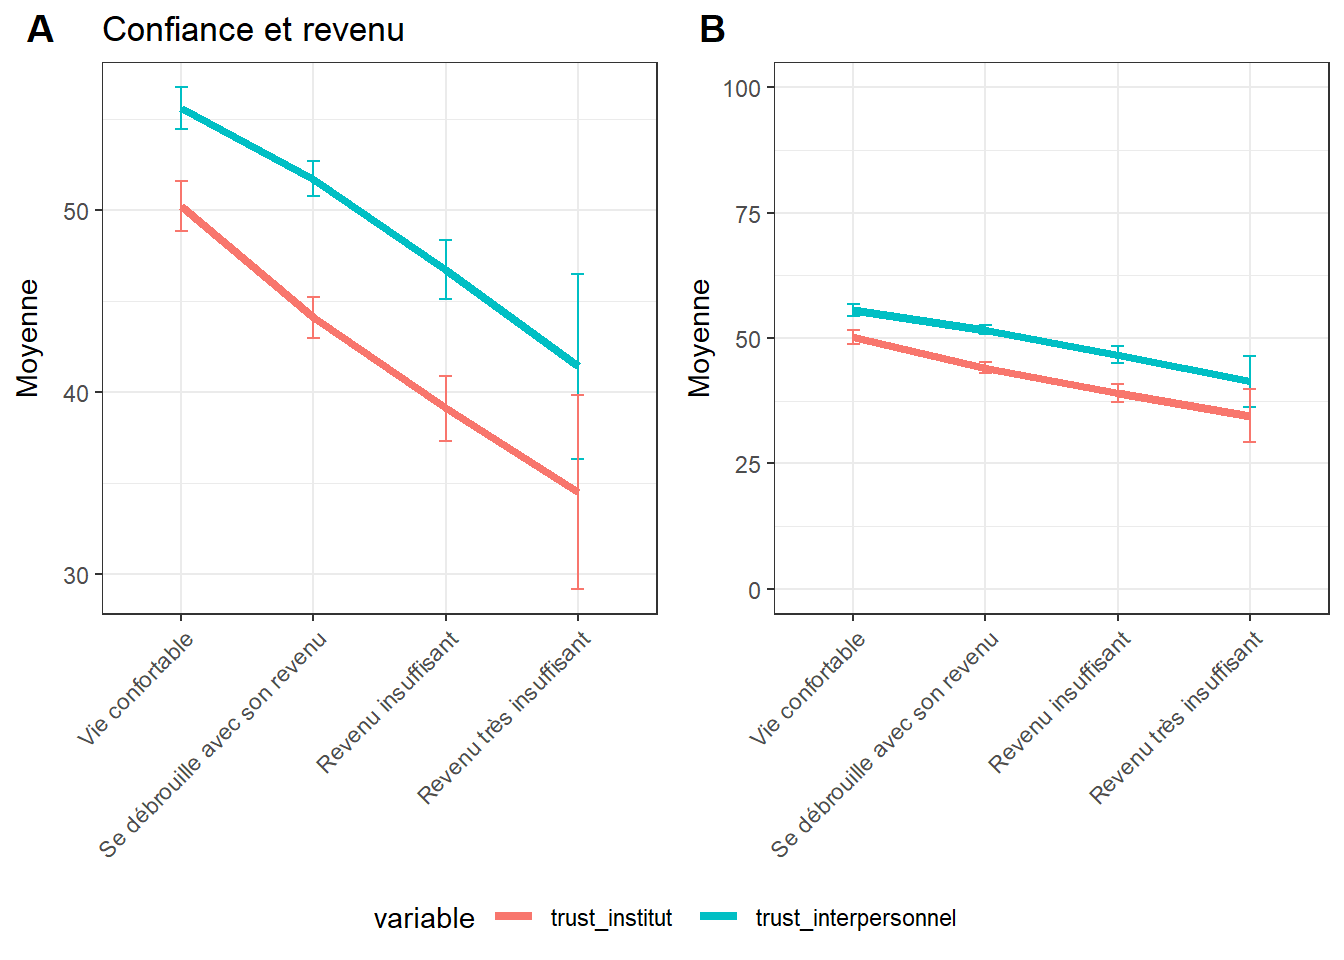
\includegraphics{bookdown-demo_files/figure-latex/321-1.pdf}

La visualisation est utile, encore faut-il qu'on soit bien certain que les variations ne soit pas le produit du hasard, de fluctuations d'échantillonnage. Si en moyenne la perception du pouvoir d'achat est associée à des moyennes de confiance décroissantes, les différences observées sont-elle significatives? Dans les représentations précédentes c'est le choix de l'échelle qui oriente l'analyse.

On a un besoin d'un test plus objectif.Celui est le classique test d'analyse de variance (ANOVA).

Celui-çi est le test d'analyse de variance qui consiste à comparer la variance à l'intérieur des groupes ( intra), et la variance entre les moyennes des groupes ( inter ou between).

\begin{Shaded}
\begin{Highlighting}[]
\NormalTok{foo<-df }\OperatorTok\StringTok{ }
\StringTok{  }\KeywordTok{filter}\NormalTok{(cntry}\OperatorTok{==}\StringTok{"FR"} \OperatorTok{&}\StringTok{ }\NormalTok{Year}\OperatorTok{==}\StringTok{"2018"}\NormalTok{) }\OperatorTok\StringTok{ }\KeywordTok{drop_na}\NormalTok{()}
\NormalTok{fit<-}\KeywordTok{lm}\NormalTok{(trust_institut}\OperatorTok{~}\NormalTok{revenu, foo)}
\KeywordTok{anova}\NormalTok{(fit)}
\end{Highlighting}
\end{Shaded}

\begin{verbatim}
## Analysis of Variance Table
## 
## Response: trust_institut
##             Df Sum Sq Mean Sq F value    Pr(>F)    
## revenu       3  27651  9217.1  32.052 < 2.2e-16 ***
## Residuals 1686 484846   287.6                      
## ---
## Signif. codes:  0 '***' 0.001 '**' 0.01 '*' 0.05 '.' 0.1 ' ' 1
\end{verbatim}

\begin{Shaded}
\begin{Highlighting}[]
\KeywordTok{library}\NormalTok{(xtable)}
\NormalTok{ft <-}\StringTok{ }\KeywordTok{xtable_to_flextable}\NormalTok{(}\KeywordTok{xtable}\NormalTok{(}\KeywordTok{anova}\NormalTok{(fit)), }\DataTypeTok{hline.after =} \KeywordTok{c}\NormalTok{(}\DecValTok{0}\NormalTok{,}\DecValTok{2}\NormalTok{))}
\NormalTok{ft}
\end{Highlighting}
\end{Shaded}

\providecommand{\docline}[3]{\noalign{\global\setlength{\arrayrulewidth}{#1}}\arrayrulecolor[HTML]{#2}\cline{#3}}

\setlength{\tabcolsep}{2pt}

\renewcommand*{\arraystretch}{1.5}

\begin{longtable}[c]{|p{1.01in}|p{0.67in}|p{0.96in}|p{0.91in}|p{0.81in}|p{0.73in}}



\hhline{~~~~~~}

\multicolumn{1}{!{\color[HTML]{000000}\vrule width 0pt}>{\raggedright}p{\dimexpr 1.01in+0\tabcolsep+0\arrayrulewidth}}{\fontsize{11}{11}\selectfont{\textcolor[HTML]{000000}{\global\setmainfont{Arial}{\textbf{}}}}} & \multicolumn{1}{!{\color[HTML]{000000}\vrule width 0pt}>{\raggedleft}p{\dimexpr 0.67in+0\tabcolsep+0\arrayrulewidth}}{\fontsize{11}{11}\selectfont{\textcolor[HTML]{000000}{\global\setmainfont{Arial}{\textbf{Df}}}}} & \multicolumn{1}{!{\color[HTML]{000000}\vrule width 0pt}>{\raggedleft}p{\dimexpr 0.96in+0\tabcolsep+0\arrayrulewidth}}{\fontsize{11}{11}\selectfont{\textcolor[HTML]{000000}{\global\setmainfont{Arial}{\textbf{Sum\ Sq}}}}} & \multicolumn{1}{!{\color[HTML]{000000}\vrule width 0pt}>{\raggedleft}p{\dimexpr 0.91in+0\tabcolsep+0\arrayrulewidth}}{\fontsize{11}{11}\selectfont{\textcolor[HTML]{000000}{\global\setmainfont{Arial}{\textbf{Mean\ Sq}}}}} & \multicolumn{1}{!{\color[HTML]{000000}\vrule width 0pt}>{\raggedleft}p{\dimexpr 0.81in+0\tabcolsep+0\arrayrulewidth}}{\fontsize{11}{11}\selectfont{\textcolor[HTML]{000000}{\global\setmainfont{Arial}{\textbf{F\ value}}}}} & \multicolumn{1}{!{\color[HTML]{000000}\vrule width 0pt}>{\raggedleft}p{\dimexpr 0.73in+0\tabcolsep+0\arrayrulewidth}!{\color[HTML]{000000}\vrule width 0pt}}{\fontsize{11}{11}\selectfont{\textcolor[HTML]{000000}{\global\setmainfont{Arial}{\textbf{Pr(>F)}}}}} \\

\noalign{\global\setlength{\arrayrulewidth}{1pt}}\arrayrulecolor[HTML]{000000}\cline{1-6}

\endfirsthead

\hhline{~~~~~~}

\multicolumn{1}{!{\color[HTML]{000000}\vrule width 0pt}>{\raggedright}p{\dimexpr 1.01in+0\tabcolsep+0\arrayrulewidth}}{\fontsize{11}{11}\selectfont{\textcolor[HTML]{000000}{\global\setmainfont{Arial}{\textbf{}}}}} & \multicolumn{1}{!{\color[HTML]{000000}\vrule width 0pt}>{\raggedleft}p{\dimexpr 0.67in+0\tabcolsep+0\arrayrulewidth}}{\fontsize{11}{11}\selectfont{\textcolor[HTML]{000000}{\global\setmainfont{Arial}{\textbf{Df}}}}} & \multicolumn{1}{!{\color[HTML]{000000}\vrule width 0pt}>{\raggedleft}p{\dimexpr 0.96in+0\tabcolsep+0\arrayrulewidth}}{\fontsize{11}{11}\selectfont{\textcolor[HTML]{000000}{\global\setmainfont{Arial}{\textbf{Sum\ Sq}}}}} & \multicolumn{1}{!{\color[HTML]{000000}\vrule width 0pt}>{\raggedleft}p{\dimexpr 0.91in+0\tabcolsep+0\arrayrulewidth}}{\fontsize{11}{11}\selectfont{\textcolor[HTML]{000000}{\global\setmainfont{Arial}{\textbf{Mean\ Sq}}}}} & \multicolumn{1}{!{\color[HTML]{000000}\vrule width 0pt}>{\raggedleft}p{\dimexpr 0.81in+0\tabcolsep+0\arrayrulewidth}}{\fontsize{11}{11}\selectfont{\textcolor[HTML]{000000}{\global\setmainfont{Arial}{\textbf{F\ value}}}}} & \multicolumn{1}{!{\color[HTML]{000000}\vrule width 0pt}>{\raggedleft}p{\dimexpr 0.73in+0\tabcolsep+0\arrayrulewidth}!{\color[HTML]{000000}\vrule width 0pt}}{\fontsize{11}{11}\selectfont{\textcolor[HTML]{000000}{\global\setmainfont{Arial}{\textbf{Pr(>F)}}}}} \\

\noalign{\global\setlength{\arrayrulewidth}{1pt}}\arrayrulecolor[HTML]{000000}\cline{1-6}\endhead



\multicolumn{1}{!{\color[HTML]{000000}\vrule width 0pt}>{\raggedright}p{\dimexpr 1.01in+0\tabcolsep+0\arrayrulewidth}}{\fontsize{11}{11}\selectfont{\textcolor[HTML]{000000}{\global\setmainfont{Arial}{\textbf{revenu}}}}} & \multicolumn{1}{!{\color[HTML]{000000}\vrule width 0pt}>{\raggedleft}p{\dimexpr 0.67in+0\tabcolsep+0\arrayrulewidth}}{\fontsize{11}{11}\selectfont{\textcolor[HTML]{000000}{\global\setmainfont{Arial}{3}}}} & \multicolumn{1}{!{\color[HTML]{000000}\vrule width 0pt}>{\raggedleft}p{\dimexpr 0.96in+0\tabcolsep+0\arrayrulewidth}}{\fontsize{11}{11}\selectfont{\textcolor[HTML]{000000}{\global\setmainfont{Arial}{27,651.4}}}} & \multicolumn{1}{!{\color[HTML]{000000}\vrule width 0pt}>{\raggedleft}p{\dimexpr 0.91in+0\tabcolsep+0\arrayrulewidth}}{\fontsize{11}{11}\selectfont{\textcolor[HTML]{000000}{\global\setmainfont{Arial}{9,217.1}}}} & \multicolumn{1}{!{\color[HTML]{000000}\vrule width 0pt}>{\raggedleft}p{\dimexpr 0.81in+0\tabcolsep+0\arrayrulewidth}}{\fontsize{11}{11}\selectfont{\textcolor[HTML]{000000}{\global\setmainfont{Arial}{32.1}}}} & \multicolumn{1}{!{\color[HTML]{000000}\vrule width 0pt}>{\raggedleft}p{\dimexpr 0.73in+0\tabcolsep+0\arrayrulewidth}!{\color[HTML]{000000}\vrule width 0pt}}{\fontsize{11}{11}\selectfont{\textcolor[HTML]{000000}{\global\setmainfont{Arial}{0.0}}}} \\





\multicolumn{1}{!{\color[HTML]{000000}\vrule width 0pt}>{\raggedright}p{\dimexpr 1.01in+0\tabcolsep+0\arrayrulewidth}}{\fontsize{11}{11}\selectfont{\textcolor[HTML]{000000}{\global\setmainfont{Arial}{\textbf{Residuals}}}}} & \multicolumn{1}{!{\color[HTML]{000000}\vrule width 0pt}>{\raggedleft}p{\dimexpr 0.67in+0\tabcolsep+0\arrayrulewidth}}{\fontsize{11}{11}\selectfont{\textcolor[HTML]{000000}{\global\setmainfont{Arial}{1,686}}}} & \multicolumn{1}{!{\color[HTML]{000000}\vrule width 0pt}>{\raggedleft}p{\dimexpr 0.96in+0\tabcolsep+0\arrayrulewidth}}{\fontsize{11}{11}\selectfont{\textcolor[HTML]{000000}{\global\setmainfont{Arial}{484,845.7}}}} & \multicolumn{1}{!{\color[HTML]{000000}\vrule width 0pt}>{\raggedleft}p{\dimexpr 0.91in+0\tabcolsep+0\arrayrulewidth}}{\fontsize{11}{11}\selectfont{\textcolor[HTML]{000000}{\global\setmainfont{Arial}{287.6}}}} & \multicolumn{1}{!{\color[HTML]{000000}\vrule width 0pt}>{\raggedleft}p{\dimexpr 0.81in+0\tabcolsep+0\arrayrulewidth}}{\fontsize{11}{11}\selectfont{\textcolor[HTML]{000000}{\global\setmainfont{Arial}{}}}} & \multicolumn{1}{!{\color[HTML]{000000}\vrule width 0pt}>{\raggedleft}p{\dimexpr 0.73in+0\tabcolsep+0\arrayrulewidth}!{\color[HTML]{000000}\vrule width 0pt}}{\fontsize{11}{11}\selectfont{\textcolor[HTML]{000000}{\global\setmainfont{Arial}{}}}} \\

\noalign{\global\setlength{\arrayrulewidth}{1pt}}\arrayrulecolor[HTML]{000000}\cline{1-6}



\end{longtable}

\begin{Shaded}
\begin{Highlighting}[]
\CommentTok{#library(jtools)}
\CommentTok{#summ(fit)}
\CommentTok{#effect_plot(fit, pred="revenu")}
\end{Highlighting}
\end{Shaded}

\hypertarget{deux-variables-qualitatives}{%
\subsection{Deux variables qualitatives}\label{deux-variables-qualitatives}}

L'étude de la relation éventuelle entre deux variables qualitative s'apprécie traditionnellement par une méthode de tableau croisé.

\hypertarget{tableau-croisuxe9}{%
\subsubsection{Tableau croisé}\label{tableau-croisuxe9}}

Pour calculer le tableau croisé on utilise la fonction très simple \texttt{table}.

\begin{Shaded}
\begin{Highlighting}[]
\NormalTok{t<-}\KeywordTok{table}\NormalTok{(foo}\OperatorTok{$}\NormalTok{revenu,foo}\OperatorTok{$}\NormalTok{habitat)}
\NormalTok{t}
\end{Highlighting}
\end{Shaded}

\begin{verbatim}
##                                
##                                 Big city Suburbs Town Village Countryside
##   Vie confortable                    118      82  161     142          31
##   Se débrouille avec son revenu      120     109  275     227          58
##   Revenu insuffisant                  48      38  129      88          22
##   Revenu très insuffisant              9       5   18      10           0
\end{verbatim}

\begin{Shaded}
\begin{Highlighting}[]
\KeywordTok{prop.table}\NormalTok{(t,}\DecValTok{2}\NormalTok{)}
\end{Highlighting}
\end{Shaded}

\begin{verbatim}
##                                
##                                   Big city    Suburbs       Town    Village
##   Vie confortable               0.40000000 0.35042735 0.27615780 0.30406852
##   Se débrouille avec son revenu 0.40677966 0.46581197 0.47169811 0.48608137
##   Revenu insuffisant            0.16271186 0.16239316 0.22126930 0.18843683
##   Revenu très insuffisant       0.03050847 0.02136752 0.03087479 0.02141328
##                                
##                                 Countryside
##   Vie confortable                0.27927928
##   Se débrouille avec son revenu  0.52252252
##   Revenu insuffisant             0.19819820
##   Revenu très insuffisant        0.00000000
\end{verbatim}

Mais ce n'est pas esthétique, de flextable : \texttt{proc\_freq}. Elle nous donne en peu de mots les effectif par cellule, les pourcentages en lignes, et en colonnes.

\begin{Shaded}
\begin{Highlighting}[]
\NormalTok{ft1<-}\StringTok{ }\KeywordTok{proc_freq}\NormalTok{(foo, }\StringTok{"revenu"}\NormalTok{, }\StringTok{"habitat"}\NormalTok{, }\DataTypeTok{include.table_percent =} \OtherTok{FALSE}\NormalTok{,}
                \DataTypeTok{include.row_percent =} \OtherTok{FALSE}\NormalTok{,}
  \DataTypeTok{include.column_percent =} \OtherTok{TRUE}\NormalTok{)}
\NormalTok{ft1}
\end{Highlighting}
\end{Shaded}

\providecommand{\docline}[3]{\noalign{\global\setlength{\arrayrulewidth}{#1}}\arrayrulecolor[HTML]{#2}\cline{#3}}

\setlength{\tabcolsep}{2pt}

\renewcommand*{\arraystretch}{1.5}

\begin{longtable}[c]{|p{2.34in}|p{1.01in}|p{1.26in}|p{1.26in}|p{1.26in}|p{1.26in}|p{1.18in}|p{0.67in}}



\hhline{~~~~~~~~}

\multicolumn{2}{!{\color[HTML]{FFFFFF}\vrule width 0pt}>{\centering}p{\dimexpr 3.35in+2\tabcolsep+1\arrayrulewidth}}{\fontsize{11}{11}\selectfont{\textcolor[HTML]{000000}{\global\setmainfont{Arial}{\textbf{}}}}} & \multicolumn{6}{!{\color[HTML]{FFFFFF}\vrule width 0pt}>{\centering}p{\dimexpr 6.89in+10\tabcolsep+5\arrayrulewidth}!{\color[HTML]{FFFFFF}\vrule width 0pt}}{\fontsize{11}{11}\selectfont{\textcolor[HTML]{000000}{\global\setmainfont{Arial}{\textbf{habitat}}}}} \\

\noalign{\global\setlength{\arrayrulewidth}{1pt}}\arrayrulecolor[HTML]{000000}\cline{1-8}

\multicolumn{1}{!{\color[HTML]{000000}\vrule width 0pt}>{\centering}p{\dimexpr 2.34in+0\tabcolsep+0\arrayrulewidth}}{\fontsize{11}{11}\selectfont{\textcolor[HTML]{000000}{\global\setmainfont{Arial}{\textbf{revenu}}}}} & \multicolumn{1}{!{\color[HTML]{000000}\vrule width 0pt}>{\centering}p{\dimexpr 1.01in+0\tabcolsep+0\arrayrulewidth}}{\fontsize{11}{11}\selectfont{\textcolor[HTML]{000000}{\global\setmainfont{Arial}{\textbf{label}}}}} & \multicolumn{1}{!{\color[HTML]{000000}\vrule width 0pt}>{\centering}p{\dimexpr 1.26in+0\tabcolsep+0\arrayrulewidth}}{\fontsize{11}{11}\selectfont{\textcolor[HTML]{000000}{\global\setmainfont{Arial}{\textbf{Big\ city}}}}} & \multicolumn{1}{!{\color[HTML]{000000}\vrule width 0pt}>{\centering}p{\dimexpr 1.26in+0\tabcolsep+0\arrayrulewidth}}{\fontsize{11}{11}\selectfont{\textcolor[HTML]{000000}{\global\setmainfont{Arial}{\textbf{Suburbs}}}}} & \multicolumn{1}{!{\color[HTML]{000000}\vrule width 0pt}>{\centering}p{\dimexpr 1.26in+0\tabcolsep+0\arrayrulewidth}}{\fontsize{11}{11}\selectfont{\textcolor[HTML]{000000}{\global\setmainfont{Arial}{\textbf{Town}}}}} & \multicolumn{1}{!{\color[HTML]{000000}\vrule width 0pt}>{\centering}p{\dimexpr 1.26in+0\tabcolsep+0\arrayrulewidth}}{\fontsize{11}{11}\selectfont{\textcolor[HTML]{000000}{\global\setmainfont{Arial}{\textbf{Village}}}}} & \multicolumn{1}{!{\color[HTML]{000000}\vrule width 0pt}>{\centering}p{\dimexpr 1.18in+0\tabcolsep+0\arrayrulewidth}}{\fontsize{11}{11}\selectfont{\textcolor[HTML]{000000}{\global\setmainfont{Arial}{\textbf{Countryside}}}}} & \multicolumn{1}{!{\color[HTML]{000000}\vrule width 0pt}>{\centering}p{\dimexpr 0.67in+0\tabcolsep+0\arrayrulewidth}!{\color[HTML]{000000}\vrule width 0pt}}{\fontsize{11}{11}\selectfont{\textcolor[HTML]{000000}{\global\setmainfont{Arial}{\textbf{Total}}}}} \\

\noalign{\global\setlength{\arrayrulewidth}{2pt}}\arrayrulecolor[HTML]{000000}\cline{1-8}

\endfirsthead

\hhline{~~~~~~~~}

\multicolumn{2}{!{\color[HTML]{FFFFFF}\vrule width 0pt}>{\centering}p{\dimexpr 3.35in+2\tabcolsep+1\arrayrulewidth}}{\fontsize{11}{11}\selectfont{\textcolor[HTML]{000000}{\global\setmainfont{Arial}{\textbf{}}}}} & \multicolumn{6}{!{\color[HTML]{FFFFFF}\vrule width 0pt}>{\centering}p{\dimexpr 6.89in+10\tabcolsep+5\arrayrulewidth}!{\color[HTML]{FFFFFF}\vrule width 0pt}}{\fontsize{11}{11}\selectfont{\textcolor[HTML]{000000}{\global\setmainfont{Arial}{\textbf{habitat}}}}} \\

\noalign{\global\setlength{\arrayrulewidth}{1pt}}\arrayrulecolor[HTML]{000000}\cline{1-8}



\multicolumn{1}{!{\color[HTML]{000000}\vrule width 0pt}>{\centering}p{\dimexpr 2.34in+0\tabcolsep+0\arrayrulewidth}}{\fontsize{11}{11}\selectfont{\textcolor[HTML]{000000}{\global\setmainfont{Arial}{\textbf{revenu}}}}} & \multicolumn{1}{!{\color[HTML]{000000}\vrule width 0pt}>{\centering}p{\dimexpr 1.01in+0\tabcolsep+0\arrayrulewidth}}{\fontsize{11}{11}\selectfont{\textcolor[HTML]{000000}{\global\setmainfont{Arial}{\textbf{label}}}}} & \multicolumn{1}{!{\color[HTML]{000000}\vrule width 0pt}>{\centering}p{\dimexpr 1.26in+0\tabcolsep+0\arrayrulewidth}}{\fontsize{11}{11}\selectfont{\textcolor[HTML]{000000}{\global\setmainfont{Arial}{\textbf{Big\ city}}}}} & \multicolumn{1}{!{\color[HTML]{000000}\vrule width 0pt}>{\centering}p{\dimexpr 1.26in+0\tabcolsep+0\arrayrulewidth}}{\fontsize{11}{11}\selectfont{\textcolor[HTML]{000000}{\global\setmainfont{Arial}{\textbf{Suburbs}}}}} & \multicolumn{1}{!{\color[HTML]{000000}\vrule width 0pt}>{\centering}p{\dimexpr 1.26in+0\tabcolsep+0\arrayrulewidth}}{\fontsize{11}{11}\selectfont{\textcolor[HTML]{000000}{\global\setmainfont{Arial}{\textbf{Town}}}}} & \multicolumn{1}{!{\color[HTML]{000000}\vrule width 0pt}>{\centering}p{\dimexpr 1.26in+0\tabcolsep+0\arrayrulewidth}}{\fontsize{11}{11}\selectfont{\textcolor[HTML]{000000}{\global\setmainfont{Arial}{\textbf{Village}}}}} & \multicolumn{1}{!{\color[HTML]{000000}\vrule width 0pt}>{\centering}p{\dimexpr 1.18in+0\tabcolsep+0\arrayrulewidth}}{\fontsize{11}{11}\selectfont{\textcolor[HTML]{000000}{\global\setmainfont{Arial}{\textbf{Countryside}}}}} & \multicolumn{1}{!{\color[HTML]{000000}\vrule width 0pt}>{\centering}p{\dimexpr 0.67in+0\tabcolsep+0\arrayrulewidth}!{\color[HTML]{000000}\vrule width 0pt}}{\fontsize{11}{11}\selectfont{\textcolor[HTML]{000000}{\global\setmainfont{Arial}{\textbf{Total}}}}} \\

\noalign{\global\setlength{\arrayrulewidth}{2pt}}\arrayrulecolor[HTML]{000000}\cline{1-8}\endhead



\multicolumn{1}{!{\color[HTML]{000000}\vrule width 0pt}>{\centering}p{\dimexpr 2.34in+0\tabcolsep+0\arrayrulewidth}}{} & \multicolumn{1}{!{\color[HTML]{000000}\vrule width 0pt}>{\centering}p{\dimexpr 1.01in+0\tabcolsep+0\arrayrulewidth}}{\fontsize{11}{11}\selectfont{\textcolor[HTML]{000000}{\global\setmainfont{Arial}{Frequency}}}} & \multicolumn{1}{!{\color[HTML]{000000}\vrule width 0pt}>{\centering}p{\dimexpr 1.26in+0\tabcolsep+0\arrayrulewidth}}{\fontsize{11}{11}\selectfont{\textcolor[HTML]{000000}{\global\setmainfont{Arial}{118}}}} & \multicolumn{1}{!{\color[HTML]{000000}\vrule width 0pt}>{\centering}p{\dimexpr 1.26in+0\tabcolsep+0\arrayrulewidth}}{\fontsize{11}{11}\selectfont{\textcolor[HTML]{000000}{\global\setmainfont{Arial}{82}}}} & \multicolumn{1}{!{\color[HTML]{000000}\vrule width 0pt}>{\centering}p{\dimexpr 1.26in+0\tabcolsep+0\arrayrulewidth}}{\fontsize{11}{11}\selectfont{\textcolor[HTML]{000000}{\global\setmainfont{Arial}{161}}}} & \multicolumn{1}{!{\color[HTML]{000000}\vrule width 0pt}>{\centering}p{\dimexpr 1.26in+0\tabcolsep+0\arrayrulewidth}}{\fontsize{11}{11}\selectfont{\textcolor[HTML]{000000}{\global\setmainfont{Arial}{142}}}} & \multicolumn{1}{!{\color[HTML]{000000}\vrule width 0pt}>{\centering}p{\dimexpr 1.18in+0\tabcolsep+0\arrayrulewidth}}{\fontsize{11}{11}\selectfont{\textcolor[HTML]{000000}{\global\setmainfont{Arial}{31}}}} & \multicolumn{1}{!{\color[HTML]{000000}\vrule width 0pt}>{\centering}p{\dimexpr 0.67in+0\tabcolsep+0\arrayrulewidth}!{\color[HTML]{000000}\vrule width 0pt}}{\fontsize{11}{11}\selectfont{\textcolor[HTML]{000000}{\global\setmainfont{Arial}{534}}}} \\





\multicolumn{1}{!{\color[HTML]{000000}\vrule width 0pt}>{\centering}p{\dimexpr 2.34in+0\tabcolsep+0\arrayrulewidth}}{\multirow[t]{-2}{*}{\fontsize{11}{11}\selectfont{\textcolor[HTML]{000000}{\global\setmainfont{Arial}{\textbf{Vie\ confortable}}}}}} & \multicolumn{1}{!{\color[HTML]{000000}\vrule width 0pt}>{\centering}p{\dimexpr 1.01in+0\tabcolsep+0\arrayrulewidth}}{\fontsize{11}{11}\selectfont{\textcolor[HTML]{000000}{\global\setmainfont{Arial}{Col\ Pct}}}} & \multicolumn{1}{!{\color[HTML]{000000}\vrule width 0pt}>{\centering}p{\dimexpr 1.26in+0\tabcolsep+0\arrayrulewidth}}{\fontsize{11}{11}\selectfont{\textcolor[HTML]{000000}{\global\setmainfont{Arial}{40\%}}}} & \multicolumn{1}{!{\color[HTML]{000000}\vrule width 0pt}>{\centering}p{\dimexpr 1.26in+0\tabcolsep+0\arrayrulewidth}}{\fontsize{11}{11}\selectfont{\textcolor[HTML]{000000}{\global\setmainfont{Arial}{35.04\%}}}} & \multicolumn{1}{!{\color[HTML]{000000}\vrule width 0pt}>{\centering}p{\dimexpr 1.26in+0\tabcolsep+0\arrayrulewidth}}{\fontsize{11}{11}\selectfont{\textcolor[HTML]{000000}{\global\setmainfont{Arial}{27.62\%}}}} & \multicolumn{1}{!{\color[HTML]{000000}\vrule width 0pt}>{\centering}p{\dimexpr 1.26in+0\tabcolsep+0\arrayrulewidth}}{\fontsize{11}{11}\selectfont{\textcolor[HTML]{000000}{\global\setmainfont{Arial}{30.41\%}}}} & \multicolumn{1}{!{\color[HTML]{000000}\vrule width 0pt}>{\centering}p{\dimexpr 1.18in+0\tabcolsep+0\arrayrulewidth}}{\fontsize{11}{11}\selectfont{\textcolor[HTML]{000000}{\global\setmainfont{Arial}{27.93\%}}}} & \multicolumn{1}{!{\color[HTML]{000000}\vrule width 0pt}>{\centering}p{\dimexpr 0.67in+0\tabcolsep+0\arrayrulewidth}!{\color[HTML]{000000}\vrule width 0pt}}{\fontsize{11}{11}\selectfont{\textcolor[HTML]{000000}{\global\setmainfont{Arial}{}}}} \\





\multicolumn{1}{!{\color[HTML]{000000}\vrule width 0pt}>{\centering}p{\dimexpr 2.34in+0\tabcolsep+0\arrayrulewidth}}{} & \multicolumn{1}{!{\color[HTML]{000000}\vrule width 0pt}>{\centering}p{\dimexpr 1.01in+0\tabcolsep+0\arrayrulewidth}}{\fontsize{11}{11}\selectfont{\textcolor[HTML]{000000}{\global\setmainfont{Arial}{Frequency}}}} & \multicolumn{1}{!{\color[HTML]{000000}\vrule width 0pt}>{\centering}p{\dimexpr 1.26in+0\tabcolsep+0\arrayrulewidth}}{\fontsize{11}{11}\selectfont{\textcolor[HTML]{000000}{\global\setmainfont{Arial}{120}}}} & \multicolumn{1}{!{\color[HTML]{000000}\vrule width 0pt}>{\centering}p{\dimexpr 1.26in+0\tabcolsep+0\arrayrulewidth}}{\fontsize{11}{11}\selectfont{\textcolor[HTML]{000000}{\global\setmainfont{Arial}{109}}}} & \multicolumn{1}{!{\color[HTML]{000000}\vrule width 0pt}>{\centering}p{\dimexpr 1.26in+0\tabcolsep+0\arrayrulewidth}}{\fontsize{11}{11}\selectfont{\textcolor[HTML]{000000}{\global\setmainfont{Arial}{275}}}} & \multicolumn{1}{!{\color[HTML]{000000}\vrule width 0pt}>{\centering}p{\dimexpr 1.26in+0\tabcolsep+0\arrayrulewidth}}{\fontsize{11}{11}\selectfont{\textcolor[HTML]{000000}{\global\setmainfont{Arial}{227}}}} & \multicolumn{1}{!{\color[HTML]{000000}\vrule width 0pt}>{\centering}p{\dimexpr 1.18in+0\tabcolsep+0\arrayrulewidth}}{\fontsize{11}{11}\selectfont{\textcolor[HTML]{000000}{\global\setmainfont{Arial}{58}}}} & \multicolumn{1}{!{\color[HTML]{000000}\vrule width 0pt}>{\centering}p{\dimexpr 0.67in+0\tabcolsep+0\arrayrulewidth}!{\color[HTML]{000000}\vrule width 0pt}}{\fontsize{11}{11}\selectfont{\textcolor[HTML]{000000}{\global\setmainfont{Arial}{789}}}} \\





\multicolumn{1}{!{\color[HTML]{000000}\vrule width 0pt}>{\centering}p{\dimexpr 2.34in+0\tabcolsep+0\arrayrulewidth}}{\multirow[t]{-2}{*}{\fontsize{11}{11}\selectfont{\textcolor[HTML]{000000}{\global\setmainfont{Arial}{\textbf{Se\ débrouille\ avec\ son\ revenu}}}}}} & \multicolumn{1}{!{\color[HTML]{000000}\vrule width 0pt}>{\centering}p{\dimexpr 1.01in+0\tabcolsep+0\arrayrulewidth}}{\fontsize{11}{11}\selectfont{\textcolor[HTML]{000000}{\global\setmainfont{Arial}{Col\ Pct}}}} & \multicolumn{1}{!{\color[HTML]{000000}\vrule width 0pt}>{\centering}p{\dimexpr 1.26in+0\tabcolsep+0\arrayrulewidth}}{\fontsize{11}{11}\selectfont{\textcolor[HTML]{000000}{\global\setmainfont{Arial}{40.68\%}}}} & \multicolumn{1}{!{\color[HTML]{000000}\vrule width 0pt}>{\centering}p{\dimexpr 1.26in+0\tabcolsep+0\arrayrulewidth}}{\fontsize{11}{11}\selectfont{\textcolor[HTML]{000000}{\global\setmainfont{Arial}{46.58\%}}}} & \multicolumn{1}{!{\color[HTML]{000000}\vrule width 0pt}>{\centering}p{\dimexpr 1.26in+0\tabcolsep+0\arrayrulewidth}}{\fontsize{11}{11}\selectfont{\textcolor[HTML]{000000}{\global\setmainfont{Arial}{47.17\%}}}} & \multicolumn{1}{!{\color[HTML]{000000}\vrule width 0pt}>{\centering}p{\dimexpr 1.26in+0\tabcolsep+0\arrayrulewidth}}{\fontsize{11}{11}\selectfont{\textcolor[HTML]{000000}{\global\setmainfont{Arial}{48.61\%}}}} & \multicolumn{1}{!{\color[HTML]{000000}\vrule width 0pt}>{\centering}p{\dimexpr 1.18in+0\tabcolsep+0\arrayrulewidth}}{\fontsize{11}{11}\selectfont{\textcolor[HTML]{000000}{\global\setmainfont{Arial}{52.25\%}}}} & \multicolumn{1}{!{\color[HTML]{000000}\vrule width 0pt}>{\centering}p{\dimexpr 0.67in+0\tabcolsep+0\arrayrulewidth}!{\color[HTML]{000000}\vrule width 0pt}}{\fontsize{11}{11}\selectfont{\textcolor[HTML]{000000}{\global\setmainfont{Arial}{}}}} \\





\multicolumn{1}{!{\color[HTML]{000000}\vrule width 0pt}>{\centering}p{\dimexpr 2.34in+0\tabcolsep+0\arrayrulewidth}}{} & \multicolumn{1}{!{\color[HTML]{000000}\vrule width 0pt}>{\centering}p{\dimexpr 1.01in+0\tabcolsep+0\arrayrulewidth}}{\fontsize{11}{11}\selectfont{\textcolor[HTML]{000000}{\global\setmainfont{Arial}{Frequency}}}} & \multicolumn{1}{!{\color[HTML]{000000}\vrule width 0pt}>{\centering}p{\dimexpr 1.26in+0\tabcolsep+0\arrayrulewidth}}{\fontsize{11}{11}\selectfont{\textcolor[HTML]{000000}{\global\setmainfont{Arial}{48}}}} & \multicolumn{1}{!{\color[HTML]{000000}\vrule width 0pt}>{\centering}p{\dimexpr 1.26in+0\tabcolsep+0\arrayrulewidth}}{\fontsize{11}{11}\selectfont{\textcolor[HTML]{000000}{\global\setmainfont{Arial}{38}}}} & \multicolumn{1}{!{\color[HTML]{000000}\vrule width 0pt}>{\centering}p{\dimexpr 1.26in+0\tabcolsep+0\arrayrulewidth}}{\fontsize{11}{11}\selectfont{\textcolor[HTML]{000000}{\global\setmainfont{Arial}{129}}}} & \multicolumn{1}{!{\color[HTML]{000000}\vrule width 0pt}>{\centering}p{\dimexpr 1.26in+0\tabcolsep+0\arrayrulewidth}}{\fontsize{11}{11}\selectfont{\textcolor[HTML]{000000}{\global\setmainfont{Arial}{88}}}} & \multicolumn{1}{!{\color[HTML]{000000}\vrule width 0pt}>{\centering}p{\dimexpr 1.18in+0\tabcolsep+0\arrayrulewidth}}{\fontsize{11}{11}\selectfont{\textcolor[HTML]{000000}{\global\setmainfont{Arial}{22}}}} & \multicolumn{1}{!{\color[HTML]{000000}\vrule width 0pt}>{\centering}p{\dimexpr 0.67in+0\tabcolsep+0\arrayrulewidth}!{\color[HTML]{000000}\vrule width 0pt}}{\fontsize{11}{11}\selectfont{\textcolor[HTML]{000000}{\global\setmainfont{Arial}{325}}}} \\





\multicolumn{1}{!{\color[HTML]{000000}\vrule width 0pt}>{\centering}p{\dimexpr 2.34in+0\tabcolsep+0\arrayrulewidth}}{\multirow[t]{-2}{*}{\fontsize{11}{11}\selectfont{\textcolor[HTML]{000000}{\global\setmainfont{Arial}{\textbf{Revenu\ insuffisant}}}}}} & \multicolumn{1}{!{\color[HTML]{000000}\vrule width 0pt}>{\centering}p{\dimexpr 1.01in+0\tabcolsep+0\arrayrulewidth}}{\fontsize{11}{11}\selectfont{\textcolor[HTML]{000000}{\global\setmainfont{Arial}{Col\ Pct}}}} & \multicolumn{1}{!{\color[HTML]{000000}\vrule width 0pt}>{\centering}p{\dimexpr 1.26in+0\tabcolsep+0\arrayrulewidth}}{\fontsize{11}{11}\selectfont{\textcolor[HTML]{000000}{\global\setmainfont{Arial}{16.27\%}}}} & \multicolumn{1}{!{\color[HTML]{000000}\vrule width 0pt}>{\centering}p{\dimexpr 1.26in+0\tabcolsep+0\arrayrulewidth}}{\fontsize{11}{11}\selectfont{\textcolor[HTML]{000000}{\global\setmainfont{Arial}{16.24\%}}}} & \multicolumn{1}{!{\color[HTML]{000000}\vrule width 0pt}>{\centering}p{\dimexpr 1.26in+0\tabcolsep+0\arrayrulewidth}}{\fontsize{11}{11}\selectfont{\textcolor[HTML]{000000}{\global\setmainfont{Arial}{22.13\%}}}} & \multicolumn{1}{!{\color[HTML]{000000}\vrule width 0pt}>{\centering}p{\dimexpr 1.26in+0\tabcolsep+0\arrayrulewidth}}{\fontsize{11}{11}\selectfont{\textcolor[HTML]{000000}{\global\setmainfont{Arial}{18.84\%}}}} & \multicolumn{1}{!{\color[HTML]{000000}\vrule width 0pt}>{\centering}p{\dimexpr 1.18in+0\tabcolsep+0\arrayrulewidth}}{\fontsize{11}{11}\selectfont{\textcolor[HTML]{000000}{\global\setmainfont{Arial}{19.82\%}}}} & \multicolumn{1}{!{\color[HTML]{000000}\vrule width 0pt}>{\centering}p{\dimexpr 0.67in+0\tabcolsep+0\arrayrulewidth}!{\color[HTML]{000000}\vrule width 0pt}}{\fontsize{11}{11}\selectfont{\textcolor[HTML]{000000}{\global\setmainfont{Arial}{}}}} \\





\multicolumn{1}{!{\color[HTML]{000000}\vrule width 0pt}>{\centering}p{\dimexpr 2.34in+0\tabcolsep+0\arrayrulewidth}}{} & \multicolumn{1}{!{\color[HTML]{000000}\vrule width 0pt}>{\centering}p{\dimexpr 1.01in+0\tabcolsep+0\arrayrulewidth}}{\fontsize{11}{11}\selectfont{\textcolor[HTML]{000000}{\global\setmainfont{Arial}{Frequency}}}} & \multicolumn{1}{!{\color[HTML]{000000}\vrule width 0pt}>{\centering}p{\dimexpr 1.26in+0\tabcolsep+0\arrayrulewidth}}{\fontsize{11}{11}\selectfont{\textcolor[HTML]{000000}{\global\setmainfont{Arial}{9}}}} & \multicolumn{1}{!{\color[HTML]{000000}\vrule width 0pt}>{\centering}p{\dimexpr 1.26in+0\tabcolsep+0\arrayrulewidth}}{\fontsize{11}{11}\selectfont{\textcolor[HTML]{000000}{\global\setmainfont{Arial}{5}}}} & \multicolumn{1}{!{\color[HTML]{000000}\vrule width 0pt}>{\centering}p{\dimexpr 1.26in+0\tabcolsep+0\arrayrulewidth}}{\fontsize{11}{11}\selectfont{\textcolor[HTML]{000000}{\global\setmainfont{Arial}{18}}}} & \multicolumn{1}{!{\color[HTML]{000000}\vrule width 0pt}>{\centering}p{\dimexpr 1.26in+0\tabcolsep+0\arrayrulewidth}}{\fontsize{11}{11}\selectfont{\textcolor[HTML]{000000}{\global\setmainfont{Arial}{10}}}} & \multicolumn{1}{!{\color[HTML]{000000}\vrule width 0pt}>{\centering}p{\dimexpr 1.18in+0\tabcolsep+0\arrayrulewidth}}{\fontsize{11}{11}\selectfont{\textcolor[HTML]{000000}{\global\setmainfont{Arial}{0}}}} & \multicolumn{1}{!{\color[HTML]{000000}\vrule width 0pt}>{\centering}p{\dimexpr 0.67in+0\tabcolsep+0\arrayrulewidth}!{\color[HTML]{000000}\vrule width 0pt}}{\fontsize{11}{11}\selectfont{\textcolor[HTML]{000000}{\global\setmainfont{Arial}{42}}}} \\





\multicolumn{1}{!{\color[HTML]{000000}\vrule width 0pt}>{\centering}p{\dimexpr 2.34in+0\tabcolsep+0\arrayrulewidth}}{\multirow[t]{-2}{*}{\fontsize{11}{11}\selectfont{\textcolor[HTML]{000000}{\global\setmainfont{Arial}{\textbf{Revenu\ très\ insuffisant}}}}}} & \multicolumn{1}{!{\color[HTML]{000000}\vrule width 0pt}>{\centering}p{\dimexpr 1.01in+0\tabcolsep+0\arrayrulewidth}}{\fontsize{11}{11}\selectfont{\textcolor[HTML]{000000}{\global\setmainfont{Arial}{Col\ Pct}}}} & \multicolumn{1}{!{\color[HTML]{000000}\vrule width 0pt}>{\centering}p{\dimexpr 1.26in+0\tabcolsep+0\arrayrulewidth}}{\fontsize{11}{11}\selectfont{\textcolor[HTML]{000000}{\global\setmainfont{Arial}{3.05\%}}}} & \multicolumn{1}{!{\color[HTML]{000000}\vrule width 0pt}>{\centering}p{\dimexpr 1.26in+0\tabcolsep+0\arrayrulewidth}}{\fontsize{11}{11}\selectfont{\textcolor[HTML]{000000}{\global\setmainfont{Arial}{2.14\%}}}} & \multicolumn{1}{!{\color[HTML]{000000}\vrule width 0pt}>{\centering}p{\dimexpr 1.26in+0\tabcolsep+0\arrayrulewidth}}{\fontsize{11}{11}\selectfont{\textcolor[HTML]{000000}{\global\setmainfont{Arial}{3.09\%}}}} & \multicolumn{1}{!{\color[HTML]{000000}\vrule width 0pt}>{\centering}p{\dimexpr 1.26in+0\tabcolsep+0\arrayrulewidth}}{\fontsize{11}{11}\selectfont{\textcolor[HTML]{000000}{\global\setmainfont{Arial}{2.14\%}}}} & \multicolumn{1}{!{\color[HTML]{000000}\vrule width 0pt}>{\centering}p{\dimexpr 1.18in+0\tabcolsep+0\arrayrulewidth}}{\fontsize{11}{11}\selectfont{\textcolor[HTML]{000000}{\global\setmainfont{Arial}{0\%}}}} & \multicolumn{1}{!{\color[HTML]{000000}\vrule width 0pt}>{\centering}p{\dimexpr 0.67in+0\tabcolsep+0\arrayrulewidth}!{\color[HTML]{000000}\vrule width 0pt}}{\fontsize{11}{11}\selectfont{\textcolor[HTML]{000000}{\global\setmainfont{Arial}{}}}} \\





\multicolumn{1}{!{\color[HTML]{000000}\vrule width 0pt}>{\centering}p{\dimexpr 2.34in+0\tabcolsep+0\arrayrulewidth}}{\fontsize{11}{11}\selectfont{\textcolor[HTML]{000000}{\global\setmainfont{Arial}{\textbf{Total}}}}} & \multicolumn{1}{!{\color[HTML]{000000}\vrule width 0pt}>{\centering}p{\dimexpr 1.01in+0\tabcolsep+0\arrayrulewidth}}{\fontsize{11}{11}\selectfont{\textcolor[HTML]{000000}{\global\setmainfont{Arial}{Frequency}}}} & \multicolumn{1}{!{\color[HTML]{000000}\vrule width 0pt}>{\centering}p{\dimexpr 1.26in+0\tabcolsep+0\arrayrulewidth}}{\fontsize{11}{11}\selectfont{\textcolor[HTML]{000000}{\global\setmainfont{Arial}{295}}}} & \multicolumn{1}{!{\color[HTML]{000000}\vrule width 0pt}>{\centering}p{\dimexpr 1.26in+0\tabcolsep+0\arrayrulewidth}}{\fontsize{11}{11}\selectfont{\textcolor[HTML]{000000}{\global\setmainfont{Arial}{234}}}} & \multicolumn{1}{!{\color[HTML]{000000}\vrule width 0pt}>{\centering}p{\dimexpr 1.26in+0\tabcolsep+0\arrayrulewidth}}{\fontsize{11}{11}\selectfont{\textcolor[HTML]{000000}{\global\setmainfont{Arial}{583}}}} & \multicolumn{1}{!{\color[HTML]{000000}\vrule width 0pt}>{\centering}p{\dimexpr 1.26in+0\tabcolsep+0\arrayrulewidth}}{\fontsize{11}{11}\selectfont{\textcolor[HTML]{000000}{\global\setmainfont{Arial}{467}}}} & \multicolumn{1}{!{\color[HTML]{000000}\vrule width 0pt}>{\centering}p{\dimexpr 1.18in+0\tabcolsep+0\arrayrulewidth}}{\fontsize{11}{11}\selectfont{\textcolor[HTML]{000000}{\global\setmainfont{Arial}{111}}}} & \multicolumn{1}{!{\color[HTML]{000000}\vrule width 0pt}>{\centering}p{\dimexpr 0.67in+0\tabcolsep+0\arrayrulewidth}!{\color[HTML]{000000}\vrule width 0pt}}{\fontsize{11}{11}\selectfont{\textcolor[HTML]{000000}{\global\setmainfont{Arial}{1690}}}} \\

\noalign{\global\setlength{\arrayrulewidth}{2pt}}\arrayrulecolor[HTML]{666666}\cline{1-8}



\end{longtable}

\begin{Shaded}
\begin{Highlighting}[]
\NormalTok{ft2<-}\StringTok{ }\KeywordTok{proc_freq}\NormalTok{(foo, }\StringTok{"revenu"}\NormalTok{, }\StringTok{"habitat"}\NormalTok{, }\DataTypeTok{include.table_percent =} \OtherTok{FALSE}\NormalTok{,}
                \DataTypeTok{include.row_percent =} \OtherTok{TRUE}\NormalTok{,}
  \DataTypeTok{include.column_percent =} \OtherTok{FALSE}\NormalTok{)}
\NormalTok{ft2}
\end{Highlighting}
\end{Shaded}

\providecommand{\docline}[3]{\noalign{\global\setlength{\arrayrulewidth}{#1}}\arrayrulecolor[HTML]{#2}\cline{#3}}

\setlength{\tabcolsep}{2pt}

\renewcommand*{\arraystretch}{1.5}

\begin{longtable}[c]{|p{2.34in}|p{1.01in}|p{1.18in}|p{1.18in}|p{1.18in}|p{1.18in}|p{1.26in}|p{0.67in}}



\hhline{~~~~~~~~}

\multicolumn{2}{!{\color[HTML]{FFFFFF}\vrule width 0pt}>{\centering}p{\dimexpr 3.35in+2\tabcolsep+1\arrayrulewidth}}{\fontsize{11}{11}\selectfont{\textcolor[HTML]{000000}{\global\setmainfont{Arial}{\textbf{}}}}} & \multicolumn{6}{!{\color[HTML]{FFFFFF}\vrule width 0pt}>{\centering}p{\dimexpr 6.64in+10\tabcolsep+5\arrayrulewidth}!{\color[HTML]{FFFFFF}\vrule width 0pt}}{\fontsize{11}{11}\selectfont{\textcolor[HTML]{000000}{\global\setmainfont{Arial}{\textbf{habitat}}}}} \\

\noalign{\global\setlength{\arrayrulewidth}{1pt}}\arrayrulecolor[HTML]{000000}\cline{1-8}

\multicolumn{1}{!{\color[HTML]{000000}\vrule width 0pt}>{\centering}p{\dimexpr 2.34in+0\tabcolsep+0\arrayrulewidth}}{\fontsize{11}{11}\selectfont{\textcolor[HTML]{000000}{\global\setmainfont{Arial}{\textbf{revenu}}}}} & \multicolumn{1}{!{\color[HTML]{000000}\vrule width 0pt}>{\centering}p{\dimexpr 1.01in+0\tabcolsep+0\arrayrulewidth}}{\fontsize{11}{11}\selectfont{\textcolor[HTML]{000000}{\global\setmainfont{Arial}{\textbf{label}}}}} & \multicolumn{1}{!{\color[HTML]{000000}\vrule width 0pt}>{\centering}p{\dimexpr 1.18in+0\tabcolsep+0\arrayrulewidth}}{\fontsize{11}{11}\selectfont{\textcolor[HTML]{000000}{\global\setmainfont{Arial}{\textbf{Big\ city}}}}} & \multicolumn{1}{!{\color[HTML]{000000}\vrule width 0pt}>{\centering}p{\dimexpr 1.18in+0\tabcolsep+0\arrayrulewidth}}{\fontsize{11}{11}\selectfont{\textcolor[HTML]{000000}{\global\setmainfont{Arial}{\textbf{Suburbs}}}}} & \multicolumn{1}{!{\color[HTML]{000000}\vrule width 0pt}>{\centering}p{\dimexpr 1.18in+0\tabcolsep+0\arrayrulewidth}}{\fontsize{11}{11}\selectfont{\textcolor[HTML]{000000}{\global\setmainfont{Arial}{\textbf{Town}}}}} & \multicolumn{1}{!{\color[HTML]{000000}\vrule width 0pt}>{\centering}p{\dimexpr 1.18in+0\tabcolsep+0\arrayrulewidth}}{\fontsize{11}{11}\selectfont{\textcolor[HTML]{000000}{\global\setmainfont{Arial}{\textbf{Village}}}}} & \multicolumn{1}{!{\color[HTML]{000000}\vrule width 0pt}>{\centering}p{\dimexpr 1.26in+0\tabcolsep+0\arrayrulewidth}}{\fontsize{11}{11}\selectfont{\textcolor[HTML]{000000}{\global\setmainfont{Arial}{\textbf{Countryside}}}}} & \multicolumn{1}{!{\color[HTML]{000000}\vrule width 0pt}>{\centering}p{\dimexpr 0.67in+0\tabcolsep+0\arrayrulewidth}!{\color[HTML]{000000}\vrule width 0pt}}{\fontsize{11}{11}\selectfont{\textcolor[HTML]{000000}{\global\setmainfont{Arial}{\textbf{Total}}}}} \\

\noalign{\global\setlength{\arrayrulewidth}{2pt}}\arrayrulecolor[HTML]{000000}\cline{1-8}

\endfirsthead

\hhline{~~~~~~~~}

\multicolumn{2}{!{\color[HTML]{FFFFFF}\vrule width 0pt}>{\centering}p{\dimexpr 3.35in+2\tabcolsep+1\arrayrulewidth}}{\fontsize{11}{11}\selectfont{\textcolor[HTML]{000000}{\global\setmainfont{Arial}{\textbf{}}}}} & \multicolumn{6}{!{\color[HTML]{FFFFFF}\vrule width 0pt}>{\centering}p{\dimexpr 6.64in+10\tabcolsep+5\arrayrulewidth}!{\color[HTML]{FFFFFF}\vrule width 0pt}}{\fontsize{11}{11}\selectfont{\textcolor[HTML]{000000}{\global\setmainfont{Arial}{\textbf{habitat}}}}} \\

\noalign{\global\setlength{\arrayrulewidth}{1pt}}\arrayrulecolor[HTML]{000000}\cline{1-8}



\multicolumn{1}{!{\color[HTML]{000000}\vrule width 0pt}>{\centering}p{\dimexpr 2.34in+0\tabcolsep+0\arrayrulewidth}}{\fontsize{11}{11}\selectfont{\textcolor[HTML]{000000}{\global\setmainfont{Arial}{\textbf{revenu}}}}} & \multicolumn{1}{!{\color[HTML]{000000}\vrule width 0pt}>{\centering}p{\dimexpr 1.01in+0\tabcolsep+0\arrayrulewidth}}{\fontsize{11}{11}\selectfont{\textcolor[HTML]{000000}{\global\setmainfont{Arial}{\textbf{label}}}}} & \multicolumn{1}{!{\color[HTML]{000000}\vrule width 0pt}>{\centering}p{\dimexpr 1.18in+0\tabcolsep+0\arrayrulewidth}}{\fontsize{11}{11}\selectfont{\textcolor[HTML]{000000}{\global\setmainfont{Arial}{\textbf{Big\ city}}}}} & \multicolumn{1}{!{\color[HTML]{000000}\vrule width 0pt}>{\centering}p{\dimexpr 1.18in+0\tabcolsep+0\arrayrulewidth}}{\fontsize{11}{11}\selectfont{\textcolor[HTML]{000000}{\global\setmainfont{Arial}{\textbf{Suburbs}}}}} & \multicolumn{1}{!{\color[HTML]{000000}\vrule width 0pt}>{\centering}p{\dimexpr 1.18in+0\tabcolsep+0\arrayrulewidth}}{\fontsize{11}{11}\selectfont{\textcolor[HTML]{000000}{\global\setmainfont{Arial}{\textbf{Town}}}}} & \multicolumn{1}{!{\color[HTML]{000000}\vrule width 0pt}>{\centering}p{\dimexpr 1.18in+0\tabcolsep+0\arrayrulewidth}}{\fontsize{11}{11}\selectfont{\textcolor[HTML]{000000}{\global\setmainfont{Arial}{\textbf{Village}}}}} & \multicolumn{1}{!{\color[HTML]{000000}\vrule width 0pt}>{\centering}p{\dimexpr 1.26in+0\tabcolsep+0\arrayrulewidth}}{\fontsize{11}{11}\selectfont{\textcolor[HTML]{000000}{\global\setmainfont{Arial}{\textbf{Countryside}}}}} & \multicolumn{1}{!{\color[HTML]{000000}\vrule width 0pt}>{\centering}p{\dimexpr 0.67in+0\tabcolsep+0\arrayrulewidth}!{\color[HTML]{000000}\vrule width 0pt}}{\fontsize{11}{11}\selectfont{\textcolor[HTML]{000000}{\global\setmainfont{Arial}{\textbf{Total}}}}} \\

\noalign{\global\setlength{\arrayrulewidth}{2pt}}\arrayrulecolor[HTML]{000000}\cline{1-8}\endhead



\multicolumn{1}{!{\color[HTML]{000000}\vrule width 0pt}>{\centering}p{\dimexpr 2.34in+0\tabcolsep+0\arrayrulewidth}}{} & \multicolumn{1}{!{\color[HTML]{000000}\vrule width 0pt}>{\centering}p{\dimexpr 1.01in+0\tabcolsep+0\arrayrulewidth}}{\fontsize{11}{11}\selectfont{\textcolor[HTML]{000000}{\global\setmainfont{Arial}{Frequency}}}} & \multicolumn{1}{!{\color[HTML]{000000}\vrule width 0pt}>{\centering}p{\dimexpr 1.18in+0\tabcolsep+0\arrayrulewidth}}{\fontsize{11}{11}\selectfont{\textcolor[HTML]{000000}{\global\setmainfont{Arial}{118}}}} & \multicolumn{1}{!{\color[HTML]{000000}\vrule width 0pt}>{\centering}p{\dimexpr 1.18in+0\tabcolsep+0\arrayrulewidth}}{\fontsize{11}{11}\selectfont{\textcolor[HTML]{000000}{\global\setmainfont{Arial}{82}}}} & \multicolumn{1}{!{\color[HTML]{000000}\vrule width 0pt}>{\centering}p{\dimexpr 1.18in+0\tabcolsep+0\arrayrulewidth}}{\fontsize{11}{11}\selectfont{\textcolor[HTML]{000000}{\global\setmainfont{Arial}{161}}}} & \multicolumn{1}{!{\color[HTML]{000000}\vrule width 0pt}>{\centering}p{\dimexpr 1.18in+0\tabcolsep+0\arrayrulewidth}}{\fontsize{11}{11}\selectfont{\textcolor[HTML]{000000}{\global\setmainfont{Arial}{142}}}} & \multicolumn{1}{!{\color[HTML]{000000}\vrule width 0pt}>{\centering}p{\dimexpr 1.26in+0\tabcolsep+0\arrayrulewidth}}{\fontsize{11}{11}\selectfont{\textcolor[HTML]{000000}{\global\setmainfont{Arial}{31}}}} & \multicolumn{1}{!{\color[HTML]{000000}\vrule width 0pt}>{\centering}p{\dimexpr 0.67in+0\tabcolsep+0\arrayrulewidth}!{\color[HTML]{000000}\vrule width 0pt}}{\fontsize{11}{11}\selectfont{\textcolor[HTML]{000000}{\global\setmainfont{Arial}{534}}}} \\





\multicolumn{1}{!{\color[HTML]{000000}\vrule width 0pt}>{\centering}p{\dimexpr 2.34in+0\tabcolsep+0\arrayrulewidth}}{\multirow[t]{-2}{*}{\fontsize{11}{11}\selectfont{\textcolor[HTML]{000000}{\global\setmainfont{Arial}{\textbf{Vie\ confortable}}}}}} & \multicolumn{1}{!{\color[HTML]{000000}\vrule width 0pt}>{\centering}p{\dimexpr 1.01in+0\tabcolsep+0\arrayrulewidth}}{\fontsize{11}{11}\selectfont{\textcolor[HTML]{000000}{\global\setmainfont{Arial}{Row\ Pct}}}} & \multicolumn{1}{!{\color[HTML]{000000}\vrule width 0pt}>{\centering}p{\dimexpr 1.18in+0\tabcolsep+0\arrayrulewidth}}{\fontsize{11}{11}\selectfont{\textcolor[HTML]{000000}{\global\setmainfont{Arial}{22.1\%}}}} & \multicolumn{1}{!{\color[HTML]{000000}\vrule width 0pt}>{\centering}p{\dimexpr 1.18in+0\tabcolsep+0\arrayrulewidth}}{\fontsize{11}{11}\selectfont{\textcolor[HTML]{000000}{\global\setmainfont{Arial}{15.36\%}}}} & \multicolumn{1}{!{\color[HTML]{000000}\vrule width 0pt}>{\centering}p{\dimexpr 1.18in+0\tabcolsep+0\arrayrulewidth}}{\fontsize{11}{11}\selectfont{\textcolor[HTML]{000000}{\global\setmainfont{Arial}{30.15\%}}}} & \multicolumn{1}{!{\color[HTML]{000000}\vrule width 0pt}>{\centering}p{\dimexpr 1.18in+0\tabcolsep+0\arrayrulewidth}}{\fontsize{11}{11}\selectfont{\textcolor[HTML]{000000}{\global\setmainfont{Arial}{26.59\%}}}} & \multicolumn{1}{!{\color[HTML]{000000}\vrule width 0pt}>{\centering}p{\dimexpr 1.26in+0\tabcolsep+0\arrayrulewidth}}{\fontsize{11}{11}\selectfont{\textcolor[HTML]{000000}{\global\setmainfont{Arial}{5.81\%}}}} & \multicolumn{1}{!{\color[HTML]{000000}\vrule width 0pt}>{\centering}p{\dimexpr 0.67in+0\tabcolsep+0\arrayrulewidth}!{\color[HTML]{000000}\vrule width 0pt}}{\fontsize{11}{11}\selectfont{\textcolor[HTML]{000000}{\global\setmainfont{Arial}{}}}} \\





\multicolumn{1}{!{\color[HTML]{000000}\vrule width 0pt}>{\centering}p{\dimexpr 2.34in+0\tabcolsep+0\arrayrulewidth}}{} & \multicolumn{1}{!{\color[HTML]{000000}\vrule width 0pt}>{\centering}p{\dimexpr 1.01in+0\tabcolsep+0\arrayrulewidth}}{\fontsize{11}{11}\selectfont{\textcolor[HTML]{000000}{\global\setmainfont{Arial}{Frequency}}}} & \multicolumn{1}{!{\color[HTML]{000000}\vrule width 0pt}>{\centering}p{\dimexpr 1.18in+0\tabcolsep+0\arrayrulewidth}}{\fontsize{11}{11}\selectfont{\textcolor[HTML]{000000}{\global\setmainfont{Arial}{120}}}} & \multicolumn{1}{!{\color[HTML]{000000}\vrule width 0pt}>{\centering}p{\dimexpr 1.18in+0\tabcolsep+0\arrayrulewidth}}{\fontsize{11}{11}\selectfont{\textcolor[HTML]{000000}{\global\setmainfont{Arial}{109}}}} & \multicolumn{1}{!{\color[HTML]{000000}\vrule width 0pt}>{\centering}p{\dimexpr 1.18in+0\tabcolsep+0\arrayrulewidth}}{\fontsize{11}{11}\selectfont{\textcolor[HTML]{000000}{\global\setmainfont{Arial}{275}}}} & \multicolumn{1}{!{\color[HTML]{000000}\vrule width 0pt}>{\centering}p{\dimexpr 1.18in+0\tabcolsep+0\arrayrulewidth}}{\fontsize{11}{11}\selectfont{\textcolor[HTML]{000000}{\global\setmainfont{Arial}{227}}}} & \multicolumn{1}{!{\color[HTML]{000000}\vrule width 0pt}>{\centering}p{\dimexpr 1.26in+0\tabcolsep+0\arrayrulewidth}}{\fontsize{11}{11}\selectfont{\textcolor[HTML]{000000}{\global\setmainfont{Arial}{58}}}} & \multicolumn{1}{!{\color[HTML]{000000}\vrule width 0pt}>{\centering}p{\dimexpr 0.67in+0\tabcolsep+0\arrayrulewidth}!{\color[HTML]{000000}\vrule width 0pt}}{\fontsize{11}{11}\selectfont{\textcolor[HTML]{000000}{\global\setmainfont{Arial}{789}}}} \\





\multicolumn{1}{!{\color[HTML]{000000}\vrule width 0pt}>{\centering}p{\dimexpr 2.34in+0\tabcolsep+0\arrayrulewidth}}{\multirow[t]{-2}{*}{\fontsize{11}{11}\selectfont{\textcolor[HTML]{000000}{\global\setmainfont{Arial}{\textbf{Se\ débrouille\ avec\ son\ revenu}}}}}} & \multicolumn{1}{!{\color[HTML]{000000}\vrule width 0pt}>{\centering}p{\dimexpr 1.01in+0\tabcolsep+0\arrayrulewidth}}{\fontsize{11}{11}\selectfont{\textcolor[HTML]{000000}{\global\setmainfont{Arial}{Row\ Pct}}}} & \multicolumn{1}{!{\color[HTML]{000000}\vrule width 0pt}>{\centering}p{\dimexpr 1.18in+0\tabcolsep+0\arrayrulewidth}}{\fontsize{11}{11}\selectfont{\textcolor[HTML]{000000}{\global\setmainfont{Arial}{15.21\%}}}} & \multicolumn{1}{!{\color[HTML]{000000}\vrule width 0pt}>{\centering}p{\dimexpr 1.18in+0\tabcolsep+0\arrayrulewidth}}{\fontsize{11}{11}\selectfont{\textcolor[HTML]{000000}{\global\setmainfont{Arial}{13.81\%}}}} & \multicolumn{1}{!{\color[HTML]{000000}\vrule width 0pt}>{\centering}p{\dimexpr 1.18in+0\tabcolsep+0\arrayrulewidth}}{\fontsize{11}{11}\selectfont{\textcolor[HTML]{000000}{\global\setmainfont{Arial}{34.85\%}}}} & \multicolumn{1}{!{\color[HTML]{000000}\vrule width 0pt}>{\centering}p{\dimexpr 1.18in+0\tabcolsep+0\arrayrulewidth}}{\fontsize{11}{11}\selectfont{\textcolor[HTML]{000000}{\global\setmainfont{Arial}{28.77\%}}}} & \multicolumn{1}{!{\color[HTML]{000000}\vrule width 0pt}>{\centering}p{\dimexpr 1.26in+0\tabcolsep+0\arrayrulewidth}}{\fontsize{11}{11}\selectfont{\textcolor[HTML]{000000}{\global\setmainfont{Arial}{7.35\%}}}} & \multicolumn{1}{!{\color[HTML]{000000}\vrule width 0pt}>{\centering}p{\dimexpr 0.67in+0\tabcolsep+0\arrayrulewidth}!{\color[HTML]{000000}\vrule width 0pt}}{\fontsize{11}{11}\selectfont{\textcolor[HTML]{000000}{\global\setmainfont{Arial}{}}}} \\





\multicolumn{1}{!{\color[HTML]{000000}\vrule width 0pt}>{\centering}p{\dimexpr 2.34in+0\tabcolsep+0\arrayrulewidth}}{} & \multicolumn{1}{!{\color[HTML]{000000}\vrule width 0pt}>{\centering}p{\dimexpr 1.01in+0\tabcolsep+0\arrayrulewidth}}{\fontsize{11}{11}\selectfont{\textcolor[HTML]{000000}{\global\setmainfont{Arial}{Frequency}}}} & \multicolumn{1}{!{\color[HTML]{000000}\vrule width 0pt}>{\centering}p{\dimexpr 1.18in+0\tabcolsep+0\arrayrulewidth}}{\fontsize{11}{11}\selectfont{\textcolor[HTML]{000000}{\global\setmainfont{Arial}{48}}}} & \multicolumn{1}{!{\color[HTML]{000000}\vrule width 0pt}>{\centering}p{\dimexpr 1.18in+0\tabcolsep+0\arrayrulewidth}}{\fontsize{11}{11}\selectfont{\textcolor[HTML]{000000}{\global\setmainfont{Arial}{38}}}} & \multicolumn{1}{!{\color[HTML]{000000}\vrule width 0pt}>{\centering}p{\dimexpr 1.18in+0\tabcolsep+0\arrayrulewidth}}{\fontsize{11}{11}\selectfont{\textcolor[HTML]{000000}{\global\setmainfont{Arial}{129}}}} & \multicolumn{1}{!{\color[HTML]{000000}\vrule width 0pt}>{\centering}p{\dimexpr 1.18in+0\tabcolsep+0\arrayrulewidth}}{\fontsize{11}{11}\selectfont{\textcolor[HTML]{000000}{\global\setmainfont{Arial}{88}}}} & \multicolumn{1}{!{\color[HTML]{000000}\vrule width 0pt}>{\centering}p{\dimexpr 1.26in+0\tabcolsep+0\arrayrulewidth}}{\fontsize{11}{11}\selectfont{\textcolor[HTML]{000000}{\global\setmainfont{Arial}{22}}}} & \multicolumn{1}{!{\color[HTML]{000000}\vrule width 0pt}>{\centering}p{\dimexpr 0.67in+0\tabcolsep+0\arrayrulewidth}!{\color[HTML]{000000}\vrule width 0pt}}{\fontsize{11}{11}\selectfont{\textcolor[HTML]{000000}{\global\setmainfont{Arial}{325}}}} \\





\multicolumn{1}{!{\color[HTML]{000000}\vrule width 0pt}>{\centering}p{\dimexpr 2.34in+0\tabcolsep+0\arrayrulewidth}}{\multirow[t]{-2}{*}{\fontsize{11}{11}\selectfont{\textcolor[HTML]{000000}{\global\setmainfont{Arial}{\textbf{Revenu\ insuffisant}}}}}} & \multicolumn{1}{!{\color[HTML]{000000}\vrule width 0pt}>{\centering}p{\dimexpr 1.01in+0\tabcolsep+0\arrayrulewidth}}{\fontsize{11}{11}\selectfont{\textcolor[HTML]{000000}{\global\setmainfont{Arial}{Row\ Pct}}}} & \multicolumn{1}{!{\color[HTML]{000000}\vrule width 0pt}>{\centering}p{\dimexpr 1.18in+0\tabcolsep+0\arrayrulewidth}}{\fontsize{11}{11}\selectfont{\textcolor[HTML]{000000}{\global\setmainfont{Arial}{14.77\%}}}} & \multicolumn{1}{!{\color[HTML]{000000}\vrule width 0pt}>{\centering}p{\dimexpr 1.18in+0\tabcolsep+0\arrayrulewidth}}{\fontsize{11}{11}\selectfont{\textcolor[HTML]{000000}{\global\setmainfont{Arial}{11.69\%}}}} & \multicolumn{1}{!{\color[HTML]{000000}\vrule width 0pt}>{\centering}p{\dimexpr 1.18in+0\tabcolsep+0\arrayrulewidth}}{\fontsize{11}{11}\selectfont{\textcolor[HTML]{000000}{\global\setmainfont{Arial}{39.69\%}}}} & \multicolumn{1}{!{\color[HTML]{000000}\vrule width 0pt}>{\centering}p{\dimexpr 1.18in+0\tabcolsep+0\arrayrulewidth}}{\fontsize{11}{11}\selectfont{\textcolor[HTML]{000000}{\global\setmainfont{Arial}{27.08\%}}}} & \multicolumn{1}{!{\color[HTML]{000000}\vrule width 0pt}>{\centering}p{\dimexpr 1.26in+0\tabcolsep+0\arrayrulewidth}}{\fontsize{11}{11}\selectfont{\textcolor[HTML]{000000}{\global\setmainfont{Arial}{6.77\%}}}} & \multicolumn{1}{!{\color[HTML]{000000}\vrule width 0pt}>{\centering}p{\dimexpr 0.67in+0\tabcolsep+0\arrayrulewidth}!{\color[HTML]{000000}\vrule width 0pt}}{\fontsize{11}{11}\selectfont{\textcolor[HTML]{000000}{\global\setmainfont{Arial}{}}}} \\





\multicolumn{1}{!{\color[HTML]{000000}\vrule width 0pt}>{\centering}p{\dimexpr 2.34in+0\tabcolsep+0\arrayrulewidth}}{} & \multicolumn{1}{!{\color[HTML]{000000}\vrule width 0pt}>{\centering}p{\dimexpr 1.01in+0\tabcolsep+0\arrayrulewidth}}{\fontsize{11}{11}\selectfont{\textcolor[HTML]{000000}{\global\setmainfont{Arial}{Frequency}}}} & \multicolumn{1}{!{\color[HTML]{000000}\vrule width 0pt}>{\centering}p{\dimexpr 1.18in+0\tabcolsep+0\arrayrulewidth}}{\fontsize{11}{11}\selectfont{\textcolor[HTML]{000000}{\global\setmainfont{Arial}{9}}}} & \multicolumn{1}{!{\color[HTML]{000000}\vrule width 0pt}>{\centering}p{\dimexpr 1.18in+0\tabcolsep+0\arrayrulewidth}}{\fontsize{11}{11}\selectfont{\textcolor[HTML]{000000}{\global\setmainfont{Arial}{5}}}} & \multicolumn{1}{!{\color[HTML]{000000}\vrule width 0pt}>{\centering}p{\dimexpr 1.18in+0\tabcolsep+0\arrayrulewidth}}{\fontsize{11}{11}\selectfont{\textcolor[HTML]{000000}{\global\setmainfont{Arial}{18}}}} & \multicolumn{1}{!{\color[HTML]{000000}\vrule width 0pt}>{\centering}p{\dimexpr 1.18in+0\tabcolsep+0\arrayrulewidth}}{\fontsize{11}{11}\selectfont{\textcolor[HTML]{000000}{\global\setmainfont{Arial}{10}}}} & \multicolumn{1}{!{\color[HTML]{000000}\vrule width 0pt}>{\centering}p{\dimexpr 1.26in+0\tabcolsep+0\arrayrulewidth}}{\fontsize{11}{11}\selectfont{\textcolor[HTML]{000000}{\global\setmainfont{Arial}{0}}}} & \multicolumn{1}{!{\color[HTML]{000000}\vrule width 0pt}>{\centering}p{\dimexpr 0.67in+0\tabcolsep+0\arrayrulewidth}!{\color[HTML]{000000}\vrule width 0pt}}{\fontsize{11}{11}\selectfont{\textcolor[HTML]{000000}{\global\setmainfont{Arial}{42}}}} \\





\multicolumn{1}{!{\color[HTML]{000000}\vrule width 0pt}>{\centering}p{\dimexpr 2.34in+0\tabcolsep+0\arrayrulewidth}}{\multirow[t]{-2}{*}{\fontsize{11}{11}\selectfont{\textcolor[HTML]{000000}{\global\setmainfont{Arial}{\textbf{Revenu\ très\ insuffisant}}}}}} & \multicolumn{1}{!{\color[HTML]{000000}\vrule width 0pt}>{\centering}p{\dimexpr 1.01in+0\tabcolsep+0\arrayrulewidth}}{\fontsize{11}{11}\selectfont{\textcolor[HTML]{000000}{\global\setmainfont{Arial}{Row\ Pct}}}} & \multicolumn{1}{!{\color[HTML]{000000}\vrule width 0pt}>{\centering}p{\dimexpr 1.18in+0\tabcolsep+0\arrayrulewidth}}{\fontsize{11}{11}\selectfont{\textcolor[HTML]{000000}{\global\setmainfont{Arial}{21.43\%}}}} & \multicolumn{1}{!{\color[HTML]{000000}\vrule width 0pt}>{\centering}p{\dimexpr 1.18in+0\tabcolsep+0\arrayrulewidth}}{\fontsize{11}{11}\selectfont{\textcolor[HTML]{000000}{\global\setmainfont{Arial}{11.9\%}}}} & \multicolumn{1}{!{\color[HTML]{000000}\vrule width 0pt}>{\centering}p{\dimexpr 1.18in+0\tabcolsep+0\arrayrulewidth}}{\fontsize{11}{11}\selectfont{\textcolor[HTML]{000000}{\global\setmainfont{Arial}{42.86\%}}}} & \multicolumn{1}{!{\color[HTML]{000000}\vrule width 0pt}>{\centering}p{\dimexpr 1.18in+0\tabcolsep+0\arrayrulewidth}}{\fontsize{11}{11}\selectfont{\textcolor[HTML]{000000}{\global\setmainfont{Arial}{23.81\%}}}} & \multicolumn{1}{!{\color[HTML]{000000}\vrule width 0pt}>{\centering}p{\dimexpr 1.26in+0\tabcolsep+0\arrayrulewidth}}{\fontsize{11}{11}\selectfont{\textcolor[HTML]{000000}{\global\setmainfont{Arial}{0\%}}}} & \multicolumn{1}{!{\color[HTML]{000000}\vrule width 0pt}>{\centering}p{\dimexpr 0.67in+0\tabcolsep+0\arrayrulewidth}!{\color[HTML]{000000}\vrule width 0pt}}{\fontsize{11}{11}\selectfont{\textcolor[HTML]{000000}{\global\setmainfont{Arial}{}}}} \\





\multicolumn{1}{!{\color[HTML]{000000}\vrule width 0pt}>{\centering}p{\dimexpr 2.34in+0\tabcolsep+0\arrayrulewidth}}{\fontsize{11}{11}\selectfont{\textcolor[HTML]{000000}{\global\setmainfont{Arial}{\textbf{Total}}}}} & \multicolumn{1}{!{\color[HTML]{000000}\vrule width 0pt}>{\centering}p{\dimexpr 1.01in+0\tabcolsep+0\arrayrulewidth}}{\fontsize{11}{11}\selectfont{\textcolor[HTML]{000000}{\global\setmainfont{Arial}{Frequency}}}} & \multicolumn{1}{!{\color[HTML]{000000}\vrule width 0pt}>{\centering}p{\dimexpr 1.18in+0\tabcolsep+0\arrayrulewidth}}{\fontsize{11}{11}\selectfont{\textcolor[HTML]{000000}{\global\setmainfont{Arial}{295}}}} & \multicolumn{1}{!{\color[HTML]{000000}\vrule width 0pt}>{\centering}p{\dimexpr 1.18in+0\tabcolsep+0\arrayrulewidth}}{\fontsize{11}{11}\selectfont{\textcolor[HTML]{000000}{\global\setmainfont{Arial}{234}}}} & \multicolumn{1}{!{\color[HTML]{000000}\vrule width 0pt}>{\centering}p{\dimexpr 1.18in+0\tabcolsep+0\arrayrulewidth}}{\fontsize{11}{11}\selectfont{\textcolor[HTML]{000000}{\global\setmainfont{Arial}{583}}}} & \multicolumn{1}{!{\color[HTML]{000000}\vrule width 0pt}>{\centering}p{\dimexpr 1.18in+0\tabcolsep+0\arrayrulewidth}}{\fontsize{11}{11}\selectfont{\textcolor[HTML]{000000}{\global\setmainfont{Arial}{467}}}} & \multicolumn{1}{!{\color[HTML]{000000}\vrule width 0pt}>{\centering}p{\dimexpr 1.26in+0\tabcolsep+0\arrayrulewidth}}{\fontsize{11}{11}\selectfont{\textcolor[HTML]{000000}{\global\setmainfont{Arial}{111}}}} & \multicolumn{1}{!{\color[HTML]{000000}\vrule width 0pt}>{\centering}p{\dimexpr 0.67in+0\tabcolsep+0\arrayrulewidth}!{\color[HTML]{000000}\vrule width 0pt}}{\fontsize{11}{11}\selectfont{\textcolor[HTML]{000000}{\global\setmainfont{Arial}{1690}}}} \\

\noalign{\global\setlength{\arrayrulewidth}{2pt}}\arrayrulecolor[HTML]{666666}\cline{1-8}



\end{longtable}

\hypertarget{le-valeureux-chiuxb2}{%
\subsubsection{le valeureux chi²}\label{le-valeureux-chiuxb2}}

Le test du chi2 s'appuie sur une idée très simple qui de fait est un théorème : Si deux variables X et Y sont indépendantes, la fréquence de leur combinaison est le produit des fréquences marginales.

On peut donc sur cette base, calculer l'effectif attendu (expected frequency) puis le comparer à ce qu'on a observé pour chacune des cellules du tableau. On somme enfin ces écarts.

\[\chi^2 = \sum \frac {(O_{ij} - E_{ij})^2}{E_{ij}}\]

Naturellement , une même valeur de cette quantité pour un petit tableau( 2x2) n'a pas la même signification que si le tableau est grand( par ex 20x 10). On l'appréciera donc en fonction des degrés de liberté (n-1 x m-1).

Le test proprement dit consiste à examiner quelles sont les chances qu'on obtienne la valeur du chi2 calculé, pour un nombre de degré de liberté donné. Si cette probabilité est faible on rejetera l'hypothèse d'indépendance des deux variables.

Avec r la fonction chsq.test nous simplifie

\begin{Shaded}
\begin{Highlighting}[]
\NormalTok{chi2<-}\KeywordTok{chisq.test}\NormalTok{(t)}
\NormalTok{chi2}
\end{Highlighting}
\end{Shaded}

\begin{verbatim}
## 
##  Pearson's Chi-squared test
## 
## data:  t
## X-squared = 23.853, df = 12, p-value = 0.0213
\end{verbatim}

L'objet ch2 est une liste

\begin{Shaded}
\begin{Highlighting}[]
\CommentTok{# On isole les éléments qui nous intéresse}

\CommentTok{#library()}
\NormalTok{chi<-}\KeywordTok{round}\NormalTok{(chi2}\OperatorTok{$}\NormalTok{statistic,}\DecValTok{2}\NormalTok{)}
\NormalTok{p<-}\KeywordTok{round}\NormalTok{(chi2}\OperatorTok{$}\NormalTok{p.value,}\DecValTok{3}\NormalTok{)}
\NormalTok{V<-}\KeywordTok{cramerV}\NormalTok{(t, }\DataTypeTok{digit=}\DecValTok{3}\NormalTok{)}
\end{Highlighting}
\end{Shaded}

\hypertarget{diagramme-en-mosaique}{%
\subsubsection{diagramme en mosaique}\label{diagramme-en-mosaique}}

\begin{Shaded}
\begin{Highlighting}[]
\KeywordTok{library}\NormalTok{(ggmosaic)}
\NormalTok{g1 <-}\StringTok{ }\KeywordTok{ggplot}\NormalTok{(}\DataTypeTok{data =}\NormalTok{ foo) }\OperatorTok{+}
\StringTok{  }\KeywordTok{geom_mosaic}\NormalTok{(}\KeywordTok{aes}\NormalTok{(}\DataTypeTok{x=}\KeywordTok{product}\NormalTok{( revenu ,habitat), }\DataTypeTok{fill =}\NormalTok{ revenu))}\OperatorTok{+}\StringTok{  }
\StringTok{  }\KeywordTok{theme}\NormalTok{(}\DataTypeTok{axis.text.x =} \KeywordTok{element_text}\NormalTok{(}\DataTypeTok{angle =} \DecValTok{45}\NormalTok{, }\DataTypeTok{hjust =} \FloatTok{-0.1}\NormalTok{, }\DataTypeTok{vjust =} \FloatTok{-0.2}\NormalTok{))}\OperatorTok{+}\StringTok{ }
\StringTok{  }\KeywordTok{theme}\NormalTok{(}\DataTypeTok{legend.position =} \StringTok{"none"}\NormalTok{)}\OperatorTok{+}
\StringTok{  }\KeywordTok{labs}\NormalTok{(}\DataTypeTok{title=}\StringTok{"Statut vaccinal }\CharTok{\textbackslash{}n}\StringTok{par genre"}\NormalTok{, }
       \DataTypeTok{subtitle=}\KeywordTok{paste0}\NormalTok{(}\StringTok{"chi2 ="}\NormalTok{,chi, }\StringTok{" p = "}\NormalTok{, p, }\StringTok{" - V : "}\NormalTok{, V))}\OperatorTok{+}\StringTok{    }
\StringTok{  }\KeywordTok{scale_fill_brewer}\NormalTok{(}\DataTypeTok{palette =} \StringTok{"RdYlGn"}\NormalTok{, }\DataTypeTok{direction =} \DecValTok{-1}\NormalTok{) }

\NormalTok{g1}
\end{Highlighting}
\end{Shaded}

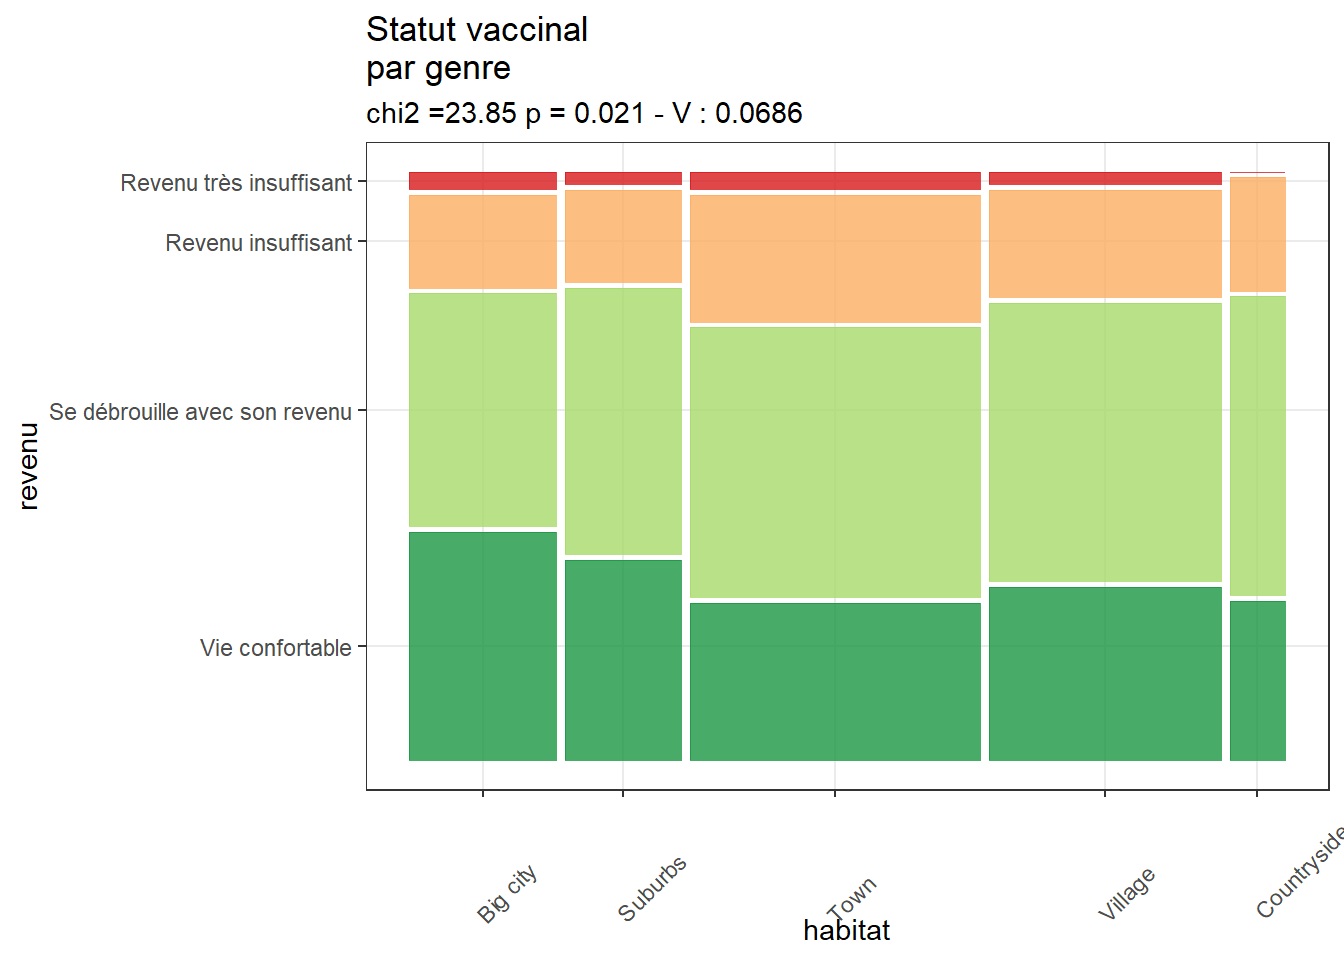
\includegraphics{bookdown-demo_files/figure-latex/327-1.pdf}

\hypertarget{les-chi2s-partiel-et-des-cartes-de-chaleur.}{%
\subsubsection{les chi2s partiel et des cartes de chaleur.}\label{les-chi2s-partiel-et-des-cartes-de-chaleur.}}

Une carte de chaleur représente une grandeur par un gradient de couleur pour chaque cellule définie par des variable x et y.

Faisons un premier essai pour représenter les effectifs, plutôt qu'avoir un tableau de nombres on va obtenir un tableau de couleurs.

L'arbre qui apparait en ligne et en colonne correspond au résultat d'une classification hiérarchiques que nous développons dans le chapitre X.

\begin{Shaded}
\begin{Highlighting}[]
\KeywordTok{library}\NormalTok{(pheatmap)}
\KeywordTok{library}\NormalTok{(viridis)}

\NormalTok{table2<-}\KeywordTok{as.data.frame}\NormalTok{(t) }\OperatorTok
\StringTok{  }\KeywordTok{pivot_wider}\NormalTok{(}\DataTypeTok{names_from =}\NormalTok{ Var1, }\DataTypeTok{values_from =}\NormalTok{ Freq) }\OperatorTok
\StringTok{  }\KeywordTok{column_to_rownames}\NormalTok{( }\DataTypeTok{var =} \StringTok{"Var2"}\NormalTok{)}
\KeywordTok{pheatmap}\NormalTok{(table2 , }\DataTypeTok{color =} \KeywordTok{rocket}\NormalTok{(}\DecValTok{10}\NormalTok{,}\DataTypeTok{direction =}\OperatorTok{-}\DecValTok{1}\NormalTok{))}
\end{Highlighting}
\end{Shaded}

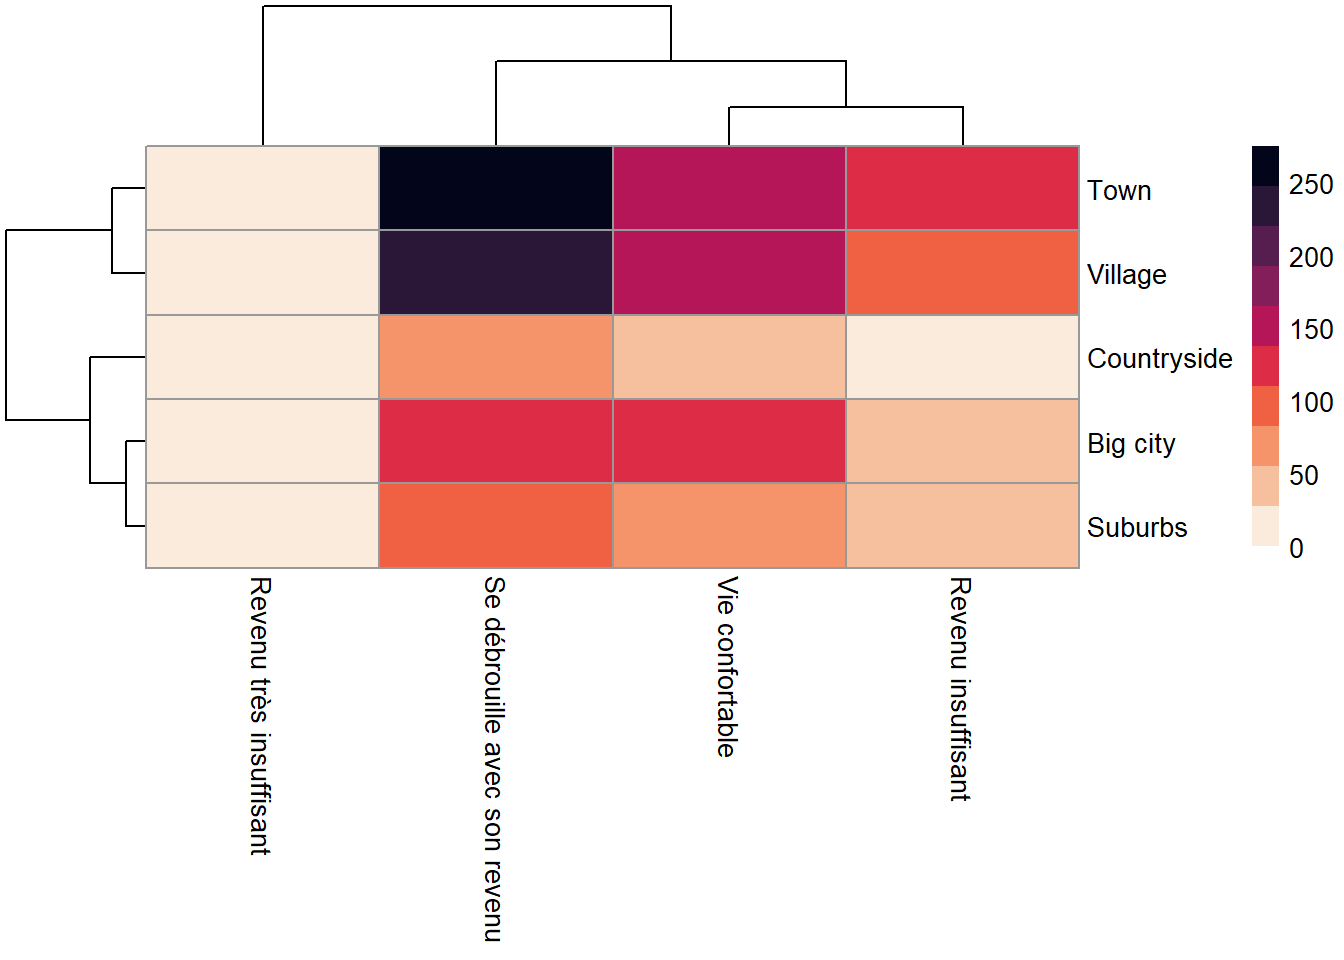
\includegraphics{bookdown-demo_files/figure-latex/328-1.pdf}

On utilise la même technique mais en représenant une grandeur différentes : les tests du chi2 partiels, pour apprécier les sous ou les sur-représentation.

\begin{Shaded}
\begin{Highlighting}[]
\KeywordTok{library}\NormalTok{(RColorBrewer)}
\NormalTok{chi2df<-}\StringTok{ }\KeywordTok{as.data.frame}\NormalTok{(chi2}\OperatorTok{$}\NormalTok{stdres)}

\NormalTok{table2<-chi2df }\OperatorTok\StringTok{ }
\StringTok{  }\KeywordTok{pivot_wider}\NormalTok{(}\DataTypeTok{names_from =}\NormalTok{ Var1, }\DataTypeTok{values_from =}\NormalTok{ Freq) }\OperatorTok
\StringTok{  }\KeywordTok{column_to_rownames}\NormalTok{( }\DataTypeTok{var =} \StringTok{"Var2"}\NormalTok{)}
\KeywordTok{pheatmap}\NormalTok{(table2 , }\DataTypeTok{color =} \KeywordTok{brewer.pal}\NormalTok{(}\DataTypeTok{n =} \DecValTok{9}\NormalTok{, }\DataTypeTok{name =} \StringTok{"RdBu"}\NormalTok{))}
\end{Highlighting}
\end{Shaded}

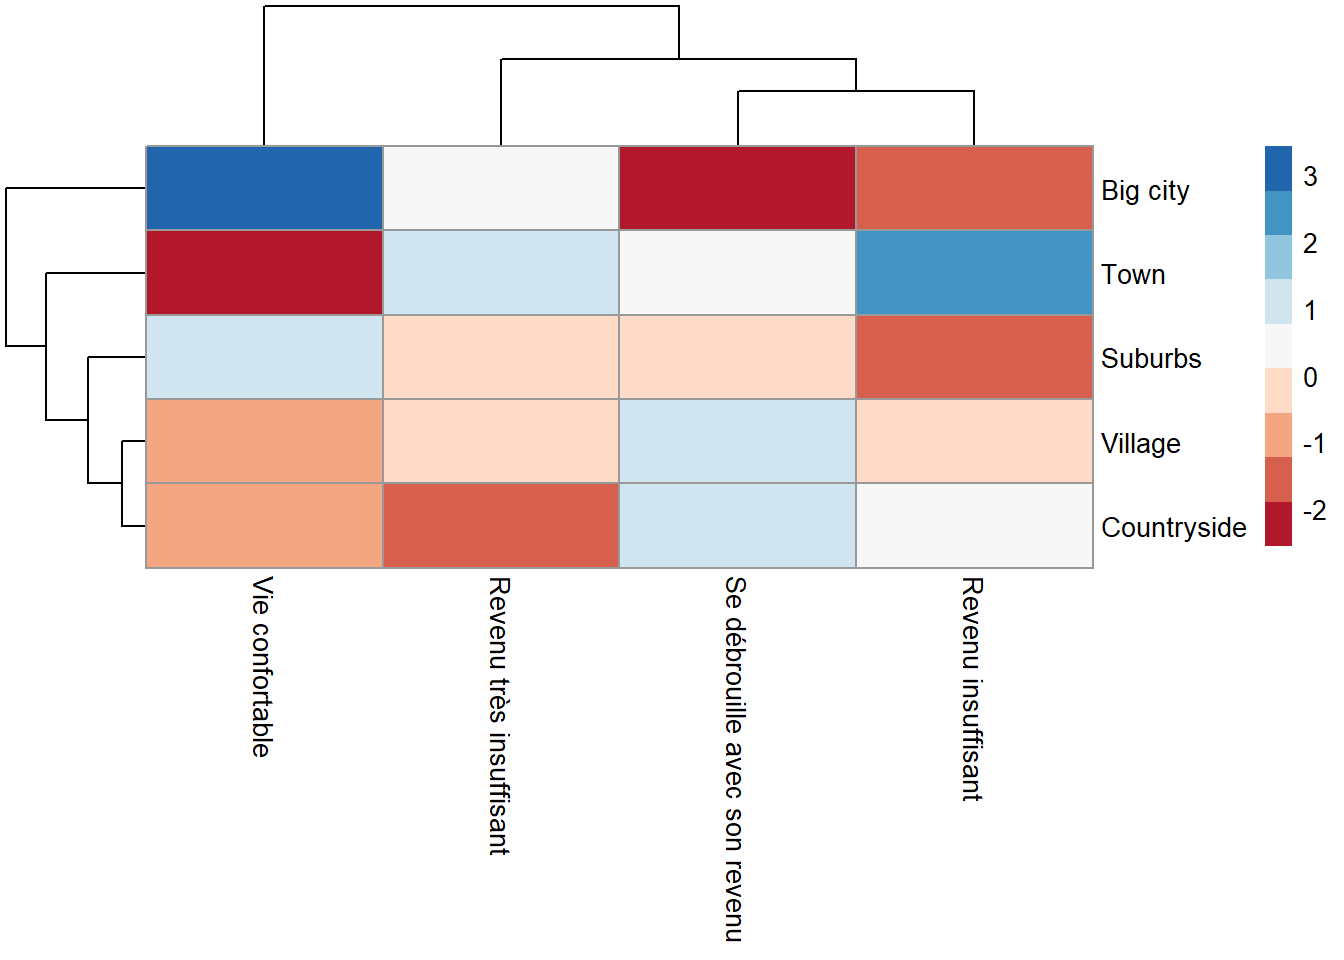
\includegraphics{bookdown-demo_files/figure-latex/329-1.pdf}

\hypertarget{les-treemaps-cest-merveilleux}{%
\subsubsection{Les treemaps, c'est merveilleux}\label{les-treemaps-cest-merveilleux}}

D'autre graphiques et des emboitements

\begin{Shaded}
\begin{Highlighting}[]
\KeywordTok{library}\NormalTok{(treemapify)}
\NormalTok{tree1<-df }\OperatorTok\StringTok{ }\KeywordTok{mutate}\NormalTok{(}\DataTypeTok{n=}\DecValTok{1}\NormalTok{)}\OperatorTok\KeywordTok{group_by}\NormalTok{(cntry,genre,habitat) }\OperatorTok\StringTok{ }\KeywordTok{summarize}\NormalTok{(}\DataTypeTok{n=}\KeywordTok{sum}\NormalTok{(n),}\DataTypeTok{mean=}\KeywordTok{mean}\NormalTok{(trust_interpersonnel, }\DataTypeTok{na.rm=}\OtherTok{TRUE}\NormalTok{))}

\NormalTok{g10 <-}\StringTok{ }\KeywordTok{ggplot}\NormalTok{(tree1, }\KeywordTok{aes}\NormalTok{(}\DataTypeTok{area =}\NormalTok{ n, }\DataTypeTok{fill=}\NormalTok{genre,}\DataTypeTok{subgroup=}\NormalTok{cntry)) }\OperatorTok{+}
\StringTok{  }\KeywordTok{geom_treemap}\NormalTok{() }\OperatorTok{+}\StringTok{   }
\StringTok{  }\KeywordTok{geom_treemap_text}\NormalTok{(}\KeywordTok{aes}\NormalTok{(}\DataTypeTok{label=}\NormalTok{habitat),}\DataTypeTok{colour =} \StringTok{"white"}\NormalTok{, }\DataTypeTok{place =} \StringTok{"centre"}\NormalTok{,}\DataTypeTok{grow =} \OtherTok{FALSE}\NormalTok{)}\OperatorTok{+}
\StringTok{      }\KeywordTok{geom_treemap_subgroup_text}\NormalTok{(}\DataTypeTok{color=}\StringTok{"white"}\NormalTok{,}\DataTypeTok{grow =} \OtherTok{FALSE}\NormalTok{)}\OperatorTok{+}
\StringTok{  }\KeywordTok{geom_treemap_subgroup_border}\NormalTok{()}
\NormalTok{g10}
\end{Highlighting}
\end{Shaded}

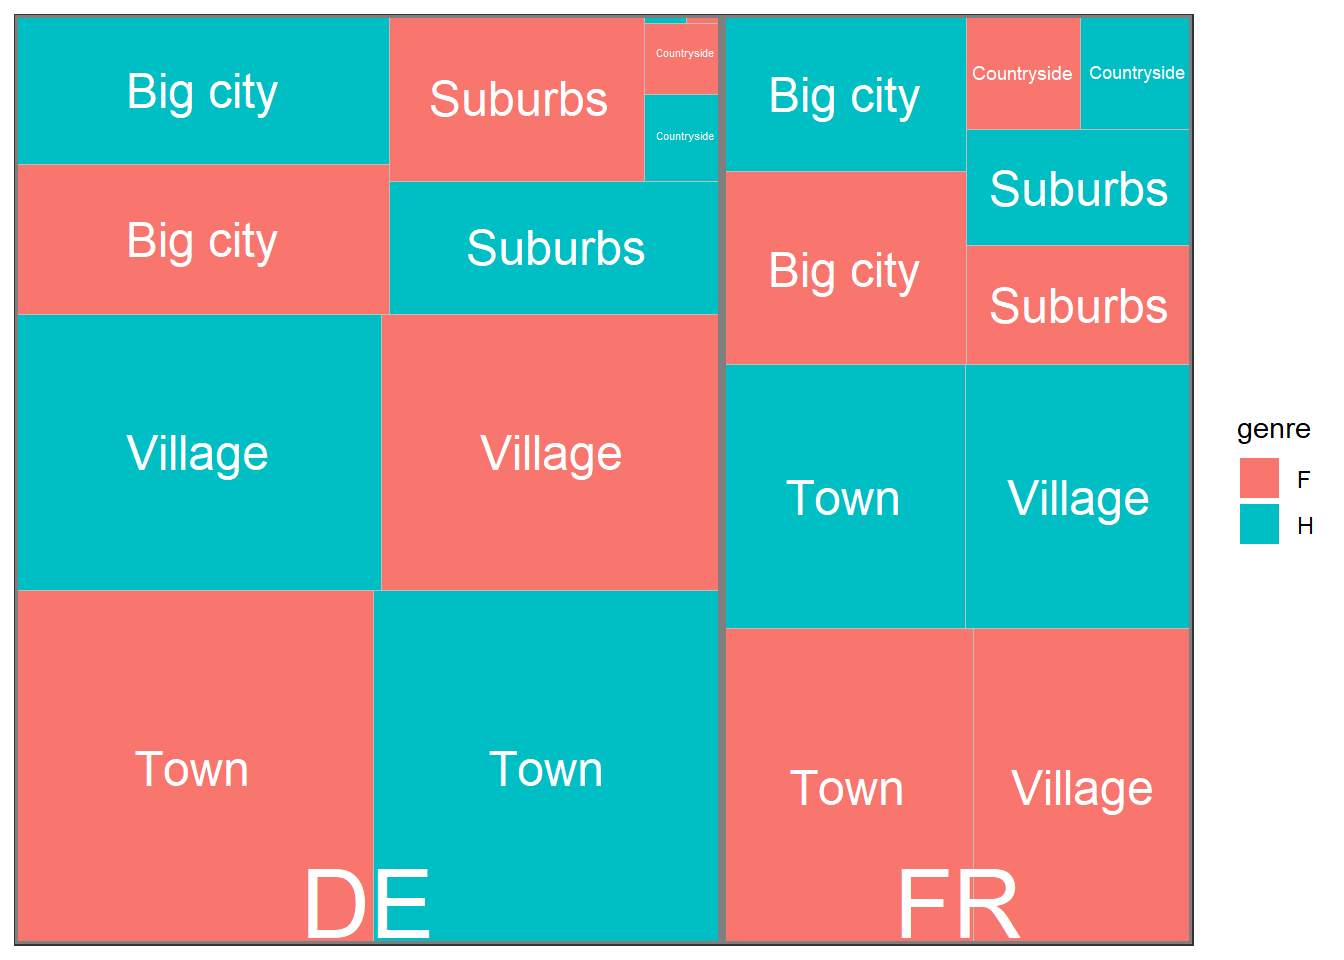
\includegraphics{bookdown-demo_files/figure-latex/330-1.pdf}

\hypertarget{analyse-graphique-multivariuxe9e}{%
\chapter{Analyse graphique multivariée}\label{analyse-graphique-multivariuxe9e}}

Dans ce chapitre, on généralise à des ensembles de variables.

\hypertarget{radar-plot}{%
\section{Radar plot}\label{radar-plot}}

\begin{Shaded}
\begin{Highlighting}[]
\NormalTok{rad<-df }\OperatorTok\StringTok{ }
\StringTok{  }\KeywordTok{group_by}\NormalTok{ (habitat,cntry) }\OperatorTok\StringTok{ }
\StringTok{  }\KeywordTok{summarize}\NormalTok{(}\DataTypeTok{Partis=}\KeywordTok{mean}\NormalTok{(Partis, }\DataTypeTok{na.rm=}\OtherTok{TRUE}\NormalTok{),}
  \DataTypeTok{Parlement=}\KeywordTok{mean}\NormalTok{(Parlement, }\DataTypeTok{na.rm=}\OtherTok{TRUE}\NormalTok{),}
  \DataTypeTok{Politiques=}\KeywordTok{mean}\NormalTok{(Politiques, }\DataTypeTok{na.rm=}\OtherTok{TRUE}\NormalTok{),}
  \DataTypeTok{Police=}\KeywordTok{mean}\NormalTok{(Police, }\DataTypeTok{na.rm=}\OtherTok{TRUE}\NormalTok{),}
  \DataTypeTok{Justice=}\KeywordTok{mean}\NormalTok{(Justice, }\DataTypeTok{na.rm=}\OtherTok{TRUE}\NormalTok{),}
  \DataTypeTok{NationsUnies=}\KeywordTok{mean}\NormalTok{(NationsUnies, }\DataTypeTok{na.rm=}\OtherTok{TRUE}\NormalTok{),}
  \DataTypeTok{ParlementEurop=}\KeywordTok{mean}\NormalTok{(ParlementEurop, }\DataTypeTok{na.rm=}\OtherTok{TRUE}\NormalTok{)) }\OperatorTok\StringTok{ }
\StringTok{  }\KeywordTok{filter}\NormalTok{(}\OperatorTok{!}\KeywordTok{is.na}\NormalTok{(habitat)) }\OperatorTok
\StringTok{  }\KeywordTok{gather}\NormalTok{(variable, value, }\OperatorTok{-}\NormalTok{habitat, }\OperatorTok{-}\NormalTok{cntry)}

\KeywordTok{ggplot}\NormalTok{(rad, }\KeywordTok{aes}\NormalTok{(}\DataTypeTok{x=}\KeywordTok{reorder}\NormalTok{(variable, value),}\DataTypeTok{y=}\NormalTok{value, }\DataTypeTok{group=}\NormalTok{habitat))}\OperatorTok{+}
\StringTok{  }\KeywordTok{geom_line}\NormalTok{(}\KeywordTok{aes}\NormalTok{(}\DataTypeTok{color=}\NormalTok{habitat), }\DataTypeTok{size=}\DecValTok{2}\NormalTok{)}\OperatorTok{+}
\StringTok{  }\KeywordTok{facet_grid}\NormalTok{(.}\OperatorTok{~}\NormalTok{cntry) }\OperatorTok{+}\KeywordTok{coord_flip}\NormalTok{()}\OperatorTok{+}
\StringTok{  }\KeywordTok{scale_color_brewer}\NormalTok{(}\DataTypeTok{type=}\StringTok{"div"}\NormalTok{,}\DataTypeTok{palette=}\DecValTok{3}\NormalTok{)}\OperatorTok{+}\KeywordTok{labs}\NormalTok{(}\DataTypeTok{title=} \StringTok{"Les éléments de la confiance institutionnelle"}\NormalTok{, }\DataTypeTok{caption=}\StringTok{"ESS2002-2018"}\NormalTok{,}\DataTypeTok{y=} \StringTok{"confiance (de 1 à 10)"}\NormalTok{,}\DataTypeTok{x=}\StringTok{"institutions"}\NormalTok{) }
\end{Highlighting}
\end{Shaded}

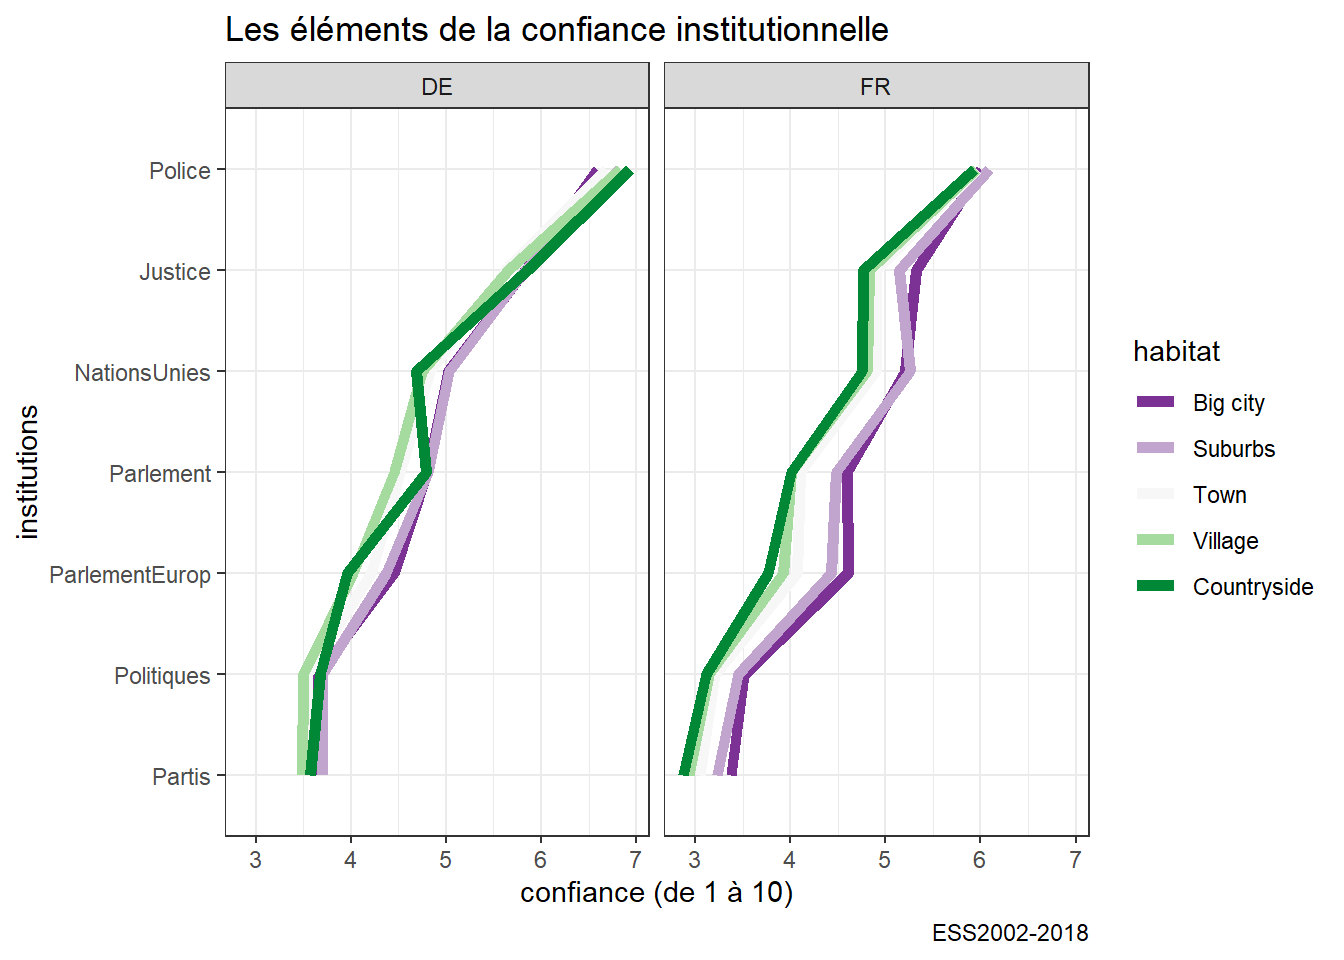
\includegraphics{bookdown-demo_files/figure-latex/430-1.pdf}

\begin{Shaded}
\begin{Highlighting}[]
\NormalTok{rad<-df }\OperatorTok\StringTok{ }
\StringTok{  }\KeywordTok{group_by}\NormalTok{ (Year,cntry) }\OperatorTok\StringTok{ }
\StringTok{  }\KeywordTok{summarize}\NormalTok{(}\DataTypeTok{Partis=}\KeywordTok{mean}\NormalTok{(Partis, }\DataTypeTok{na.rm=}\OtherTok{TRUE}\NormalTok{),}
  \DataTypeTok{Parlement=}\KeywordTok{mean}\NormalTok{(Parlement, }\DataTypeTok{na.rm=}\OtherTok{TRUE}\NormalTok{),}
  \DataTypeTok{Politiques=}\KeywordTok{mean}\NormalTok{(Politiques, }\DataTypeTok{na.rm=}\OtherTok{TRUE}\NormalTok{),}
  \DataTypeTok{Police=}\KeywordTok{mean}\NormalTok{(Police, }\DataTypeTok{na.rm=}\OtherTok{TRUE}\NormalTok{),}
  \DataTypeTok{Justice=}\KeywordTok{mean}\NormalTok{(Justice, }\DataTypeTok{na.rm=}\OtherTok{TRUE}\NormalTok{),}
  \DataTypeTok{NationsUnies=}\KeywordTok{mean}\NormalTok{(NationsUnies, }\DataTypeTok{na.rm=}\OtherTok{TRUE}\NormalTok{),}
  \DataTypeTok{ParlementEurop=}\KeywordTok{mean}\NormalTok{(ParlementEurop, }\DataTypeTok{na.rm=}\OtherTok{TRUE}\NormalTok{)) }\OperatorTok\StringTok{ }
\StringTok{  }\KeywordTok{gather}\NormalTok{(variable, value, }\OperatorTok{-}\NormalTok{Year, }\OperatorTok{-}\NormalTok{cntry)}

\KeywordTok{ggplot}\NormalTok{(rad, }\KeywordTok{aes}\NormalTok{(}\DataTypeTok{x=}\NormalTok{Year,}\DataTypeTok{y=}\NormalTok{value, }\DataTypeTok{group=}\NormalTok{variable))}\OperatorTok{+}
\StringTok{  }\KeywordTok{geom_line}\NormalTok{(}\KeywordTok{aes}\NormalTok{(}\DataTypeTok{color=}\NormalTok{variable), }\DataTypeTok{size=}\FloatTok{1.2}\NormalTok{)}\OperatorTok{+}
\StringTok{  }\KeywordTok{facet_wrap}\NormalTok{(.}\OperatorTok{~}\NormalTok{cntry, }\DataTypeTok{nrow=}\DecValTok{1}\NormalTok{) }\OperatorTok{+}
\StringTok{  }\KeywordTok{scale_color_brewer}\NormalTok{(}\DataTypeTok{palette=}\StringTok{"Spectral"}\NormalTok{)}\OperatorTok{+}\KeywordTok{labs}\NormalTok{(}\DataTypeTok{title=} \StringTok{"Les éléments de la confiance institutionnelle"}\NormalTok{, }\DataTypeTok{caption=}\StringTok{"ESS2002-2018"}\NormalTok{,}\DataTypeTok{y=} \StringTok{"confiance (de 1 à 10)"}\NormalTok{,}\DataTypeTok{x=}\StringTok{"institutions"}\NormalTok{) }
\end{Highlighting}
\end{Shaded}

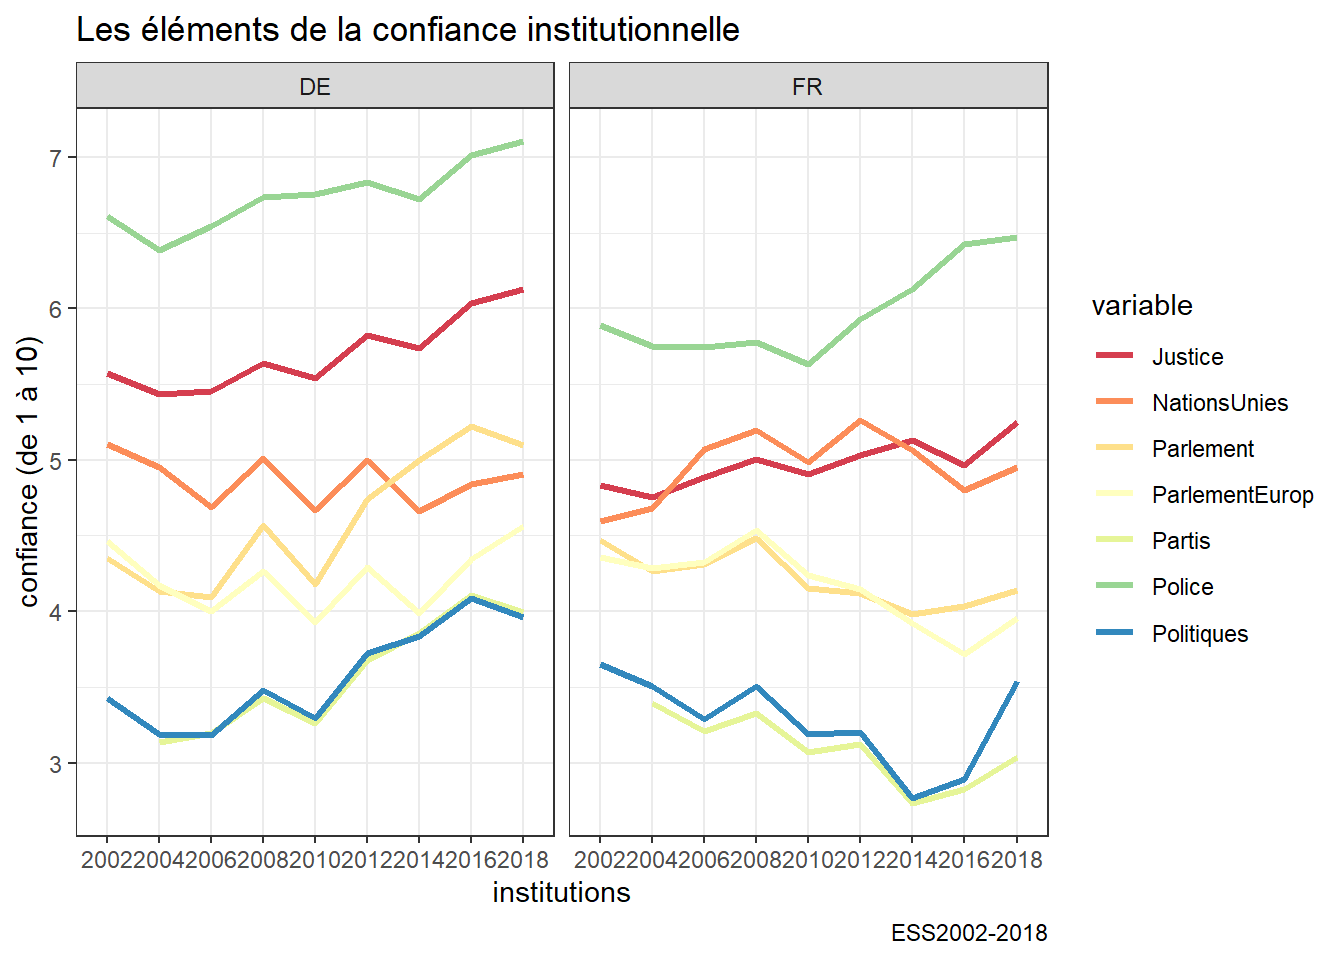
\includegraphics{bookdown-demo_files/figure-latex/431-1.pdf}

La différence entre les deux pays est claire, la rupture est accusée plus fortement en france qu'en allemagne. L'explication n'est sans doute pas culturelle mais démographique, un coup d'oeil à la carte des densité permet de comprendre mieux : \url{https://www.populationdata.net/cartes/allemagne-france-densite-de-population-2011/}.

\begin{Shaded}
\begin{Highlighting}[]
\KeywordTok{library}\NormalTok{(fmsb)}

\NormalTok{rad<-df }\OperatorTok\StringTok{ }\KeywordTok{filter}\NormalTok{(cntry}\OperatorTok{==}\StringTok{"FR"}\NormalTok{) }\OperatorTok
\StringTok{  }\KeywordTok{group_by}\NormalTok{ (habitat) }\OperatorTok
\StringTok{  }\KeywordTok{summarize}\NormalTok{(}\DataTypeTok{Partis=}\KeywordTok{mean}\NormalTok{(Partis, }\DataTypeTok{na.rm=}\OtherTok{TRUE}\NormalTok{),}
  \DataTypeTok{Parlement=}\KeywordTok{mean}\NormalTok{(Parlement, }\DataTypeTok{na.rm=}\OtherTok{TRUE}\NormalTok{),}
  \DataTypeTok{Politiques=}\KeywordTok{mean}\NormalTok{(Politiques, }\DataTypeTok{na.rm=}\OtherTok{TRUE}\NormalTok{),}
  \DataTypeTok{Police=}\KeywordTok{mean}\NormalTok{(Police, }\DataTypeTok{na.rm=}\OtherTok{TRUE}\NormalTok{),}
  \DataTypeTok{Justice=}\KeywordTok{mean}\NormalTok{(Justice, }\DataTypeTok{na.rm=}\OtherTok{TRUE}\NormalTok{),}
  \DataTypeTok{NationsUnies=}\KeywordTok{mean}\NormalTok{(NationsUnies, }\DataTypeTok{na.rm=}\OtherTok{TRUE}\NormalTok{),}
  \DataTypeTok{ParlementEurop=}\KeywordTok{mean}\NormalTok{(ParlementEurop, }\DataTypeTok{na.rm=}\OtherTok{TRUE}\NormalTok{)) }\OperatorTok\StringTok{ }\KeywordTok{filter}\NormalTok{(}\OperatorTok{!}\KeywordTok{is.na}\NormalTok{(habitat)) }\OperatorTok\StringTok{ }\NormalTok{dplyr}\OperatorTok{::}\KeywordTok{select}\NormalTok{(}\OperatorTok{-}\NormalTok{habitat)}

\CommentTok{#on doit indiquer les valeurs minimale et maximale - la fonction rep permet de repeter (ici 7 fois pour les 7 variables/col)}
\NormalTok{data <-}\StringTok{ }\KeywordTok{rbind}\NormalTok{(}\KeywordTok{rep}\NormalTok{(}\DecValTok{7}\NormalTok{,}\DecValTok{7}\NormalTok{) , }\KeywordTok{rep}\NormalTok{(}\DecValTok{3}\NormalTok{,}\DecValTok{7}\NormalTok{) , rad)}
\CommentTok{#l'autre method c'est ce choisir maxmin=FALSE}

\KeywordTok{rownames}\NormalTok{(rad) <-}\StringTok{ }\KeywordTok{c}\NormalTok{(}\StringTok{"big city"}\NormalTok{, }\StringTok{"suburbs"}\NormalTok{ ,}\StringTok{"town"}\NormalTok{,}\StringTok{"village"}\NormalTok{, }\StringTok{"countryside"}\NormalTok{)}
\KeywordTok{radarchart}\NormalTok{(rad, }\DataTypeTok{axistype=}\DecValTok{0}\NormalTok{, }\DataTypeTok{seg=}\DecValTok{4}\NormalTok{, }\DataTypeTok{title=}\StringTok{"Moyenne par institution"}\NormalTok{, }\DataTypeTok{maxmin=}\OtherTok{FALSE}\NormalTok{)}
\KeywordTok{legend}\NormalTok{(}\DataTypeTok{x=}\FloatTok{0.7}\NormalTok{, }\DataTypeTok{y=}\DecValTok{1}\NormalTok{, }\DataTypeTok{legend =} \KeywordTok{rownames}\NormalTok{(rad), }\DataTypeTok{bty =} \StringTok{"n"}\NormalTok{,}\DataTypeTok{text.col =} \StringTok{"grey"}\NormalTok{, }\DataTypeTok{cex=}\FloatTok{1.2}\NormalTok{, }\DataTypeTok{pt.cex=}\DecValTok{3}\NormalTok{)}
\end{Highlighting}
\end{Shaded}

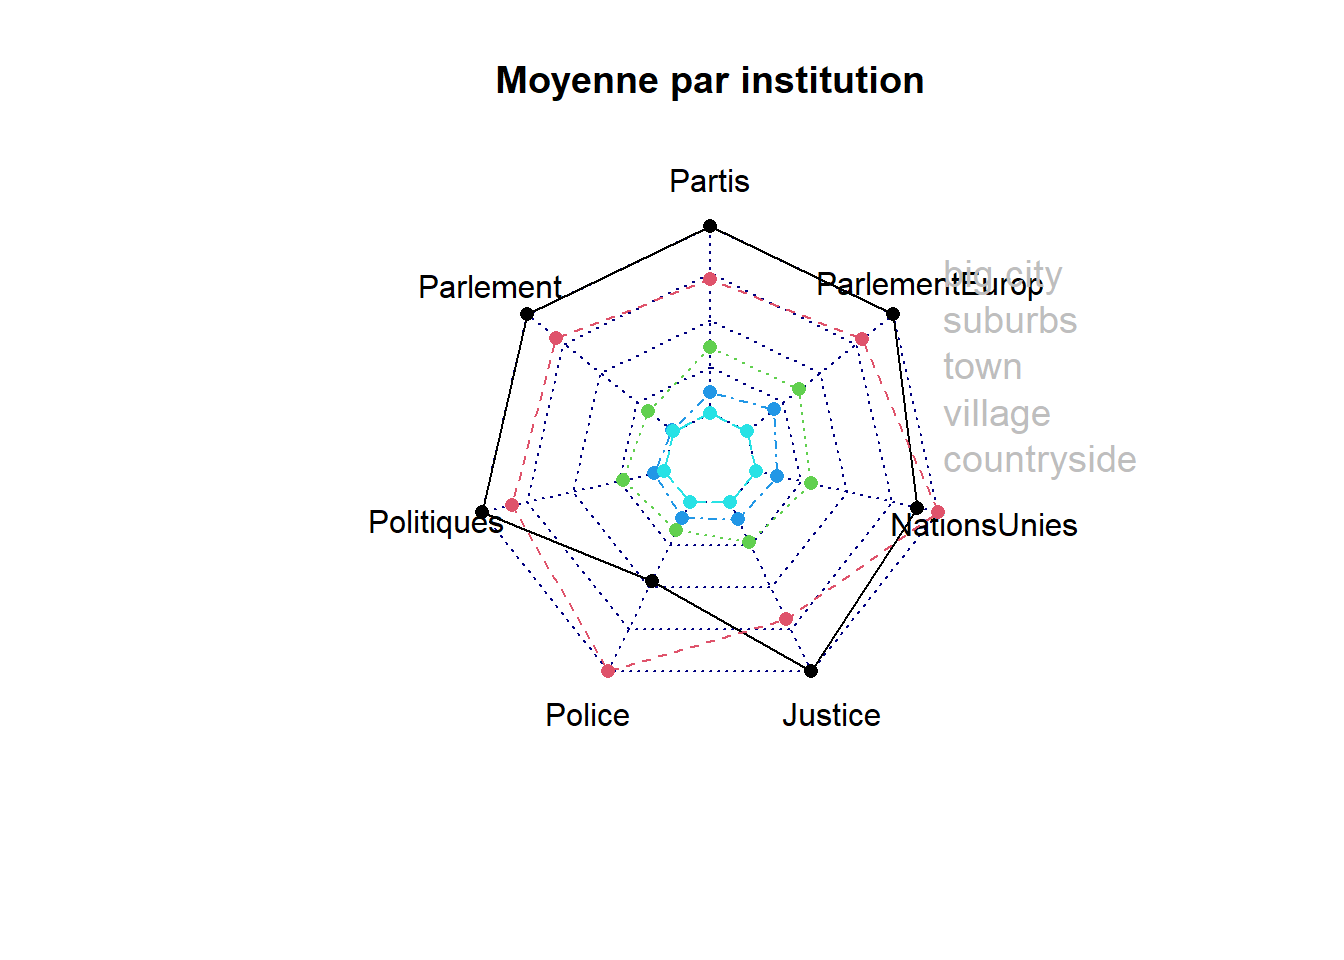
\includegraphics{bookdown-demo_files/figure-latex/432-1.pdf}

\hypertarget{tableau-de-corruxe9lation}{%
\section{Tableau de corrélation}\label{tableau-de-corruxe9lation}}

\hypertarget{facettes-qq-quanti}{%
\section{facettes( qq quanti)}\label{facettes-qq-quanti}}

\hypertarget{cowplot}{%
\section{cowplot}\label{cowplot}}

\hypertarget{LM}{%
\chapter{Modèles linéaire}\label{LM}}

voir \href{https://github.com/BenaventC/Covoiturage}{blablacar}

\hypertarget{FA}{%
\chapter{Analyse factorielle}\label{FA}}

l'objectif des méthodes d'analyses factorielles est de réduire un ensemble de variables à un petit nombre de dimensions qui résument l'essentiel de l'information.

\hypertarget{un-peu-de-thuxe9orie}{%
\section{Un peu de théorie}\label{un-peu-de-thuxe9orie}}

deux grandes approches marquent le paysage

la première est celle de l'ACP

La seconde est celle des psychologues et en particulier le modèle en terme de facteurs communs et spécifiques.

\hypertarget{application}{%
\section{Application}\label{application}}

\begin{Shaded}
\begin{Highlighting}[]
\KeywordTok{library}\NormalTok{(readr)}
\NormalTok{df <-}\StringTok{ }\KeywordTok{read_csv}\NormalTok{(}\StringTok{"./Data/ESS1-9e01_1.csv"}\NormalTok{)}
\KeywordTok{ls}\NormalTok{(df)}
\end{Highlighting}
\end{Shaded}

\begin{verbatim}
##   [1] "actrolg"  "aesfdrk"  "agea"     "anctry1"  "anweight" "atchctr" 
##   [7] "atcherp"  "badge"    "bctprd"   "brghmef"  "brghmwr"  "brncntr" 
##  [13] "cedition" "chldhm"   "cmsrv"    "cname"    "cntbrth"  "cntry"   
##  [19] "contplt"  "cproddat" "cptppol"  "cregion"  "crmvct"   "crvctef" 
##  [25] "crvctwr"  "cseqno"   "dsbld"    "dweight"  "edctn"    "edition" 
##  [31] "edulvlb"  "eduyrs"   "eisced"   "essround" "estsz"    "euftf"   
##  [37] "freehms"  "gincdif"  "gndr"     "gndr2"    "happy"    "health"  
##  [43] "hhmmb"    "hincfel"  "hinctnta" "hlthhmp"  "hmsacld"  "hmsfmlsh"
##  [49] "hswrk"    "idno"     "imbgeco"  "imdfetn"  "impcntr"  "impdiff" 
##  [55] "impenv"   "impfree"  "impfun"   "imprich"  "impsafe"  "imptrad" 
##  [61] "imsmetn"  "imueclt"  "imwbcnt"  "inmdisc"  "inprdsc"  "iorgact" 
##  [67] "ipadvnt"  "ipbhprp"  "ipcrtiv"  "ipeqopt"  "ipfrule"  "ipgdtim" 
##  [73] "iphlppl"  "iplylfr"  "ipmodst"  "iprspot"  "ipshabt"  "ipstrgv" 
##  [79] "ipsuces"  "ipudrst"  "jbspv"    "lrscale"  "maritalb" "nacer1"  
##  [85] "name"     "netuse"   "netusoft" "netustm"  "njbspv"   "nwspol"  
##  [91] "nwsppol"  "nwsptot"  "partner"  "pbldmn"   "pdwrk"    "polcmpl" 
##  [97] "polintr"  "pplfair"  "pplhlp"   "ppltrst"  "pray"     "prtyban" 
## [103] "psppipl"  "psppsgv"  "pspwght"  "pstplonl" "pweight"  "rdpol"   
## [109] "rdtot"    "regunit"  "rlgatnd"  "rlgblg"   "rlgdgr"   "rlgdnm"  
## [115] "rshpsts"  "rtrd"     "sclact"   "sclmeet"  "scnsenv"  "sgnptit" 
## [121] "stfdem"   "stfeco"   "stfedu"   "stfgov"   "stfhlth"  "stflife" 
## [127] "tporgwk"  "trstep"   "trstlgl"  "trstplc"  "trstplt"  "trstprl" 
## [133] "trstprt"  "trstun"   "tvpol"    "tvtot"    "uempla"   "uempli"  
## [139] "vote"     "wrkorg"   "wrkprty"  "yrbrn"
\end{verbatim}

valeur de kahle

IPCRTIV Important to think new ideas and being creative
IMPRICH Important to be rich, have money and expensive things
IPEQOPT Important that people are treated equally and have equal opportunities
IPSHABT Important to show abilities and be admired
IMPSAFE Important to live in secure and safe surroundings
IMPDIFF Important to try new and different things in life
IPFRULE Important to do what is told and follow rules
IPUDRST Important to understand different people
IPMODST Important to be humble and modest, not draw attention
IPGDTIM Important to have a good time
IMPFREE Important to make own decisions and be free
IPHLPPL Important to help people and care for others well-being
IPSUCES Important to be successful and that people recognise achievements
IPSTRGV Important that government is strong and ensures safety
IPADVNT Important to seek adventures and have an exciting life
IPBHPRP Important to behave properly
IPRSPOT Important to get respect from others
IPLYLFR Important to be loyal to friends and devote to people close
IMPENV Important to care for nature and environment
IMPTRAD Important to follow traditions and customs
IMPFUN Important to seek fun and things that give pleasure

()

\begin{Shaded}
\begin{Highlighting}[]
\KeywordTok{library}\NormalTok{(tidyverse)}


\NormalTok{foo<-df }\OperatorTok\StringTok{ }
\StringTok{  }\NormalTok{dplyr}\OperatorTok{::}\KeywordTok{select}\NormalTok{(ipcrtiv,}
\NormalTok{         imprich, }
\NormalTok{         ipeqopt, }
\NormalTok{         ipshabt, }
\NormalTok{         impsafe, }
\NormalTok{         impdiff, }
\NormalTok{         ipfrule, }
\NormalTok{         ipudrst, }
\NormalTok{         ipmodst, ipgdtim, impfree, iphlppl, ipsuces,ipstrgv, ipadvnt,ipbhprp,iprspot,iplylfr,impenv,imptrad, impfun)}

\KeywordTok{library}\NormalTok{(psych)}

\NormalTok{fa <-}\StringTok{ }\KeywordTok{fa}\NormalTok{(foo,}\DecValTok{4}\NormalTok{,}\DataTypeTok{fm=}\StringTok{"pa"}\NormalTok{ ,}\DataTypeTok{rotate=}\StringTok{"promax"}\NormalTok{)  }\CommentTok{#principal axis }
\NormalTok{fa}
\end{Highlighting}
\end{Shaded}

\begin{verbatim}
## Factor Analysis using method =  pa
## Call: fa(r = foo, nfactors = 4, rotate = "promax", fm = "pa")
## Standardized loadings (pattern matrix) based upon correlation matrix
##           PA1   PA3   PA2   PA4   h2   u2 com
## ipcrtiv  0.63 -0.18  0.28 -0.01 0.48 0.52 1.5
## imprich -0.12  0.07  0.62  0.08 0.42 0.58 1.1
## ipeqopt  0.74  0.11  0.01 -0.14 0.55 0.45 1.1
## ipshabt  0.17  0.03  0.74 -0.13 0.59 0.41 1.2
## impsafe  0.18  0.56  0.18 -0.16 0.51 0.49 1.6
## impdiff  0.40 -0.15  0.25  0.28 0.53 0.47 2.8
## ipfrule -0.01  0.58  0.15 -0.10 0.38 0.62 1.2
## ipudrst  0.77  0.09 -0.05 -0.05 0.59 0.41 1.0
## ipmodst  0.36  0.47 -0.16 -0.03 0.44 0.56 2.2
## ipgdtim  0.12  0.01  0.13  0.52 0.49 0.51 1.2
## impfree  0.48  0.05  0.12  0.16 0.51 0.49 1.4
## iphlppl  0.58  0.27 -0.09  0.07 0.62 0.38 1.5
## ipsuces  0.00  0.11  0.66  0.09 0.60 0.40 1.1
## ipstrgv  0.11  0.55  0.07  0.05 0.48 0.52 1.1
## ipadvnt  0.08 -0.22  0.31  0.50 0.53 0.47 2.2
## ipbhprp -0.01  0.75  0.02  0.01 0.57 0.43 1.0
## iprspot -0.15  0.44  0.43  0.06 0.46 0.54 2.3
## iplylfr  0.45  0.34 -0.10  0.20 0.62 0.38 2.4
## impenv   0.48  0.34 -0.13  0.11 0.56 0.44 2.1
## imptrad -0.07  0.69 -0.05  0.12 0.45 0.55 1.1
## impfun  -0.10  0.11 -0.02  0.84 0.65 0.35 1.1
## 
##                        PA1  PA3  PA2  PA4
## SS loadings           3.57 3.40 2.28 1.78
## Proportion Var        0.17 0.16 0.11 0.08
## Cumulative Var        0.17 0.33 0.44 0.53
## Proportion Explained  0.32 0.31 0.21 0.16
## Cumulative Proportion 0.32 0.63 0.84 1.00
## 
##  With factor correlations of 
##      PA1  PA3  PA2  PA4
## PA1 1.00 0.64 0.52 0.68
## PA3 0.64 1.00 0.43 0.37
## PA2 0.52 0.43 1.00 0.65
## PA4 0.68 0.37 0.65 1.00
## 
## Mean item complexity =  1.5
## Test of the hypothesis that 4 factors are sufficient.
## 
## The degrees of freedom for the null model are  210  and the objective function was  10.13 with Chi Square of  2591740
## The degrees of freedom for the model are 132  and the objective function was  0.3 
## 
## The root mean square of the residuals (RMSR) is  0.02 
## The df corrected root mean square of the residuals is  0.02 
## 
## The harmonic number of observations is  252609 with the empirical chi square  36298.97  with prob <  0 
## The total number of observations was  255824  with Likelihood Chi Square =  76645.06  with prob <  0 
## 
## Tucker Lewis Index of factoring reliability =  0.953
## RMSEA index =  0.048  and the 90 % confidence intervals are  0.047 0.048
## BIC =  75001.36
## Fit based upon off diagonal values = 1
## Measures of factor score adequacy             
##                                                    PA1  PA3  PA2  PA4
## Correlation of (regression) scores with factors   0.94 0.93 0.91 0.91
## Multiple R square of scores with factors          0.89 0.87 0.83 0.83
## Minimum correlation of possible factor scores     0.78 0.73 0.67 0.66
\end{verbatim}

\begin{Shaded}
\begin{Highlighting}[]
\KeywordTok{library}\NormalTok{(flextable)}

\CommentTok{#une fonction utile}


\NormalTok{flex <-}\StringTok{ }\ControlFlowTok{function}\NormalTok{(data, }\DataTypeTok{title=}\OtherTok{NULL}\NormalTok{) \{}
  \CommentTok{# this grabs the data and converts it to a flextbale}
  \KeywordTok{flextable}\NormalTok{(data) }\OperatorTok
\StringTok{  }\CommentTok{# this makes the table fill the page width}
\StringTok{  }\KeywordTok{set_table_properties}\NormalTok{(}\DataTypeTok{layout =} \StringTok{"autofit"}\NormalTok{, }\DataTypeTok{width =} \DecValTok{1}\NormalTok{) }\OperatorTok
\StringTok{  }\CommentTok{# font size}
\StringTok{  }\KeywordTok{fontsize}\NormalTok{(}\DataTypeTok{size=}\DecValTok{10}\NormalTok{, }\DataTypeTok{part=}\StringTok{"all"}\NormalTok{) }\OperatorTok
\StringTok{    }\CommentTok{#this adds a ttitlecreates an automatic table number}
\StringTok{      }\KeywordTok{set_caption}\NormalTok{(title, }
                  \DataTypeTok{autonum =}\NormalTok{ officer}\OperatorTok{::}\KeywordTok{run_autonum}\NormalTok{(}\DataTypeTok{seq_id =} \StringTok{"tab"}\NormalTok{, }
                                                 \DataTypeTok{pre_label =} \StringTok{"Table "}\NormalTok{, }
                                                 \DataTypeTok{post_label =} \StringTok{"}\CharTok{\textbackslash{}n}\StringTok{"}\NormalTok{, }
                                                 \DataTypeTok{bkm =} \StringTok{"anytable"}\NormalTok{)) }\OperatorTok
\StringTok{  }\CommentTok{# font type}
\StringTok{  }\KeywordTok{font}\NormalTok{(}\DataTypeTok{fontname=}\StringTok{"Times New Roman"}\NormalTok{, }\DataTypeTok{part=}\StringTok{"all"}\NormalTok{)}
\NormalTok{\}}

\NormalTok{fa[[}\StringTok{"Vaccounted"}\NormalTok{]] }\OperatorTok
\StringTok{  }\KeywordTok{as.data.frame}\NormalTok{() }\OperatorTok
\StringTok{  }\CommentTok{#select(1:5) %>% Use this if you have many factors and only want to show a certain number}
\StringTok{  }\KeywordTok{rownames_to_column}\NormalTok{(}\StringTok{"Property"}\NormalTok{) }\OperatorTok
\StringTok{    }\KeywordTok{mutate}\NormalTok{(}\KeywordTok{across}\NormalTok{(}\KeywordTok{where}\NormalTok{(is.numeric), round, }\DecValTok{3}\NormalTok{)) }\OperatorTok
\StringTok{    }\KeywordTok{flex}\NormalTok{(}\StringTok{"Eigenvalues and Variance Explained for Rotated Factor Solution"}\NormalTok{)}
\end{Highlighting}
\end{Shaded}

\providecommand{\docline}[3]{\noalign{\global\setlength{\arrayrulewidth}{#1}}\arrayrulecolor[HTML]{#2}\cline{#3}}

\setlength{\tabcolsep}{2pt}

\renewcommand*{\arraystretch}{1.5}

\begin{longtable}[c]{ccccc}

\caption{Eigenvalues and Variance Explained for Rotated Factor Solution}\label{tab:anytable}\\

\hhline{>{\arrayrulecolor[HTML]{666666}\global\arrayrulewidth=2pt}->{\arrayrulecolor[HTML]{666666}\global\arrayrulewidth=2pt}->{\arrayrulecolor[HTML]{666666}\global\arrayrulewidth=2pt}->{\arrayrulecolor[HTML]{666666}\global\arrayrulewidth=2pt}->{\arrayrulecolor[HTML]{666666}\global\arrayrulewidth=2pt}-}

\multicolumn{1}{!{\color[HTML]{000000}\vrule width 0pt}>{}l}{\fontsize{10}{10}\selectfont{\textcolor[HTML]{000000}{\global\setmainfont{Times New Roman}{Property}}}} & \multicolumn{1}{!{\color[HTML]{000000}\vrule width 0pt}>{}r}{\fontsize{10}{10}\selectfont{\textcolor[HTML]{000000}{\global\setmainfont{Times New Roman}{PA1}}}} & \multicolumn{1}{!{\color[HTML]{000000}\vrule width 0pt}>{}r}{\fontsize{10}{10}\selectfont{\textcolor[HTML]{000000}{\global\setmainfont{Times New Roman}{PA3}}}} & \multicolumn{1}{!{\color[HTML]{000000}\vrule width 0pt}>{}r}{\fontsize{10}{10}\selectfont{\textcolor[HTML]{000000}{\global\setmainfont{Times New Roman}{PA2}}}} & \multicolumn{1}{!{\color[HTML]{000000}\vrule width 0pt}>{}r!{\color[HTML]{000000}\vrule width 0pt}}{\fontsize{10}{10}\selectfont{\textcolor[HTML]{000000}{\global\setmainfont{Times New Roman}{PA4}}}} \\

\noalign{\global\setlength{\arrayrulewidth}{2pt}}\arrayrulecolor[HTML]{666666}\cline{1-5}

\endfirsthead

\hhline{>{\arrayrulecolor[HTML]{666666}\global\arrayrulewidth=2pt}->{\arrayrulecolor[HTML]{666666}\global\arrayrulewidth=2pt}->{\arrayrulecolor[HTML]{666666}\global\arrayrulewidth=2pt}->{\arrayrulecolor[HTML]{666666}\global\arrayrulewidth=2pt}->{\arrayrulecolor[HTML]{666666}\global\arrayrulewidth=2pt}-}

\multicolumn{1}{!{\color[HTML]{000000}\vrule width 0pt}>{}l}{\fontsize{10}{10}\selectfont{\textcolor[HTML]{000000}{\global\setmainfont{Times New Roman}{Property}}}} & \multicolumn{1}{!{\color[HTML]{000000}\vrule width 0pt}>{}r}{\fontsize{10}{10}\selectfont{\textcolor[HTML]{000000}{\global\setmainfont{Times New Roman}{PA1}}}} & \multicolumn{1}{!{\color[HTML]{000000}\vrule width 0pt}>{}r}{\fontsize{10}{10}\selectfont{\textcolor[HTML]{000000}{\global\setmainfont{Times New Roman}{PA3}}}} & \multicolumn{1}{!{\color[HTML]{000000}\vrule width 0pt}>{}r}{\fontsize{10}{10}\selectfont{\textcolor[HTML]{000000}{\global\setmainfont{Times New Roman}{PA2}}}} & \multicolumn{1}{!{\color[HTML]{000000}\vrule width 0pt}>{}r!{\color[HTML]{000000}\vrule width 0pt}}{\fontsize{10}{10}\selectfont{\textcolor[HTML]{000000}{\global\setmainfont{Times New Roman}{PA4}}}} \\

\noalign{\global\setlength{\arrayrulewidth}{2pt}}\arrayrulecolor[HTML]{666666}\cline{1-5}\endhead



\multicolumn{1}{!{\color[HTML]{000000}\vrule width 0pt}>{}l}{\fontsize{10}{10}\selectfont{\textcolor[HTML]{000000}{\global\setmainfont{Times New Roman}{SS\ loadings}}}} & \multicolumn{1}{!{\color[HTML]{000000}\vrule width 0pt}>{}r}{\fontsize{10}{10}\selectfont{\textcolor[HTML]{000000}{\global\setmainfont{Times New Roman}{3.573}}}} & \multicolumn{1}{!{\color[HTML]{000000}\vrule width 0pt}>{}r}{\fontsize{10}{10}\selectfont{\textcolor[HTML]{000000}{\global\setmainfont{Times New Roman}{3.404}}}} & \multicolumn{1}{!{\color[HTML]{000000}\vrule width 0pt}>{}r}{\fontsize{10}{10}\selectfont{\textcolor[HTML]{000000}{\global\setmainfont{Times New Roman}{2.282}}}} & \multicolumn{1}{!{\color[HTML]{000000}\vrule width 0pt}>{}r!{\color[HTML]{000000}\vrule width 0pt}}{\fontsize{10}{10}\selectfont{\textcolor[HTML]{000000}{\global\setmainfont{Times New Roman}{1.782}}}} \\





\multicolumn{1}{!{\color[HTML]{000000}\vrule width 0pt}>{}l}{\fontsize{10}{10}\selectfont{\textcolor[HTML]{000000}{\global\setmainfont{Times New Roman}{Proportion\ Var}}}} & \multicolumn{1}{!{\color[HTML]{000000}\vrule width 0pt}>{}r}{\fontsize{10}{10}\selectfont{\textcolor[HTML]{000000}{\global\setmainfont{Times New Roman}{0.170}}}} & \multicolumn{1}{!{\color[HTML]{000000}\vrule width 0pt}>{}r}{\fontsize{10}{10}\selectfont{\textcolor[HTML]{000000}{\global\setmainfont{Times New Roman}{0.162}}}} & \multicolumn{1}{!{\color[HTML]{000000}\vrule width 0pt}>{}r}{\fontsize{10}{10}\selectfont{\textcolor[HTML]{000000}{\global\setmainfont{Times New Roman}{0.109}}}} & \multicolumn{1}{!{\color[HTML]{000000}\vrule width 0pt}>{}r!{\color[HTML]{000000}\vrule width 0pt}}{\fontsize{10}{10}\selectfont{\textcolor[HTML]{000000}{\global\setmainfont{Times New Roman}{0.085}}}} \\





\multicolumn{1}{!{\color[HTML]{000000}\vrule width 0pt}>{}l}{\fontsize{10}{10}\selectfont{\textcolor[HTML]{000000}{\global\setmainfont{Times New Roman}{Cumulative\ Var}}}} & \multicolumn{1}{!{\color[HTML]{000000}\vrule width 0pt}>{}r}{\fontsize{10}{10}\selectfont{\textcolor[HTML]{000000}{\global\setmainfont{Times New Roman}{0.170}}}} & \multicolumn{1}{!{\color[HTML]{000000}\vrule width 0pt}>{}r}{\fontsize{10}{10}\selectfont{\textcolor[HTML]{000000}{\global\setmainfont{Times New Roman}{0.332}}}} & \multicolumn{1}{!{\color[HTML]{000000}\vrule width 0pt}>{}r}{\fontsize{10}{10}\selectfont{\textcolor[HTML]{000000}{\global\setmainfont{Times New Roman}{0.441}}}} & \multicolumn{1}{!{\color[HTML]{000000}\vrule width 0pt}>{}r!{\color[HTML]{000000}\vrule width 0pt}}{\fontsize{10}{10}\selectfont{\textcolor[HTML]{000000}{\global\setmainfont{Times New Roman}{0.526}}}} \\





\multicolumn{1}{!{\color[HTML]{000000}\vrule width 0pt}>{}l}{\fontsize{10}{10}\selectfont{\textcolor[HTML]{000000}{\global\setmainfont{Times New Roman}{Proportion\ Explained}}}} & \multicolumn{1}{!{\color[HTML]{000000}\vrule width 0pt}>{}r}{\fontsize{10}{10}\selectfont{\textcolor[HTML]{000000}{\global\setmainfont{Times New Roman}{0.324}}}} & \multicolumn{1}{!{\color[HTML]{000000}\vrule width 0pt}>{}r}{\fontsize{10}{10}\selectfont{\textcolor[HTML]{000000}{\global\setmainfont{Times New Roman}{0.308}}}} & \multicolumn{1}{!{\color[HTML]{000000}\vrule width 0pt}>{}r}{\fontsize{10}{10}\selectfont{\textcolor[HTML]{000000}{\global\setmainfont{Times New Roman}{0.207}}}} & \multicolumn{1}{!{\color[HTML]{000000}\vrule width 0pt}>{}r!{\color[HTML]{000000}\vrule width 0pt}}{\fontsize{10}{10}\selectfont{\textcolor[HTML]{000000}{\global\setmainfont{Times New Roman}{0.161}}}} \\





\multicolumn{1}{!{\color[HTML]{000000}\vrule width 0pt}>{}l}{\fontsize{10}{10}\selectfont{\textcolor[HTML]{000000}{\global\setmainfont{Times New Roman}{Cumulative\ Proportion}}}} & \multicolumn{1}{!{\color[HTML]{000000}\vrule width 0pt}>{}r}{\fontsize{10}{10}\selectfont{\textcolor[HTML]{000000}{\global\setmainfont{Times New Roman}{0.324}}}} & \multicolumn{1}{!{\color[HTML]{000000}\vrule width 0pt}>{}r}{\fontsize{10}{10}\selectfont{\textcolor[HTML]{000000}{\global\setmainfont{Times New Roman}{0.632}}}} & \multicolumn{1}{!{\color[HTML]{000000}\vrule width 0pt}>{}r}{\fontsize{10}{10}\selectfont{\textcolor[HTML]{000000}{\global\setmainfont{Times New Roman}{0.839}}}} & \multicolumn{1}{!{\color[HTML]{000000}\vrule width 0pt}>{}r!{\color[HTML]{000000}\vrule width 0pt}}{\fontsize{10}{10}\selectfont{\textcolor[HTML]{000000}{\global\setmainfont{Times New Roman}{1.000}}}} \\

\noalign{\global\setlength{\arrayrulewidth}{2pt}}\arrayrulecolor[HTML]{666666}\cline{1-5}



\end{longtable}

\begin{Shaded}
\begin{Highlighting}[]
\CommentTok{#et une seconde fonction}


\NormalTok{fa_table <-}\StringTok{ }\ControlFlowTok{function}\NormalTok{(x, cut) \{}
  \CommentTok{#get sorted loadings}
\NormalTok{  loadings <-}\StringTok{ }\KeywordTok{fa.sort}\NormalTok{(x)}\OperatorTok{$}\NormalTok{loadings }\OperatorTok\StringTok{ }\KeywordTok{round}\NormalTok{(}\DecValTok{3}\NormalTok{)}
  \CommentTok{#supress loadings}
\NormalTok{  loadings[loadings }\OperatorTok{<}\StringTok{ }\NormalTok{cut] <-}\StringTok{ ""}
  \CommentTok{#get additional info}
\NormalTok{  add_info <-}\StringTok{ }\KeywordTok{cbind}\NormalTok{(x}\OperatorTok{$}\NormalTok{communalities, }
\NormalTok{                    x}\OperatorTok{$}\NormalTok{uniquenesses,}
\NormalTok{                    x}\OperatorTok{$}\NormalTok{complexity) }\OperatorTok
\StringTok{    }\CommentTok{# make it a data frame}
\StringTok{    }\KeywordTok{as.data.frame}\NormalTok{() }\OperatorTok
\StringTok{    }\CommentTok{# column names}
\StringTok{    }\KeywordTok{rename}\NormalTok{(}\StringTok{"Communality"}\NormalTok{ =}\StringTok{ }\NormalTok{V1,}
           \StringTok{"Uniqueness"}\NormalTok{ =}\StringTok{ }\NormalTok{V2,}
           \StringTok{"Complexity"}\NormalTok{ =}\StringTok{ }\NormalTok{V3) }\OperatorTok
\StringTok{    }\CommentTok{#get the item names from the vector}
\StringTok{    }\KeywordTok{rownames_to_column}\NormalTok{(}\StringTok{"item"}\NormalTok{)}
  \CommentTok{#build table}
\NormalTok{  loadings }\OperatorTok
\StringTok{    }\KeywordTok{unclass}\NormalTok{() }\OperatorTok
\StringTok{    }\KeywordTok{as.data.frame}\NormalTok{() }\OperatorTok
\StringTok{    }\KeywordTok{rownames_to_column}\NormalTok{(}\StringTok{"item"}\NormalTok{) }\OperatorTok
\StringTok{    }\KeywordTok{left_join}\NormalTok{(add_info) }\OperatorTok
\StringTok{    }\KeywordTok{mutate}\NormalTok{(}\KeywordTok{across}\NormalTok{(}\KeywordTok{where}\NormalTok{(is.numeric), round, }\DecValTok{3}\NormalTok{))}
\NormalTok{\}}

\KeywordTok{fa_table}\NormalTok{(fa, }\FloatTok{.32}\NormalTok{)}\OperatorTok
\StringTok{  }\KeywordTok{flex}\NormalTok{(}\StringTok{"A Pretty Factor Analysis Table"}\NormalTok{)}
\end{Highlighting}
\end{Shaded}

\providecommand{\docline}[3]{\noalign{\global\setlength{\arrayrulewidth}{#1}}\arrayrulecolor[HTML]{#2}\cline{#3}}

\setlength{\tabcolsep}{2pt}

\renewcommand*{\arraystretch}{1.5}

\begin{longtable}[c]{cccccccc}

\caption{A Pretty Factor Analysis Table}\label{tab:anytable}\\

\hhline{>{\arrayrulecolor[HTML]{666666}\global\arrayrulewidth=2pt}->{\arrayrulecolor[HTML]{666666}\global\arrayrulewidth=2pt}->{\arrayrulecolor[HTML]{666666}\global\arrayrulewidth=2pt}->{\arrayrulecolor[HTML]{666666}\global\arrayrulewidth=2pt}->{\arrayrulecolor[HTML]{666666}\global\arrayrulewidth=2pt}->{\arrayrulecolor[HTML]{666666}\global\arrayrulewidth=2pt}->{\arrayrulecolor[HTML]{666666}\global\arrayrulewidth=2pt}->{\arrayrulecolor[HTML]{666666}\global\arrayrulewidth=2pt}-}

\multicolumn{1}{!{\color[HTML]{000000}\vrule width 0pt}>{}l}{\fontsize{10}{10}\selectfont{\textcolor[HTML]{000000}{\global\setmainfont{Times New Roman}{item}}}} & \multicolumn{1}{!{\color[HTML]{000000}\vrule width 0pt}>{}l}{\fontsize{10}{10}\selectfont{\textcolor[HTML]{000000}{\global\setmainfont{Times New Roman}{PA1}}}} & \multicolumn{1}{!{\color[HTML]{000000}\vrule width 0pt}>{}l}{\fontsize{10}{10}\selectfont{\textcolor[HTML]{000000}{\global\setmainfont{Times New Roman}{PA3}}}} & \multicolumn{1}{!{\color[HTML]{000000}\vrule width 0pt}>{}l}{\fontsize{10}{10}\selectfont{\textcolor[HTML]{000000}{\global\setmainfont{Times New Roman}{PA2}}}} & \multicolumn{1}{!{\color[HTML]{000000}\vrule width 0pt}>{}l}{\fontsize{10}{10}\selectfont{\textcolor[HTML]{000000}{\global\setmainfont{Times New Roman}{PA4}}}} & \multicolumn{1}{!{\color[HTML]{000000}\vrule width 0pt}>{}r}{\fontsize{10}{10}\selectfont{\textcolor[HTML]{000000}{\global\setmainfont{Times New Roman}{Communality}}}} & \multicolumn{1}{!{\color[HTML]{000000}\vrule width 0pt}>{}r}{\fontsize{10}{10}\selectfont{\textcolor[HTML]{000000}{\global\setmainfont{Times New Roman}{Uniqueness}}}} & \multicolumn{1}{!{\color[HTML]{000000}\vrule width 0pt}>{}r!{\color[HTML]{000000}\vrule width 0pt}}{\fontsize{10}{10}\selectfont{\textcolor[HTML]{000000}{\global\setmainfont{Times New Roman}{Complexity}}}} \\

\noalign{\global\setlength{\arrayrulewidth}{2pt}}\arrayrulecolor[HTML]{666666}\cline{1-8}

\endfirsthead

\hhline{>{\arrayrulecolor[HTML]{666666}\global\arrayrulewidth=2pt}->{\arrayrulecolor[HTML]{666666}\global\arrayrulewidth=2pt}->{\arrayrulecolor[HTML]{666666}\global\arrayrulewidth=2pt}->{\arrayrulecolor[HTML]{666666}\global\arrayrulewidth=2pt}->{\arrayrulecolor[HTML]{666666}\global\arrayrulewidth=2pt}->{\arrayrulecolor[HTML]{666666}\global\arrayrulewidth=2pt}->{\arrayrulecolor[HTML]{666666}\global\arrayrulewidth=2pt}->{\arrayrulecolor[HTML]{666666}\global\arrayrulewidth=2pt}-}

\multicolumn{1}{!{\color[HTML]{000000}\vrule width 0pt}>{}l}{\fontsize{10}{10}\selectfont{\textcolor[HTML]{000000}{\global\setmainfont{Times New Roman}{item}}}} & \multicolumn{1}{!{\color[HTML]{000000}\vrule width 0pt}>{}l}{\fontsize{10}{10}\selectfont{\textcolor[HTML]{000000}{\global\setmainfont{Times New Roman}{PA1}}}} & \multicolumn{1}{!{\color[HTML]{000000}\vrule width 0pt}>{}l}{\fontsize{10}{10}\selectfont{\textcolor[HTML]{000000}{\global\setmainfont{Times New Roman}{PA3}}}} & \multicolumn{1}{!{\color[HTML]{000000}\vrule width 0pt}>{}l}{\fontsize{10}{10}\selectfont{\textcolor[HTML]{000000}{\global\setmainfont{Times New Roman}{PA2}}}} & \multicolumn{1}{!{\color[HTML]{000000}\vrule width 0pt}>{}l}{\fontsize{10}{10}\selectfont{\textcolor[HTML]{000000}{\global\setmainfont{Times New Roman}{PA4}}}} & \multicolumn{1}{!{\color[HTML]{000000}\vrule width 0pt}>{}r}{\fontsize{10}{10}\selectfont{\textcolor[HTML]{000000}{\global\setmainfont{Times New Roman}{Communality}}}} & \multicolumn{1}{!{\color[HTML]{000000}\vrule width 0pt}>{}r}{\fontsize{10}{10}\selectfont{\textcolor[HTML]{000000}{\global\setmainfont{Times New Roman}{Uniqueness}}}} & \multicolumn{1}{!{\color[HTML]{000000}\vrule width 0pt}>{}r!{\color[HTML]{000000}\vrule width 0pt}}{\fontsize{10}{10}\selectfont{\textcolor[HTML]{000000}{\global\setmainfont{Times New Roman}{Complexity}}}} \\

\noalign{\global\setlength{\arrayrulewidth}{2pt}}\arrayrulecolor[HTML]{666666}\cline{1-8}\endhead



\multicolumn{1}{!{\color[HTML]{000000}\vrule width 0pt}>{}l}{\fontsize{10}{10}\selectfont{\textcolor[HTML]{000000}{\global\setmainfont{Times New Roman}{ipudrst}}}} & \multicolumn{1}{!{\color[HTML]{000000}\vrule width 0pt}>{}l}{\fontsize{10}{10}\selectfont{\textcolor[HTML]{000000}{\global\setmainfont{Times New Roman}{0.767}}}} & \multicolumn{1}{!{\color[HTML]{000000}\vrule width 0pt}>{}l}{\fontsize{10}{10}\selectfont{\textcolor[HTML]{000000}{\global\setmainfont{Times New Roman}{}}}} & \multicolumn{1}{!{\color[HTML]{000000}\vrule width 0pt}>{}l}{\fontsize{10}{10}\selectfont{\textcolor[HTML]{000000}{\global\setmainfont{Times New Roman}{}}}} & \multicolumn{1}{!{\color[HTML]{000000}\vrule width 0pt}>{}l}{\fontsize{10}{10}\selectfont{\textcolor[HTML]{000000}{\global\setmainfont{Times New Roman}{}}}} & \multicolumn{1}{!{\color[HTML]{000000}\vrule width 0pt}>{}r}{\fontsize{10}{10}\selectfont{\textcolor[HTML]{000000}{\global\setmainfont{Times New Roman}{11.04}}}} & \multicolumn{1}{!{\color[HTML]{000000}\vrule width 0pt}>{}r}{\fontsize{10}{10}\selectfont{\textcolor[HTML]{000000}{\global\setmainfont{Times New Roman}{0.409}}}} & \multicolumn{1}{!{\color[HTML]{000000}\vrule width 0pt}>{}r!{\color[HTML]{000000}\vrule width 0pt}}{\fontsize{10}{10}\selectfont{\textcolor[HTML]{000000}{\global\setmainfont{Times New Roman}{1.046}}}} \\





\multicolumn{1}{!{\color[HTML]{000000}\vrule width 0pt}>{}l}{\fontsize{10}{10}\selectfont{\textcolor[HTML]{000000}{\global\setmainfont{Times New Roman}{ipeqopt}}}} & \multicolumn{1}{!{\color[HTML]{000000}\vrule width 0pt}>{}l}{\fontsize{10}{10}\selectfont{\textcolor[HTML]{000000}{\global\setmainfont{Times New Roman}{0.743}}}} & \multicolumn{1}{!{\color[HTML]{000000}\vrule width 0pt}>{}l}{\fontsize{10}{10}\selectfont{\textcolor[HTML]{000000}{\global\setmainfont{Times New Roman}{}}}} & \multicolumn{1}{!{\color[HTML]{000000}\vrule width 0pt}>{}l}{\fontsize{10}{10}\selectfont{\textcolor[HTML]{000000}{\global\setmainfont{Times New Roman}{}}}} & \multicolumn{1}{!{\color[HTML]{000000}\vrule width 0pt}>{}l}{\fontsize{10}{10}\selectfont{\textcolor[HTML]{000000}{\global\setmainfont{Times New Roman}{}}}} & \multicolumn{1}{!{\color[HTML]{000000}\vrule width 0pt}>{}r}{\fontsize{10}{10}\selectfont{\textcolor[HTML]{000000}{\global\setmainfont{Times New Roman}{11.04}}}} & \multicolumn{1}{!{\color[HTML]{000000}\vrule width 0pt}>{}r}{\fontsize{10}{10}\selectfont{\textcolor[HTML]{000000}{\global\setmainfont{Times New Roman}{0.452}}}} & \multicolumn{1}{!{\color[HTML]{000000}\vrule width 0pt}>{}r!{\color[HTML]{000000}\vrule width 0pt}}{\fontsize{10}{10}\selectfont{\textcolor[HTML]{000000}{\global\setmainfont{Times New Roman}{1.116}}}} \\





\multicolumn{1}{!{\color[HTML]{000000}\vrule width 0pt}>{}l}{\fontsize{10}{10}\selectfont{\textcolor[HTML]{000000}{\global\setmainfont{Times New Roman}{ipcrtiv}}}} & \multicolumn{1}{!{\color[HTML]{000000}\vrule width 0pt}>{}l}{\fontsize{10}{10}\selectfont{\textcolor[HTML]{000000}{\global\setmainfont{Times New Roman}{0.628}}}} & \multicolumn{1}{!{\color[HTML]{000000}\vrule width 0pt}>{}l}{\fontsize{10}{10}\selectfont{\textcolor[HTML]{000000}{\global\setmainfont{Times New Roman}{}}}} & \multicolumn{1}{!{\color[HTML]{000000}\vrule width 0pt}>{}l}{\fontsize{10}{10}\selectfont{\textcolor[HTML]{000000}{\global\setmainfont{Times New Roman}{}}}} & \multicolumn{1}{!{\color[HTML]{000000}\vrule width 0pt}>{}l}{\fontsize{10}{10}\selectfont{\textcolor[HTML]{000000}{\global\setmainfont{Times New Roman}{}}}} & \multicolumn{1}{!{\color[HTML]{000000}\vrule width 0pt}>{}r}{\fontsize{10}{10}\selectfont{\textcolor[HTML]{000000}{\global\setmainfont{Times New Roman}{11.04}}}} & \multicolumn{1}{!{\color[HTML]{000000}\vrule width 0pt}>{}r}{\fontsize{10}{10}\selectfont{\textcolor[HTML]{000000}{\global\setmainfont{Times New Roman}{0.515}}}} & \multicolumn{1}{!{\color[HTML]{000000}\vrule width 0pt}>{}r!{\color[HTML]{000000}\vrule width 0pt}}{\fontsize{10}{10}\selectfont{\textcolor[HTML]{000000}{\global\setmainfont{Times New Roman}{1.549}}}} \\





\multicolumn{1}{!{\color[HTML]{000000}\vrule width 0pt}>{}l}{\fontsize{10}{10}\selectfont{\textcolor[HTML]{000000}{\global\setmainfont{Times New Roman}{iphlppl}}}} & \multicolumn{1}{!{\color[HTML]{000000}\vrule width 0pt}>{}l}{\fontsize{10}{10}\selectfont{\textcolor[HTML]{000000}{\global\setmainfont{Times New Roman}{0.583}}}} & \multicolumn{1}{!{\color[HTML]{000000}\vrule width 0pt}>{}l}{\fontsize{10}{10}\selectfont{\textcolor[HTML]{000000}{\global\setmainfont{Times New Roman}{}}}} & \multicolumn{1}{!{\color[HTML]{000000}\vrule width 0pt}>{}l}{\fontsize{10}{10}\selectfont{\textcolor[HTML]{000000}{\global\setmainfont{Times New Roman}{}}}} & \multicolumn{1}{!{\color[HTML]{000000}\vrule width 0pt}>{}l}{\fontsize{10}{10}\selectfont{\textcolor[HTML]{000000}{\global\setmainfont{Times New Roman}{}}}} & \multicolumn{1}{!{\color[HTML]{000000}\vrule width 0pt}>{}r}{\fontsize{10}{10}\selectfont{\textcolor[HTML]{000000}{\global\setmainfont{Times New Roman}{11.04}}}} & \multicolumn{1}{!{\color[HTML]{000000}\vrule width 0pt}>{}r}{\fontsize{10}{10}\selectfont{\textcolor[HTML]{000000}{\global\setmainfont{Times New Roman}{0.377}}}} & \multicolumn{1}{!{\color[HTML]{000000}\vrule width 0pt}>{}r!{\color[HTML]{000000}\vrule width 0pt}}{\fontsize{10}{10}\selectfont{\textcolor[HTML]{000000}{\global\setmainfont{Times New Roman}{1.509}}}} \\





\multicolumn{1}{!{\color[HTML]{000000}\vrule width 0pt}>{}l}{\fontsize{10}{10}\selectfont{\textcolor[HTML]{000000}{\global\setmainfont{Times New Roman}{impfree}}}} & \multicolumn{1}{!{\color[HTML]{000000}\vrule width 0pt}>{}l}{\fontsize{10}{10}\selectfont{\textcolor[HTML]{000000}{\global\setmainfont{Times New Roman}{0.482}}}} & \multicolumn{1}{!{\color[HTML]{000000}\vrule width 0pt}>{}l}{\fontsize{10}{10}\selectfont{\textcolor[HTML]{000000}{\global\setmainfont{Times New Roman}{}}}} & \multicolumn{1}{!{\color[HTML]{000000}\vrule width 0pt}>{}l}{\fontsize{10}{10}\selectfont{\textcolor[HTML]{000000}{\global\setmainfont{Times New Roman}{}}}} & \multicolumn{1}{!{\color[HTML]{000000}\vrule width 0pt}>{}l}{\fontsize{10}{10}\selectfont{\textcolor[HTML]{000000}{\global\setmainfont{Times New Roman}{}}}} & \multicolumn{1}{!{\color[HTML]{000000}\vrule width 0pt}>{}r}{\fontsize{10}{10}\selectfont{\textcolor[HTML]{000000}{\global\setmainfont{Times New Roman}{11.04}}}} & \multicolumn{1}{!{\color[HTML]{000000}\vrule width 0pt}>{}r}{\fontsize{10}{10}\selectfont{\textcolor[HTML]{000000}{\global\setmainfont{Times New Roman}{0.494}}}} & \multicolumn{1}{!{\color[HTML]{000000}\vrule width 0pt}>{}r!{\color[HTML]{000000}\vrule width 0pt}}{\fontsize{10}{10}\selectfont{\textcolor[HTML]{000000}{\global\setmainfont{Times New Roman}{1.368}}}} \\





\multicolumn{1}{!{\color[HTML]{000000}\vrule width 0pt}>{}l}{\fontsize{10}{10}\selectfont{\textcolor[HTML]{000000}{\global\setmainfont{Times New Roman}{impenv}}}} & \multicolumn{1}{!{\color[HTML]{000000}\vrule width 0pt}>{}l}{\fontsize{10}{10}\selectfont{\textcolor[HTML]{000000}{\global\setmainfont{Times New Roman}{0.478}}}} & \multicolumn{1}{!{\color[HTML]{000000}\vrule width 0pt}>{}l}{\fontsize{10}{10}\selectfont{\textcolor[HTML]{000000}{\global\setmainfont{Times New Roman}{0.34}}}} & \multicolumn{1}{!{\color[HTML]{000000}\vrule width 0pt}>{}l}{\fontsize{10}{10}\selectfont{\textcolor[HTML]{000000}{\global\setmainfont{Times New Roman}{}}}} & \multicolumn{1}{!{\color[HTML]{000000}\vrule width 0pt}>{}l}{\fontsize{10}{10}\selectfont{\textcolor[HTML]{000000}{\global\setmainfont{Times New Roman}{}}}} & \multicolumn{1}{!{\color[HTML]{000000}\vrule width 0pt}>{}r}{\fontsize{10}{10}\selectfont{\textcolor[HTML]{000000}{\global\setmainfont{Times New Roman}{11.04}}}} & \multicolumn{1}{!{\color[HTML]{000000}\vrule width 0pt}>{}r}{\fontsize{10}{10}\selectfont{\textcolor[HTML]{000000}{\global\setmainfont{Times New Roman}{0.441}}}} & \multicolumn{1}{!{\color[HTML]{000000}\vrule width 0pt}>{}r!{\color[HTML]{000000}\vrule width 0pt}}{\fontsize{10}{10}\selectfont{\textcolor[HTML]{000000}{\global\setmainfont{Times New Roman}{2.111}}}} \\





\multicolumn{1}{!{\color[HTML]{000000}\vrule width 0pt}>{}l}{\fontsize{10}{10}\selectfont{\textcolor[HTML]{000000}{\global\setmainfont{Times New Roman}{iplylfr}}}} & \multicolumn{1}{!{\color[HTML]{000000}\vrule width 0pt}>{}l}{\fontsize{10}{10}\selectfont{\textcolor[HTML]{000000}{\global\setmainfont{Times New Roman}{0.447}}}} & \multicolumn{1}{!{\color[HTML]{000000}\vrule width 0pt}>{}l}{\fontsize{10}{10}\selectfont{\textcolor[HTML]{000000}{\global\setmainfont{Times New Roman}{0.342}}}} & \multicolumn{1}{!{\color[HTML]{000000}\vrule width 0pt}>{}l}{\fontsize{10}{10}\selectfont{\textcolor[HTML]{000000}{\global\setmainfont{Times New Roman}{}}}} & \multicolumn{1}{!{\color[HTML]{000000}\vrule width 0pt}>{}l}{\fontsize{10}{10}\selectfont{\textcolor[HTML]{000000}{\global\setmainfont{Times New Roman}{}}}} & \multicolumn{1}{!{\color[HTML]{000000}\vrule width 0pt}>{}r}{\fontsize{10}{10}\selectfont{\textcolor[HTML]{000000}{\global\setmainfont{Times New Roman}{11.04}}}} & \multicolumn{1}{!{\color[HTML]{000000}\vrule width 0pt}>{}r}{\fontsize{10}{10}\selectfont{\textcolor[HTML]{000000}{\global\setmainfont{Times New Roman}{0.375}}}} & \multicolumn{1}{!{\color[HTML]{000000}\vrule width 0pt}>{}r!{\color[HTML]{000000}\vrule width 0pt}}{\fontsize{10}{10}\selectfont{\textcolor[HTML]{000000}{\global\setmainfont{Times New Roman}{2.423}}}} \\





\multicolumn{1}{!{\color[HTML]{000000}\vrule width 0pt}>{}l}{\fontsize{10}{10}\selectfont{\textcolor[HTML]{000000}{\global\setmainfont{Times New Roman}{impdiff}}}} & \multicolumn{1}{!{\color[HTML]{000000}\vrule width 0pt}>{}l}{\fontsize{10}{10}\selectfont{\textcolor[HTML]{000000}{\global\setmainfont{Times New Roman}{0.405}}}} & \multicolumn{1}{!{\color[HTML]{000000}\vrule width 0pt}>{}l}{\fontsize{10}{10}\selectfont{\textcolor[HTML]{000000}{\global\setmainfont{Times New Roman}{}}}} & \multicolumn{1}{!{\color[HTML]{000000}\vrule width 0pt}>{}l}{\fontsize{10}{10}\selectfont{\textcolor[HTML]{000000}{\global\setmainfont{Times New Roman}{}}}} & \multicolumn{1}{!{\color[HTML]{000000}\vrule width 0pt}>{}l}{\fontsize{10}{10}\selectfont{\textcolor[HTML]{000000}{\global\setmainfont{Times New Roman}{}}}} & \multicolumn{1}{!{\color[HTML]{000000}\vrule width 0pt}>{}r}{\fontsize{10}{10}\selectfont{\textcolor[HTML]{000000}{\global\setmainfont{Times New Roman}{11.04}}}} & \multicolumn{1}{!{\color[HTML]{000000}\vrule width 0pt}>{}r}{\fontsize{10}{10}\selectfont{\textcolor[HTML]{000000}{\global\setmainfont{Times New Roman}{0.470}}}} & \multicolumn{1}{!{\color[HTML]{000000}\vrule width 0pt}>{}r!{\color[HTML]{000000}\vrule width 0pt}}{\fontsize{10}{10}\selectfont{\textcolor[HTML]{000000}{\global\setmainfont{Times New Roman}{2.843}}}} \\





\multicolumn{1}{!{\color[HTML]{000000}\vrule width 0pt}>{}l}{\fontsize{10}{10}\selectfont{\textcolor[HTML]{000000}{\global\setmainfont{Times New Roman}{ipbhprp}}}} & \multicolumn{1}{!{\color[HTML]{000000}\vrule width 0pt}>{}l}{\fontsize{10}{10}\selectfont{\textcolor[HTML]{000000}{\global\setmainfont{Times New Roman}{}}}} & \multicolumn{1}{!{\color[HTML]{000000}\vrule width 0pt}>{}l}{\fontsize{10}{10}\selectfont{\textcolor[HTML]{000000}{\global\setmainfont{Times New Roman}{0.748}}}} & \multicolumn{1}{!{\color[HTML]{000000}\vrule width 0pt}>{}l}{\fontsize{10}{10}\selectfont{\textcolor[HTML]{000000}{\global\setmainfont{Times New Roman}{}}}} & \multicolumn{1}{!{\color[HTML]{000000}\vrule width 0pt}>{}l}{\fontsize{10}{10}\selectfont{\textcolor[HTML]{000000}{\global\setmainfont{Times New Roman}{}}}} & \multicolumn{1}{!{\color[HTML]{000000}\vrule width 0pt}>{}r}{\fontsize{10}{10}\selectfont{\textcolor[HTML]{000000}{\global\setmainfont{Times New Roman}{11.04}}}} & \multicolumn{1}{!{\color[HTML]{000000}\vrule width 0pt}>{}r}{\fontsize{10}{10}\selectfont{\textcolor[HTML]{000000}{\global\setmainfont{Times New Roman}{0.433}}}} & \multicolumn{1}{!{\color[HTML]{000000}\vrule width 0pt}>{}r!{\color[HTML]{000000}\vrule width 0pt}}{\fontsize{10}{10}\selectfont{\textcolor[HTML]{000000}{\global\setmainfont{Times New Roman}{1.003}}}} \\





\multicolumn{1}{!{\color[HTML]{000000}\vrule width 0pt}>{}l}{\fontsize{10}{10}\selectfont{\textcolor[HTML]{000000}{\global\setmainfont{Times New Roman}{imptrad}}}} & \multicolumn{1}{!{\color[HTML]{000000}\vrule width 0pt}>{}l}{\fontsize{10}{10}\selectfont{\textcolor[HTML]{000000}{\global\setmainfont{Times New Roman}{}}}} & \multicolumn{1}{!{\color[HTML]{000000}\vrule width 0pt}>{}l}{\fontsize{10}{10}\selectfont{\textcolor[HTML]{000000}{\global\setmainfont{Times New Roman}{0.688}}}} & \multicolumn{1}{!{\color[HTML]{000000}\vrule width 0pt}>{}l}{\fontsize{10}{10}\selectfont{\textcolor[HTML]{000000}{\global\setmainfont{Times New Roman}{}}}} & \multicolumn{1}{!{\color[HTML]{000000}\vrule width 0pt}>{}l}{\fontsize{10}{10}\selectfont{\textcolor[HTML]{000000}{\global\setmainfont{Times New Roman}{}}}} & \multicolumn{1}{!{\color[HTML]{000000}\vrule width 0pt}>{}r}{\fontsize{10}{10}\selectfont{\textcolor[HTML]{000000}{\global\setmainfont{Times New Roman}{11.04}}}} & \multicolumn{1}{!{\color[HTML]{000000}\vrule width 0pt}>{}r}{\fontsize{10}{10}\selectfont{\textcolor[HTML]{000000}{\global\setmainfont{Times New Roman}{0.548}}}} & \multicolumn{1}{!{\color[HTML]{000000}\vrule width 0pt}>{}r!{\color[HTML]{000000}\vrule width 0pt}}{\fontsize{10}{10}\selectfont{\textcolor[HTML]{000000}{\global\setmainfont{Times New Roman}{1.095}}}} \\





\multicolumn{1}{!{\color[HTML]{000000}\vrule width 0pt}>{}l}{\fontsize{10}{10}\selectfont{\textcolor[HTML]{000000}{\global\setmainfont{Times New Roman}{ipfrule}}}} & \multicolumn{1}{!{\color[HTML]{000000}\vrule width 0pt}>{}l}{\fontsize{10}{10}\selectfont{\textcolor[HTML]{000000}{\global\setmainfont{Times New Roman}{}}}} & \multicolumn{1}{!{\color[HTML]{000000}\vrule width 0pt}>{}l}{\fontsize{10}{10}\selectfont{\textcolor[HTML]{000000}{\global\setmainfont{Times New Roman}{0.582}}}} & \multicolumn{1}{!{\color[HTML]{000000}\vrule width 0pt}>{}l}{\fontsize{10}{10}\selectfont{\textcolor[HTML]{000000}{\global\setmainfont{Times New Roman}{}}}} & \multicolumn{1}{!{\color[HTML]{000000}\vrule width 0pt}>{}l}{\fontsize{10}{10}\selectfont{\textcolor[HTML]{000000}{\global\setmainfont{Times New Roman}{}}}} & \multicolumn{1}{!{\color[HTML]{000000}\vrule width 0pt}>{}r}{\fontsize{10}{10}\selectfont{\textcolor[HTML]{000000}{\global\setmainfont{Times New Roman}{11.04}}}} & \multicolumn{1}{!{\color[HTML]{000000}\vrule width 0pt}>{}r}{\fontsize{10}{10}\selectfont{\textcolor[HTML]{000000}{\global\setmainfont{Times New Roman}{0.623}}}} & \multicolumn{1}{!{\color[HTML]{000000}\vrule width 0pt}>{}r!{\color[HTML]{000000}\vrule width 0pt}}{\fontsize{10}{10}\selectfont{\textcolor[HTML]{000000}{\global\setmainfont{Times New Roman}{1.202}}}} \\





\multicolumn{1}{!{\color[HTML]{000000}\vrule width 0pt}>{}l}{\fontsize{10}{10}\selectfont{\textcolor[HTML]{000000}{\global\setmainfont{Times New Roman}{impsafe}}}} & \multicolumn{1}{!{\color[HTML]{000000}\vrule width 0pt}>{}l}{\fontsize{10}{10}\selectfont{\textcolor[HTML]{000000}{\global\setmainfont{Times New Roman}{}}}} & \multicolumn{1}{!{\color[HTML]{000000}\vrule width 0pt}>{}l}{\fontsize{10}{10}\selectfont{\textcolor[HTML]{000000}{\global\setmainfont{Times New Roman}{0.564}}}} & \multicolumn{1}{!{\color[HTML]{000000}\vrule width 0pt}>{}l}{\fontsize{10}{10}\selectfont{\textcolor[HTML]{000000}{\global\setmainfont{Times New Roman}{}}}} & \multicolumn{1}{!{\color[HTML]{000000}\vrule width 0pt}>{}l}{\fontsize{10}{10}\selectfont{\textcolor[HTML]{000000}{\global\setmainfont{Times New Roman}{}}}} & \multicolumn{1}{!{\color[HTML]{000000}\vrule width 0pt}>{}r}{\fontsize{10}{10}\selectfont{\textcolor[HTML]{000000}{\global\setmainfont{Times New Roman}{11.04}}}} & \multicolumn{1}{!{\color[HTML]{000000}\vrule width 0pt}>{}r}{\fontsize{10}{10}\selectfont{\textcolor[HTML]{000000}{\global\setmainfont{Times New Roman}{0.487}}}} & \multicolumn{1}{!{\color[HTML]{000000}\vrule width 0pt}>{}r!{\color[HTML]{000000}\vrule width 0pt}}{\fontsize{10}{10}\selectfont{\textcolor[HTML]{000000}{\global\setmainfont{Times New Roman}{1.609}}}} \\





\multicolumn{1}{!{\color[HTML]{000000}\vrule width 0pt}>{}l}{\fontsize{10}{10}\selectfont{\textcolor[HTML]{000000}{\global\setmainfont{Times New Roman}{ipstrgv}}}} & \multicolumn{1}{!{\color[HTML]{000000}\vrule width 0pt}>{}l}{\fontsize{10}{10}\selectfont{\textcolor[HTML]{000000}{\global\setmainfont{Times New Roman}{}}}} & \multicolumn{1}{!{\color[HTML]{000000}\vrule width 0pt}>{}l}{\fontsize{10}{10}\selectfont{\textcolor[HTML]{000000}{\global\setmainfont{Times New Roman}{0.555}}}} & \multicolumn{1}{!{\color[HTML]{000000}\vrule width 0pt}>{}l}{\fontsize{10}{10}\selectfont{\textcolor[HTML]{000000}{\global\setmainfont{Times New Roman}{}}}} & \multicolumn{1}{!{\color[HTML]{000000}\vrule width 0pt}>{}l}{\fontsize{10}{10}\selectfont{\textcolor[HTML]{000000}{\global\setmainfont{Times New Roman}{}}}} & \multicolumn{1}{!{\color[HTML]{000000}\vrule width 0pt}>{}r}{\fontsize{10}{10}\selectfont{\textcolor[HTML]{000000}{\global\setmainfont{Times New Roman}{11.04}}}} & \multicolumn{1}{!{\color[HTML]{000000}\vrule width 0pt}>{}r}{\fontsize{10}{10}\selectfont{\textcolor[HTML]{000000}{\global\setmainfont{Times New Roman}{0.518}}}} & \multicolumn{1}{!{\color[HTML]{000000}\vrule width 0pt}>{}r!{\color[HTML]{000000}\vrule width 0pt}}{\fontsize{10}{10}\selectfont{\textcolor[HTML]{000000}{\global\setmainfont{Times New Roman}{1.131}}}} \\





\multicolumn{1}{!{\color[HTML]{000000}\vrule width 0pt}>{}l}{\fontsize{10}{10}\selectfont{\textcolor[HTML]{000000}{\global\setmainfont{Times New Roman}{ipmodst}}}} & \multicolumn{1}{!{\color[HTML]{000000}\vrule width 0pt}>{}l}{\fontsize{10}{10}\selectfont{\textcolor[HTML]{000000}{\global\setmainfont{Times New Roman}{0.356}}}} & \multicolumn{1}{!{\color[HTML]{000000}\vrule width 0pt}>{}l}{\fontsize{10}{10}\selectfont{\textcolor[HTML]{000000}{\global\setmainfont{Times New Roman}{0.469}}}} & \multicolumn{1}{!{\color[HTML]{000000}\vrule width 0pt}>{}l}{\fontsize{10}{10}\selectfont{\textcolor[HTML]{000000}{\global\setmainfont{Times New Roman}{}}}} & \multicolumn{1}{!{\color[HTML]{000000}\vrule width 0pt}>{}l}{\fontsize{10}{10}\selectfont{\textcolor[HTML]{000000}{\global\setmainfont{Times New Roman}{}}}} & \multicolumn{1}{!{\color[HTML]{000000}\vrule width 0pt}>{}r}{\fontsize{10}{10}\selectfont{\textcolor[HTML]{000000}{\global\setmainfont{Times New Roman}{11.04}}}} & \multicolumn{1}{!{\color[HTML]{000000}\vrule width 0pt}>{}r}{\fontsize{10}{10}\selectfont{\textcolor[HTML]{000000}{\global\setmainfont{Times New Roman}{0.559}}}} & \multicolumn{1}{!{\color[HTML]{000000}\vrule width 0pt}>{}r!{\color[HTML]{000000}\vrule width 0pt}}{\fontsize{10}{10}\selectfont{\textcolor[HTML]{000000}{\global\setmainfont{Times New Roman}{2.156}}}} \\





\multicolumn{1}{!{\color[HTML]{000000}\vrule width 0pt}>{}l}{\fontsize{10}{10}\selectfont{\textcolor[HTML]{000000}{\global\setmainfont{Times New Roman}{iprspot}}}} & \multicolumn{1}{!{\color[HTML]{000000}\vrule width 0pt}>{}l}{\fontsize{10}{10}\selectfont{\textcolor[HTML]{000000}{\global\setmainfont{Times New Roman}{}}}} & \multicolumn{1}{!{\color[HTML]{000000}\vrule width 0pt}>{}l}{\fontsize{10}{10}\selectfont{\textcolor[HTML]{000000}{\global\setmainfont{Times New Roman}{0.444}}}} & \multicolumn{1}{!{\color[HTML]{000000}\vrule width 0pt}>{}l}{\fontsize{10}{10}\selectfont{\textcolor[HTML]{000000}{\global\setmainfont{Times New Roman}{0.428}}}} & \multicolumn{1}{!{\color[HTML]{000000}\vrule width 0pt}>{}l}{\fontsize{10}{10}\selectfont{\textcolor[HTML]{000000}{\global\setmainfont{Times New Roman}{}}}} & \multicolumn{1}{!{\color[HTML]{000000}\vrule width 0pt}>{}r}{\fontsize{10}{10}\selectfont{\textcolor[HTML]{000000}{\global\setmainfont{Times New Roman}{11.04}}}} & \multicolumn{1}{!{\color[HTML]{000000}\vrule width 0pt}>{}r}{\fontsize{10}{10}\selectfont{\textcolor[HTML]{000000}{\global\setmainfont{Times New Roman}{0.539}}}} & \multicolumn{1}{!{\color[HTML]{000000}\vrule width 0pt}>{}r!{\color[HTML]{000000}\vrule width 0pt}}{\fontsize{10}{10}\selectfont{\textcolor[HTML]{000000}{\global\setmainfont{Times New Roman}{2.270}}}} \\





\multicolumn{1}{!{\color[HTML]{000000}\vrule width 0pt}>{}l}{\fontsize{10}{10}\selectfont{\textcolor[HTML]{000000}{\global\setmainfont{Times New Roman}{ipshabt}}}} & \multicolumn{1}{!{\color[HTML]{000000}\vrule width 0pt}>{}l}{\fontsize{10}{10}\selectfont{\textcolor[HTML]{000000}{\global\setmainfont{Times New Roman}{}}}} & \multicolumn{1}{!{\color[HTML]{000000}\vrule width 0pt}>{}l}{\fontsize{10}{10}\selectfont{\textcolor[HTML]{000000}{\global\setmainfont{Times New Roman}{}}}} & \multicolumn{1}{!{\color[HTML]{000000}\vrule width 0pt}>{}l}{\fontsize{10}{10}\selectfont{\textcolor[HTML]{000000}{\global\setmainfont{Times New Roman}{0.743}}}} & \multicolumn{1}{!{\color[HTML]{000000}\vrule width 0pt}>{}l}{\fontsize{10}{10}\selectfont{\textcolor[HTML]{000000}{\global\setmainfont{Times New Roman}{}}}} & \multicolumn{1}{!{\color[HTML]{000000}\vrule width 0pt}>{}r}{\fontsize{10}{10}\selectfont{\textcolor[HTML]{000000}{\global\setmainfont{Times New Roman}{11.04}}}} & \multicolumn{1}{!{\color[HTML]{000000}\vrule width 0pt}>{}r}{\fontsize{10}{10}\selectfont{\textcolor[HTML]{000000}{\global\setmainfont{Times New Roman}{0.413}}}} & \multicolumn{1}{!{\color[HTML]{000000}\vrule width 0pt}>{}r!{\color[HTML]{000000}\vrule width 0pt}}{\fontsize{10}{10}\selectfont{\textcolor[HTML]{000000}{\global\setmainfont{Times New Roman}{1.171}}}} \\





\multicolumn{1}{!{\color[HTML]{000000}\vrule width 0pt}>{}l}{\fontsize{10}{10}\selectfont{\textcolor[HTML]{000000}{\global\setmainfont{Times New Roman}{ipsuces}}}} & \multicolumn{1}{!{\color[HTML]{000000}\vrule width 0pt}>{}l}{\fontsize{10}{10}\selectfont{\textcolor[HTML]{000000}{\global\setmainfont{Times New Roman}{}}}} & \multicolumn{1}{!{\color[HTML]{000000}\vrule width 0pt}>{}l}{\fontsize{10}{10}\selectfont{\textcolor[HTML]{000000}{\global\setmainfont{Times New Roman}{}}}} & \multicolumn{1}{!{\color[HTML]{000000}\vrule width 0pt}>{}l}{\fontsize{10}{10}\selectfont{\textcolor[HTML]{000000}{\global\setmainfont{Times New Roman}{0.657}}}} & \multicolumn{1}{!{\color[HTML]{000000}\vrule width 0pt}>{}l}{\fontsize{10}{10}\selectfont{\textcolor[HTML]{000000}{\global\setmainfont{Times New Roman}{}}}} & \multicolumn{1}{!{\color[HTML]{000000}\vrule width 0pt}>{}r}{\fontsize{10}{10}\selectfont{\textcolor[HTML]{000000}{\global\setmainfont{Times New Roman}{11.04}}}} & \multicolumn{1}{!{\color[HTML]{000000}\vrule width 0pt}>{}r}{\fontsize{10}{10}\selectfont{\textcolor[HTML]{000000}{\global\setmainfont{Times New Roman}{0.398}}}} & \multicolumn{1}{!{\color[HTML]{000000}\vrule width 0pt}>{}r!{\color[HTML]{000000}\vrule width 0pt}}{\fontsize{10}{10}\selectfont{\textcolor[HTML]{000000}{\global\setmainfont{Times New Roman}{1.094}}}} \\





\multicolumn{1}{!{\color[HTML]{000000}\vrule width 0pt}>{}l}{\fontsize{10}{10}\selectfont{\textcolor[HTML]{000000}{\global\setmainfont{Times New Roman}{imprich}}}} & \multicolumn{1}{!{\color[HTML]{000000}\vrule width 0pt}>{}l}{\fontsize{10}{10}\selectfont{\textcolor[HTML]{000000}{\global\setmainfont{Times New Roman}{}}}} & \multicolumn{1}{!{\color[HTML]{000000}\vrule width 0pt}>{}l}{\fontsize{10}{10}\selectfont{\textcolor[HTML]{000000}{\global\setmainfont{Times New Roman}{}}}} & \multicolumn{1}{!{\color[HTML]{000000}\vrule width 0pt}>{}l}{\fontsize{10}{10}\selectfont{\textcolor[HTML]{000000}{\global\setmainfont{Times New Roman}{0.622}}}} & \multicolumn{1}{!{\color[HTML]{000000}\vrule width 0pt}>{}l}{\fontsize{10}{10}\selectfont{\textcolor[HTML]{000000}{\global\setmainfont{Times New Roman}{}}}} & \multicolumn{1}{!{\color[HTML]{000000}\vrule width 0pt}>{}r}{\fontsize{10}{10}\selectfont{\textcolor[HTML]{000000}{\global\setmainfont{Times New Roman}{11.04}}}} & \multicolumn{1}{!{\color[HTML]{000000}\vrule width 0pt}>{}r}{\fontsize{10}{10}\selectfont{\textcolor[HTML]{000000}{\global\setmainfont{Times New Roman}{0.576}}}} & \multicolumn{1}{!{\color[HTML]{000000}\vrule width 0pt}>{}r!{\color[HTML]{000000}\vrule width 0pt}}{\fontsize{10}{10}\selectfont{\textcolor[HTML]{000000}{\global\setmainfont{Times New Roman}{1.133}}}} \\





\multicolumn{1}{!{\color[HTML]{000000}\vrule width 0pt}>{}l}{\fontsize{10}{10}\selectfont{\textcolor[HTML]{000000}{\global\setmainfont{Times New Roman}{impfun}}}} & \multicolumn{1}{!{\color[HTML]{000000}\vrule width 0pt}>{}l}{\fontsize{10}{10}\selectfont{\textcolor[HTML]{000000}{\global\setmainfont{Times New Roman}{}}}} & \multicolumn{1}{!{\color[HTML]{000000}\vrule width 0pt}>{}l}{\fontsize{10}{10}\selectfont{\textcolor[HTML]{000000}{\global\setmainfont{Times New Roman}{}}}} & \multicolumn{1}{!{\color[HTML]{000000}\vrule width 0pt}>{}l}{\fontsize{10}{10}\selectfont{\textcolor[HTML]{000000}{\global\setmainfont{Times New Roman}{}}}} & \multicolumn{1}{!{\color[HTML]{000000}\vrule width 0pt}>{}l}{\fontsize{10}{10}\selectfont{\textcolor[HTML]{000000}{\global\setmainfont{Times New Roman}{0.838}}}} & \multicolumn{1}{!{\color[HTML]{000000}\vrule width 0pt}>{}r}{\fontsize{10}{10}\selectfont{\textcolor[HTML]{000000}{\global\setmainfont{Times New Roman}{11.04}}}} & \multicolumn{1}{!{\color[HTML]{000000}\vrule width 0pt}>{}r}{\fontsize{10}{10}\selectfont{\textcolor[HTML]{000000}{\global\setmainfont{Times New Roman}{0.349}}}} & \multicolumn{1}{!{\color[HTML]{000000}\vrule width 0pt}>{}r!{\color[HTML]{000000}\vrule width 0pt}}{\fontsize{10}{10}\selectfont{\textcolor[HTML]{000000}{\global\setmainfont{Times New Roman}{1.066}}}} \\





\multicolumn{1}{!{\color[HTML]{000000}\vrule width 0pt}>{}l}{\fontsize{10}{10}\selectfont{\textcolor[HTML]{000000}{\global\setmainfont{Times New Roman}{ipgdtim}}}} & \multicolumn{1}{!{\color[HTML]{000000}\vrule width 0pt}>{}l}{\fontsize{10}{10}\selectfont{\textcolor[HTML]{000000}{\global\setmainfont{Times New Roman}{}}}} & \multicolumn{1}{!{\color[HTML]{000000}\vrule width 0pt}>{}l}{\fontsize{10}{10}\selectfont{\textcolor[HTML]{000000}{\global\setmainfont{Times New Roman}{}}}} & \multicolumn{1}{!{\color[HTML]{000000}\vrule width 0pt}>{}l}{\fontsize{10}{10}\selectfont{\textcolor[HTML]{000000}{\global\setmainfont{Times New Roman}{}}}} & \multicolumn{1}{!{\color[HTML]{000000}\vrule width 0pt}>{}l}{\fontsize{10}{10}\selectfont{\textcolor[HTML]{000000}{\global\setmainfont{Times New Roman}{0.519}}}} & \multicolumn{1}{!{\color[HTML]{000000}\vrule width 0pt}>{}r}{\fontsize{10}{10}\selectfont{\textcolor[HTML]{000000}{\global\setmainfont{Times New Roman}{11.04}}}} & \multicolumn{1}{!{\color[HTML]{000000}\vrule width 0pt}>{}r}{\fontsize{10}{10}\selectfont{\textcolor[HTML]{000000}{\global\setmainfont{Times New Roman}{0.509}}}} & \multicolumn{1}{!{\color[HTML]{000000}\vrule width 0pt}>{}r!{\color[HTML]{000000}\vrule width 0pt}}{\fontsize{10}{10}\selectfont{\textcolor[HTML]{000000}{\global\setmainfont{Times New Roman}{1.228}}}} \\





\multicolumn{1}{!{\color[HTML]{000000}\vrule width 0pt}>{}l}{\fontsize{10}{10}\selectfont{\textcolor[HTML]{000000}{\global\setmainfont{Times New Roman}{ipadvnt}}}} & \multicolumn{1}{!{\color[HTML]{000000}\vrule width 0pt}>{}l}{\fontsize{10}{10}\selectfont{\textcolor[HTML]{000000}{\global\setmainfont{Times New Roman}{}}}} & \multicolumn{1}{!{\color[HTML]{000000}\vrule width 0pt}>{}l}{\fontsize{10}{10}\selectfont{\textcolor[HTML]{000000}{\global\setmainfont{Times New Roman}{}}}} & \multicolumn{1}{!{\color[HTML]{000000}\vrule width 0pt}>{}l}{\fontsize{10}{10}\selectfont{\textcolor[HTML]{000000}{\global\setmainfont{Times New Roman}{}}}} & \multicolumn{1}{!{\color[HTML]{000000}\vrule width 0pt}>{}l}{\fontsize{10}{10}\selectfont{\textcolor[HTML]{000000}{\global\setmainfont{Times New Roman}{0.5}}}} & \multicolumn{1}{!{\color[HTML]{000000}\vrule width 0pt}>{}r}{\fontsize{10}{10}\selectfont{\textcolor[HTML]{000000}{\global\setmainfont{Times New Roman}{11.04}}}} & \multicolumn{1}{!{\color[HTML]{000000}\vrule width 0pt}>{}r}{\fontsize{10}{10}\selectfont{\textcolor[HTML]{000000}{\global\setmainfont{Times New Roman}{0.474}}}} & \multicolumn{1}{!{\color[HTML]{000000}\vrule width 0pt}>{}r!{\color[HTML]{000000}\vrule width 0pt}}{\fontsize{10}{10}\selectfont{\textcolor[HTML]{000000}{\global\setmainfont{Times New Roman}{2.165}}}} \\

\noalign{\global\setlength{\arrayrulewidth}{2pt}}\arrayrulecolor[HTML]{666666}\cline{1-8}



\end{longtable}

\hypertarget{clus}{%
\chapter{Clustering}\label{clus}}

voir data AF

  \bibliography{book.bib,packages.bib}

\end{document}
